\documentclass[twoside]{article}
\setlength{\oddsidemargin}{0.25 in}
\setlength{\evensidemargin}{-0.25 in}
\setlength{\topmargin}{-0.6 in}
\setlength{\textwidth}{6.5 in}
\setlength{\textheight}{8.5 in}
\setlength{\headsep}{0.75 in}
\setlength{\parindent}{0 in}
\setlength{\parskip}{0.1 in}

%
% ADD PACKAGES here:
%

\usepackage{amsmath,amsfonts,graphicx,mathtools}
\usepackage{dsfont}
\usepackage{xcolor}
\usepackage{amsthm}
\usepackage{framed}
\usepackage{algo,tikz,url,amssymb,epsfig,color,xspace}
\usepackage{algpseudocode,algorithm,algorithmicx}
%\usepackage{draftwatermark}
%\SetWatermarkText{\textsc{Haochen Wu}}
%\SetWatermarkScale{2}
%\SetWatermarkColor[gray]{0.8}
%
% The following commands set up the lecnum (lecture number)
% counter and make various numbering schemes work relative
% to the lecture number.
%
\newcounter{lecnum}
\renewcommand{\thepage}{\thelecnum-\arabic{page}}
\renewcommand{\thesection}{\thelecnum.\arabic{section}}
\renewcommand{\theequation}{\thelecnum.\arabic{equation}}
\renewcommand{\thefigure}{\thelecnum.\arabic{figure}}
\renewcommand{\thetable}{\thelecnum.\arabic{table}}
\newcommand{\pc}[1]{\mbox{\textbf{#1}}} % pseudocode

%
% The following macro is used to generate the header.
%
\newcommand{\lecture}[4]{
   \pagestyle{myheadings}
   \thispagestyle{plain}
   \newpage
   \setcounter{lecnum}{#1}
   \setcounter{page}{1}
   \noindent
   \begin{center}
   \framebox{
      \vbox{\vspace{2mm}
    \hbox to 6.28in { {\bf CO456: Introduction to Game Theory
    \hfill Fall 2020} }
       \vspace{4mm}
       \hbox to 6.28in { {\Large \hfill Lecture #1: #2  \hfill} }
       \vspace{2mm}
       \hbox to 6.28in { {\it Lecturer: #3 \hfill Noted By: #4} }
      \vspace{2mm}}
   }
   \end{center}
   \markboth{Lecture #1: #2}{Lecture #1: #2}

   {\bf Disclaimer}: {\it These notes have not been subjected to the
   usual scrutiny reserved for formal publications. They may be distributed
   outside this course only with the permission of the instructors.}
   \vspace*{4mm}
}
%
% Convention for citations is authors' initials followed by the year.
% For example, to cite a paper by Leighton and Maggs you would type
% \cite{LM89}, and to cite a paper by Strassen you would type \cite{S69}.
% (To avoid bibliography problems, for now we redefine the \cite command.)
% Also commands that create a suitable format for the reference list.
\renewcommand{\cite}[1]{[#1]}
\def\beginrefs{\begin{list}%
        {[\arabic{equation}]}{\usecounter{equation}
         \setlength{\leftmargin}{2.0truecm}\setlength{\labelsep}{0.4truecm}%
         \setlength{\labelwidth}{1.6truecm}}}
\def\endrefs{\end{list}}
\def\bibentry#1{\item[\hbox{[#1]}]}

%Use this command for a figure; it puts a figure in wherever you want it.
%usage: \fig{NUMBER}{SPACE-IN-INCHES}{CAPTION}
\newcommand{\fig}[3]{
            \vspace{#2}
            \begin{center}
            Figure \thelecnum.#1:~#3
            \end{center}
    }
% Use these for theorems, lemmas, proofs, etc.
\newtheorem{prototheorem}{Theorem}[lecnum]
\newenvironment{theorem}
{\colorlet{shadecolor}{orange!15}\begin{shaded}\begin{prototheorem}\normalfont}
		{\end{prototheorem}\end{shaded}}

\newtheorem{protolemma}[prototheorem]{Lemma}
\newenvironment{lemma}
{\colorlet{shadecolor}{violet!15}\begin{shaded}\begin{protolemma}\normalfont}
		{\end{protolemma}\end{shaded}}

\newtheorem{protocorollary}[prototheorem]{Corollary}
\newenvironment{corollary}
{\colorlet{shadecolor}{yellow!15}\begin{shaded}\begin{protocorollary}\normalfont}
		{\end{protocorollary}\end{shaded}}

\newtheorem{protonotation}[prototheorem]{Proposition}
\newenvironment{proposition}
{\colorlet{shadecolor}{green!15}\begin{shaded}\begin{protonotation}\normalfont}
		{\end{protonotation}\end{shaded}}

\newtheorem{protoexample}[prototheorem]{Example}
\newenvironment{example}
{\colorlet{shadecolor}{red!15}\begin{shaded}\begin{protoexample}\normalfont}
		{\end{protoexample}\end{shaded}}

\newtheorem{protodefinition}[prototheorem]{Definition}
\newenvironment{definition}
{\colorlet{shadecolor}{cyan!15}\begin{shaded}\begin{protodefinition}\normalfont}
		{\end{protodefinition}\end{shaded}}

\newtheorem{protoproof}[prototheorem]{Proof}
\renewenvironment{proof}
{\colorlet{shadecolor}{blue!15}\begin{shaded}\begin{protoproof}
		\normalfont}
		{\qed\end{protoproof}\end{shaded}}

% **** IF YOU WANT TO DEFINE ADDITIONAL MACROS FOR YOURSELF, PUT THEM HERE:

\begin{document}
%FILL IN THE RIGHT INFO.
%\lecture{**LECTURE-NUMBER**}{**DATE**}{**LECTURER**}{**SCRIBE**}
\lecture{1}{September 8}{Martin Pei}{Haochen Wu}
%\footnotetext{These notes are partially based on those of Nigel Mansell.}

% **** YOUR NOTES GO HERE:

% Some general latex examples and examples making use of the
% macros follow.  
%**** IN GENERAL, BE BRIEF. LONG SCRIBE NOTES, NO MATTER HOW WELL WRITTEN,
%**** ARE NEVER READ BY ANYBODY.
This lecture's notes tend to be supplementary (add-on notes) of the course notes provided.

There would be four topics in this course: \begin{enumerate}
\item Combinatorial Game Theory
\item Strategic Games
\item Mechanism Design
\item Cooperative Games
\end{enumerate}
\section{Impartial Games}
The game of nim: We are given some piles of chips. Two players play alternately. On a player's turn, they pick a pile and remove at least 1 chip from it. The first player who cannot make a move loses. 

For example, there are three piles, each with 1, 1, 2 chips respectively. Player 1 has a winning strategy by removing 2 chips from the third pile first. 

If there are two piles of equal size, player 2 can do whatever player 1 does on the other pile. Player 1 will eventually lose. 

\begin{definition}
	If a player has a winning strategy, then the game is a \textbf{\underline{winning game}}, and that player is in a \textbf{\underline{winning position}. } 
\end{definition}

\begin{definition}
	If a player will lose regardless how it moves, then the game is a \textbf{\underline{losing game}}, and that player is in a \textbf{\underline{losing position}. } 
\end{definition}

\begin{lemma}
	In instances of Nim with two piles of $n, m$ chips, it is a winning game if and only if $m \neq n$
\end{lemma}

Nim is an example of an impartial game

\begin{definition}
	an \textbf{\underline{impartial game}} has the following conditions: 
	\begin{itemize}
		\item There are 2 players, player I and player II. 
		\item There are several positions, with a starting position
		\item A player performs one of a set of allowable moves, which depends only on the current position, and not on the player whose turn it is (``impartial''). Each possible moves generates an option
		\item The players move alternately
		\item There is complete information
		\item There are no chance moves
		\item The first player with no available move loses
		\item The rules guarantee that games end. 
	\end{itemize}
\end{definition}
\begin{example}
	Let $G = (1, 1, 2)$ be a Nim game, there are 4 possible moves(hence 4 possible options): 
	\begin{itemize}
		\item $G = (1, 1, 2) \Rightarrow H_1 = (1, 1, 1)$
		\item $G = (1, 1, 2) \Rightarrow H_2 = (1, 1, 0)$
		\item $G = (1, 1, 2) \Rightarrow H_3 = (0, 1, 2)$
		\item $G = (1, 1, 2) \Rightarrow H_4 = (1, 0, 2)$
	\end{itemize}
	Each option is by itself another game of Nim, so we can define an impartial game by its position and options recursively. 
\end{example}

\begin{definition}
	A game $H$ that is reachable from game $G$ by a sequence of allowable moves is \textbf{\underline{simpler}} than $G$
\end{definition}

\begin{example}
	Some examples of impartial games:\begin{itemize}
	\item subtraction game: we have a pile of $n$ chips, A valid move is taking away 1, 2 or 3 chips. The first player who cannot move loses. 
	\item Rook game: we have an $n \times n$ chess board, and a rook in position $(i, j)$. A valid move is moving the rook any number of spaces left or up. The first player who cannot move loses. 
	\item Green hackenbush game: we have a graph and the floor. The graph is attached to the floor at some vertices. A move consists of removing an edge of the graph and any part of the graph not connected to the floor is removed. The first player who cannot move loses. 
	\end{itemize}
\end{example}
We will prove that all impartial games are essentially like a Nim game. 
\begin{lemma}
	In any game $G$, either player I or player II has a winning strategy
\end{lemma}
\begin{proof}
	We prove by induction on simplicity of $G$. If $G$ has no allowable moves, then player I loses, so player II has a winning strategy. Assume $G$ has allowable moves and the lemma holds for games simpler than $G$. Among all the options of $G$, if player I has a winning strategy in one of them, then player I moves to that option and wins. Otherwise, player II has a winning strategy for all options. So regardless of player I's move, player II wins. 
\end{proof}

So, every impartial game is either a winning game (Player I has a winning strategy) or a losing game (Player II has a winning strategy)

We assume that players play perfectly, i.e. if there is a winning move, then they will take it. 

\section{Equivalent Games}
\begin{definition}
	Let $G$ and $H$ be two games with options $G_1, ..., G_m$ and $H_1, ..., H_n$. We define $G+H$ as the game with options $G_1 + H, ..., G_m + H, G+H_1, ..., G+H_n$. Basically, make a valid move on $G$ or make a valid move on $H$. 
\end{definition}

\begin{example}
	We denote $*n$ to be a game of Nim with one pile of $n$ chips. Then $*1 + *1+ *2$ is the game with 3 piles of 1, 1, 2 chips. 
		
	If we denote $\# n$ to be the subtraction game with $n$ chips. Then $*5 + \#7$ is a game where a move consists of either removing at least 1 chip from the pile of 5 (Nim game) or removing 1, 2, or 3 chips from the pile of 7 (subtraction game). 
\end{example}

\begin{lemma}
	Let $G$ be the set of all impartial games. Then for all $G, H, J \in G$:\begin{enumerate}
	\item $G + H \in G$ (closure)
	\item $(G+H) + J = G+(H+J)$  (associative)
	\item There exists an identity $0 \in G$ (game with no options) where $G+0 = 0+G = G$
	\item $G+H = H+G$ (symmetric)
	\end{enumerate}
	This is actually an abelian group except the inverse element. 
\end{lemma}
\begin{definition}
	Two games $G, H$ are \textbf{\underline{equivalent}} if for any game $J$, $G+J = H+J$ have the same outcome (i.e. either both are winning games, or both are losing games). Notation-wise, we say $G \equiv H$
\end{definition}
\begin{example}
	$*3 \equiv *3$ since $*3 + J$ is the same game as $*3 + J$, using the definition above, so they have the same outcome. 
		
	$*3 \not\equiv *4$ since $*3 + *3$ is a losing game but $*4 + *3$ is a winning game
\end{example}

\begin{lemma}
	$*n \equiv *m$ if and only if $n = m$
\end{lemma}

\begin{lemma}
	The relation $\equiv$ is an equivalence relation. That is, for all $G, H, K \in G$: \begin{enumerate}
	\item $G \equiv G$ (reflexive)
	\item $G \equiv H$ if and only if $H \equiv G$ (symmetric)
	\item If $G \equiv H$ and $H \equiv K$ then $G \equiv K$ (transitive)
	\end{enumerate}
	We should see that if $G \equiv H$, then $G+J \equiv H+J$ for any game $J$
\end{lemma}

\subsection{Losing games and Empty Nim}
Nim with one pile $*n$ is a losing game if and only if $n = 0$
\begin{theorem}
	$G$ is a losing game if and only if $G \equiv *0$
\end{theorem}
\begin{proof}
	$\Leftarrow$: If $G \equiv *0$, then $G+ *0$ has the same outcome as $*0 + *0$. But $*0 + *0$ is a losing game, so $G$ is a losing game. 
		
	$\Rightarrow$: Suppose $G$ is a losing game, we want to show $G \equiv *0$, meaning that $G+J$ and $*0 +J \equiv J$ have the same outcome. In particular, we need to show: \begin{enumerate}
	\item Suppose $J$ is a losing game, we want to show $G+J$ is a losing game. So we will prove that ``if $G$ and $J$ are losing games, then $G+J$ is a losing game''. We will prove this by induction on the simplicity of $G+J$. \begin{itemize}
	\item When $G+J$ has no options, then $G,J$ both no options, so $G, J, G+J$ are all losing games. 
	\item Suppose $G+J$ has some options, then player I makes a move on $G$ or $J$. Without loss of generality, say player I makes a move in $G$, and results in $G' + J$. Since $G$ is a losing game, $G'$ must be a winning game. So player II makes a winning move from $G'$ to $G''$, and this results in $G'' + J$. So $G''$ is a losing a game. So by induction, $G'' + J$ is a losing game for player I, so player I loses, and $G+J$ is a losing game. 
	\end{itemize}
	\item Suppose $J$ is a winning game. Then $J$ has a winning move to $J'$, so player I moves from $G+J$ to $G+J'$. Now both $G, J'$ are losing games, so by part 1, $G+J'$ is a losing game. So player II loses, meaning player I wins. So $G+J$ is a winning game. 
	\end{enumerate}
\end{proof}
\begin{corollary}
	If $G$ is a losing game, then $J$ and $J+G$ has the same outcome for any game $J$. 
\end{corollary}
\begin{proof}
	Since $G$ is a losing game, $G \equiv *0$ by Theorem 1.17. Then $J+G \equiv J + *0 \equiv J$ by lemma 1.16. So $J$ and $G+J$ have the same outcome. 
\end{proof}
\begin{example}
	Recall that $*5 + *5$ and $*7 + *7$ are losing games. Then Corollary 1.19 says $*5 + *5 + *7 + *7$ is also a losing game (Player I moves in either $*5 + *5$ or $*7 + *7$, then player II makes a winning move from the same part, equalizing the piles). 
		
	For the game $*1 + *1 + *2 + *5 + *5$, Corollary 1.19 tells us this is a winning game. Player I can make a winning move in $*1 + *1 + *2 $, so we have $*1 + *1 + *5 + *5$ where both parts are losing games. So player II loses. 
\end{example}

\lecture{2}{September 15}{Martin Pei}{Haochen Wu}\\
This lecture's notes tend to be supplementary (add-on notes) of the course notes provided.
\section{Equivalent Games}
\begin{lemma}
	\textbf{\underline{Copycat Principle}}: For any game $G$, $G+G \equiv *0$
\end{lemma}
\begin{proof}
	By induction on simplicity of $G$. When $G$ has no options, $G+G$ has no options, so $G+G \equiv *0$ By theorem 1.17. 
		
	Suppose $G$ has options, and without loss of generality, player I moves from $G+G$ to $G'+G$. Then player II can move to $G' + G'$. By induction, $G' + G' \equiv *0$, so it is a losing game for player I. Therefore, $G+G$ is a losing game, and $G+G \equiv *0$. 
\end{proof}
\begin{lemma}
	$G \equiv H$ if and only if $G+H \equiv *0$
\end{lemma}
\begin{proof}
	$\Rightarrow: $ from $G \equiv H$, we add $H$ to both sides to get $G+H \equiv H+H \equiv *0$ by the copycat principle. 
		
	$\Leftarrow: $ from $G + H \equiv *0$, we add $H$ to both sides to get $G+H+H \equiv *0 + H \equiv H$, but $G+H+H \equiv G + *0  \equiv G$ by the copy cat principle. So $G \equiv H$. 
\end{proof}
\begin{example}
	We can easily prove that $*1+*2 + *3$ is a losing game, so $*1+*2 + *3 \equiv *0$. By the lemma above, $*1+*2 \equiv *3$  or $*1 + *3 = *2 $. 
		
	Now we can also use another way to prove game equivalence, by showing that they have equivalent options
\end{example}
\begin{lemma}
	If the options of $G$ are equivalent to options of $H$, then $G \equiv H$. Or more precisely, there is a bijection between options of $G$ and $H$ where paired options are equivalent. 
		
	Note that the converse of the above lemma is false. 
\end{lemma}
\begin{proof}
	It suffices to show that $G+H \equiv *0$, i.e. $G+H$ is a losing game, by a previous lemma. This is true when $G, H$ have no options. Suppose $G, H$ have options, and suppose without loss of generality player I moves to $G' + H$. By assumption, there exists an option of $H$, say $H'$, such that $H' \equiv G'$. So player II can move to $G' + H'$. Since $G' \equiv H'$, by a previous lemma $G' + H' \equiv *0$, so $G' + H'$ is a losing game for player I. Hence $G+H$ is a losing game. 
\end{proof}

\begin{example}
	We can use the above lemma to show that $*1 + *2 \equiv *3$. Notice that $*1 + *2$ has three options: \begin{itemize}
	\item $*2$, and this could be paired up with $*2$, which is one of the options of $*3$. 
	\item $*1$, and this could be paired up with $*1$, which is one of the options of $*3$. 
	\item $*1 + *1$, and this could be paired up with $*0$, which is one of the options of $*3$. 
	\end{itemize}
	Since two games have equivalent options, these two games are equivalent
\end{example}
\section{Nim and nimbers}
The goal for this section is to show that every Nim game is equivalent to a Nim game with a single pile. 
\begin{definition}
	If $G$ is a game such that $G \equiv *n$ for some $n$, then $n$ is the \textbf{\underline{nimber}} of $G$. 
\end{definition}
For example, any losing game has nimber 0, as proved in previous lemma. Exercise is to show that the notion of a nimber is well-defined, i.e. the nimber for a game is unique. 

\begin{theorem}
	Suppose $n = 2^{a_1} + 2^{a_2} + ... $ where $a_1 > a_2 > ...$, then $*n \equiv *2^{a_1} + *2^{a_2} + ...$
\end{theorem}
\begin{example}
	We have $11 = 2^3 + 2^1 + 2^0$ and $13 = 2^3 + 2^2 + 2^0$, then by the above theorem, $*11 = *2^3 + *2^1 + *2^0$, and $*13 = *2^3 + *2^1 + *2^0$. Then \begin{align*}
	*11 + *12 &\equiv (*2^3 + *2^1 + *2^0) + (*2^3 + *2^1 + *2^0)\\
	&\equiv (*2^3 + *2^3) + *2^2 + *2^1 + (*2^0 + *2^0) \text{ by associativity and commutativity}\\
	&\equiv *0 + *2^2 + *2^1 + *0 \text{ by copycat principle}\\
	&\equiv *2^2 + *2^1\\
	&\equiv *(2^2 + 2^1) \\
	&\equiv *6
	\end{align*}
	So the nimber of $*11 + *13$ is 6. 
\end{example}
In general, how can we find the nimber for $*b_1 + *b_2 + \cdots + *b_n$? Look for binary expansions of each $b_i$. Copycat principle cancels any pair of identical powers of 2, so we look for powers of 2's that appear in odd number of expansions of the $b_i$'s. So, we can just use binary numbers. 11 is 1011, and 13 is 1101. Take XOR for these two number, 1011 + 1101 = 0110, which is 6.
\begin{example}
	Consider $*25 + *21 + *21$. In binary, they are 11001, 10101, 01011. So XOR of them would be 00111, which is 7. So $*25 + *21 + *21 \equiv *7$, and the nimber is 7. 
\end{example} 
\begin{corollary}
	$*b_1 + *b_2 + \cdots + *b_n \equiv *(b_1 \oplus b_2 \oplus \cdots \oplus b_n)$
\end{corollary}
This shows that every Nim game has a nimber. This helps us to find a winning strategy. 
\begin{example}
	We know that $*11 + *13 \equiv *6$. This is a winning game. How do we find the winning move? We want to move to a game equivalent to $*0$, so we can add $*6$ to both sides, $*11 + *13 + *6 \equiv *6 + *6 \equiv *0$ by the copycat principle. 
		
	So, we can consider $*11 + (*13 + *6)$, and we see that $13 \oplus 6 = 11$, so this is equivalent to $*11 + *11$, and this would be a losing game. We found out winning move here: move from $*11 + *13$ to $*11 + *11$. 
\end{example}

\begin{lemma}
	If $*b_1 + *b_2 + \cdots + *b_n \equiv *s$ where $s > 0$, then there exists some $b_i$ where $b_i \oplus s < b_i$
\end{lemma}
\begin{proof}
	The idea is to look for the largest power of 2 in $s$, and look for the pile that makes the 1 there. Adding $*s$ to that pile would remove this largest power of 2 from that pile. The remaining terms are irrelavent. 
		
	For example, $*25 + *21 + *11 \equiv *7$. The largest power of 2 is 4 (in 7). If we add 7 to the pile of 21, 4 would be subtracted from 21. The rest terms are 2+1. Regardless how they perform, $4 > 2+1$, so adding 7 would still reduce 21. 
		
	Suppose $s = 2^{a_1} + 2^{a_2} + \cdots $ where $a_1 > a_2 > \cdots $. Then $2^{a_1}$ appears in the binary expansions of $b_1, ..., b_n$ an odd number of times. In particular, there should be at least 1. Let $b_i$ be one of them. Suppose $*b_i + *s \equiv *t$ for some $t$. Since $2^{a_1}$ is the binary expansions of $b_i$ and $s$, $2^{a_1}$ is not in the binary expansion of $t$. For $2^{a_2}, 2^{a_3}, ...$, at worse none of them are in binary expansion of $b_i$, so all of them are in the binary expansion of $t$. So $t \leq b_i - 2^{a_1} + 2^{a_2}  + \cdots < b_i$ since $2^{a_1} > 2^{a_2} + 2^{a_3} + \cdots$
\end{proof}

So, we now have a way to find winning moves in a winning Nim game. Say a game has nimber $s$. Look at the largest power of 2 in the binary expansion of $s$. Pair it up with any pile $*b_i$ containing this power of 2. Then $s \oplus b_i < s$. So a winning move is taking away $b_i - (s \oplus b_i)$ chips from the pile $*b_i$. 
\section{Sprague-Grundy Theorem}
So far, we know that all Nim games are equivalent to a Nim game of a single pile. The goal of this section to extend this to all impartial games. 

Being equivalent does not mean that they play the same way. Moves in a Nim game may result in increase/decrease in nimber. 

Now, we introduce a variation of Nim game. 
\begin{definition}
	\textbf{\underline{Poker Nim}}: it consists of a regular Nim game plus a bag of $B$ chips. We now allow regular Nim moves and adding $B' \leq B$ chips to one pile. For example, we can move from $*3 + *4$ to $*53 + *4$. 
\end{definition}
This does not change the game of Nim. Let's say we face a losing game. So any regular Nim move would lead to a loss. In poker nim, we add some chips to one pile. The opposing player will simply remove the chips we placed, and nothing changed. 

So, when we say a game is equivalent to Nim game with one pile, it is actually a game of poker nim with one pile. 


Suppose we have a game $G$ has options equivalent to $*0, *1, *2, *5, *10, *25$. We claim that $G$ is equivalent to $*3$. The option of $*3$, which are $*0, *1, *2$ are all available. If we add chips to $*3$, then the opposing player can remove them to get back to $*3$. 3 is the smallest non-negative integer that is not in the given options. 


\begin{definition}
	Given a set of non-negative integers $S$, $mex(S)$ is the smallest non-negative integer not in $S$. $mex$ stands for minimum excluded integer. 
\end{definition}
\begin{example}
	$mex(\{0, 1, 2, 5, 10, 25\} ) = 3$
\end{example}
The mex function is the critical link between any impartial games and Nim games. 

\begin{theorem}
	Let $G$ be an impartial game, and let $S$ be the set of integers $n$ such that there exists an option of $G$ equivalent to $*n$. Then $G \equiv *(mex(S))$. 
\end{theorem}
\begin{proof}
	Let $m = mex(S)$. It suffices to show that $G + *m \equiv *0$. \begin{itemize}
	\item Suppose we move to $G + *m'$ where $m' < m$. Since $m = mex(S)$, there exists an option $G'$ of $G$ such that $G' \equiv *m'$. Player II moves to $G' + *m'$, which is a losing game since $G' \equiv *m'$. So, $G+*m$ is a losing game for player I, and $G + *m \equiv *0$. 
	\item Suppose we move to $G' + *m$, where $G'$ is an option of $G$. Then $G' \equiv *k$ for some $k \in S$. So $G' + *m \equiv *k + *m \not \equiv *0$ since $k \neq mex(S)$. So $G' + *m$ is a winning game for player II. Then $G + *m$ is a losing game for player I. So $G + *m \equiv *0$. 
	\end{itemize}
\end{proof}
\begin{example}
	Let's say we have a game of $*1 + *1 + *2$, we have three options\begin{itemize}
	\item $*1 + *2 \equiv *3$
	\item $*1 + *1 \equiv *0$
	\item $*1 + *1 + *1 \equiv *1$
	\end{itemize}
	By theorem, $*1 + *1 + *2 \equiv *(mex(\{0, 1, 3\})) \equiv *2$. 
\end{example}
An exercise is to show that a game cannot be equivalent to one of its options. 

\begin{theorem}
	\textbf{\underline{Sprague-Grundy Theorem}}: Any impartial game $G$ is equivalent to a poker nim game $*n$ for some $n$
\end{theorem}
\begin{proof}
	A slightly sketchy here: If $G$ has no options, then $G \equiv *0$. Suppose $G$ has options $G_1, ..., G_k$. By induction, $G_i \equiv *n_i$ for some $n_i$. By theroem 2.41, $G \equiv *(mex({n_1, ..., n_k}))$. 
\end{proof}

So any impartial game has a nimber. And we will see how we find this nimber for any impartial games, and how we find winning moves for these impartial games. 

\lecture{3}{September 22}{Martin Pei}{Haochen Wu}\\
This lecture's notes tend to be supplementary (add-on notes) of the course notes provided.

\section{Finding Nimber}

Finding nimbers is recursive: Games with no options have nimber 0. Move backwards and use mex to determine other nimbers. 

\begin{example}
	Subtraction game (remove 1, 2, 3 chips). Let $S_n$ be the number of a subtraction game with $n$ chips. Then $S_n = mex(\{S_{n-1}, S_{n-2}, S_{n-3}\})$ if they exist. 
	\begin{center}
		\begin{tabular}{|c|c|c|c|c|c|c|c|c|}
			\hline
			$n$   & 0 & 1 & 2 & 3 & 4 & 5 & 6 & $\cdots$ \\
			\hline
			$S_n$ & 0 & 1 & 2 & 3 & 0 & 1 & 2 & $\cdots$ \\
			\hline
		\end{tabular}
	\end{center}
	So, it's a losing game if and only if $n \equiv 0 \pmod 4$. When $n \not \equiv 0 \pmod 4$, the winning move is remove just enough chips to the next multiple of 4. 
\end{example}
We can also combine two games and check table for position. Let's say $G$ has position $*2$, and $H$ has position $*3$. So $G+H \equiv *2 + *3 \equiv *1$, which is a winning game. And we can use the way introduced in the last lecture to find the winning move. 

\section{Strategic Game}
Prisoner's Dilemma: This is the game show version. 2 player won \$10,000. They each need to make a final decision: ``share'' or ``steal''. \begin{itemize}
\item If both pick ``share'', then they each win \$5,000
\item If one picks ``steal'', and the other picks ``share'', then the one who picks ``steals'' gets \$10,000, the other gets nothing
\item If both pick ``steal'', then they both get a small consolation prize worth \$10. 
\end{itemize}

So how would players behave? The benefit of a player receives is dependent on their own decision and the decision of other players. 

\begin{definition}
	A \textbf{\underline{strategic game}} is defined by specifying a set $N = \{1, ..., n\}$ of players, and for each player $i \in N$, there is a set of possible strategies $S_i$ to play, and a utility function $u_i : S_1 \times \cdots \times S_n \rightarrow \mathbb{R}$. 
\end{definition}
\begin{example}
	Formulate the example of Prisoner's Dilemma above: $S_1 = S_2 = \{\text{ share, steal}\}$. $u_1 (\text{share, share}) = 5000$, $u_2 (\text{steal, steal}) = 0$. We can also summarize the utility functions in a payoff table, and it's omitted here. 
\end{example}
We will make a few assumptions about strategic games: \begin{enumerate}
\item All players are rational and selfish (want to maximize their own utility)
\item All players have the knowledge of all game parameters
\item All players move simultaneously 
\item Player $i$ plays a strategy $s_i \in S_i$. This forms a strategy profile $s = (s_1, ..., s_n) \in S_1 \times \cdots \times S_n$. Player $i$ earns $u_i(s)$. 
\end{enumerate}
Given a strategic game, what are we looking for? One answer is we want to know how are the players expected to behave? 

Resolving the prinsoner's dilemma: What would a rational and selfish player choose to play? There are two cases:  \begin{enumerate}
\item If you know that the other player chooses ``share'', then choosing ``share'' gives 5K, and ``steal'' gives 10K. So ``steal'' is better. 
\item If you know that the other player chooses ``steal'', then choosing ``share'' gives 0, and ``steal'' gives 10. So ``steal'' is better. 
\end{enumerate}
\begin{definition}
	The above example is a \textbf{\underline{strictly dominating strategy}}: regardless of how other players behave, this strategy gives the best utility over all other possible strategies. If a strictly dominating strategy exists, then we expect the players to play it. 
\end{definition}
In this case, playing a strictly dominating strategy ``steal'' yields very little benefit. They could get more if there is some cooperation (i.e. both choose ``share''). So even though we expect strictly dominating strategy is played, it might not have the ``social welfare'' (the overall utility of the players). 

A lot more games do not have strictly dominating strategies. 
\begin{example}
	For example, if the pay-off table looks like this: 
	\begin{center}
		\begin{tabular}{|c|c|c|}
			\hline
			           & Bach & Stravinsky \\
			\hline
			Bach       & 2, 1 & 0, 0       \\
			\hline
			Stravinsky & 0, 0 & 1, 2       \\
			\hline
		\end{tabular}
	\end{center}
	No strictly dominating strategy exists. However, if both player choose ``Bach'', then there is no reason for one player to switch their strategy (which gives utility 0). Similar if both choose ``Stravinsky''. 
\end{example}
\begin{definition}
	\textbf{\underline{Nash Equilibria}}: a strategy profile where no player is incentivized to change strategy
\end{definition}
There are many games with ``no'' Nash Equilibria
\begin{example}
	Rock paper Scissors. R beats S, S beats P, and P beats R. The utility is 1 if they win, -1 if they lose, and 0 if they tie, as we are familiar with. 
	\begin{center}
		\begin{tabular}{|c|c|c|c|}
			\hline
			  & R     & P     & S     \\
			\hline
			R & 0, 0  & -1, 1 & 1, -1 \\
			\hline
			P & 1, -1 & 0, 0  & -1, 1 \\
			\hline
			S & -1, 1 & 1, -1 & 0, 0  \\
			\hline
		\end{tabular}
	\end{center}
	None of the nine profile has Nash equilibria. Regardless if what they play, someone is incentivized to switch strategy so that they win. 
\end{example}
For such game, we expect players to play this game randomly. Each player has $\frac{1}{3}$ chances to win. 
\begin{definition}
	A \textbf{\underline{mixed strategy}}: where we expect players to play the game randomly. It is actually also a Nash Equilibria, there is no incentive to change to a different probability distribution
\end{definition}
\begin{theorem}
	Every strategic game with finite number of strategies has a Nash equilibrium (could be mixed strategies). 
\end{theorem}
\section{Nash Equilibrium and the best response function}
Notation: Let $S = S_1 \times \cdots \times S_n$ be the set of all strategy profiles. We will often compare the utilities of a player's strategies when we fix the strategies of the remaining players. Let $S_{-i}$ be the set of all strategy profiles of all players except player $i$ (we drop $S_i$ from $S$). If $s \in S$, then the profile obtained from $s$ by dropping $s_i$ is denoted by $s_{-i} \in S_{-i}$. If player $i$ switches their strategy from $s_i$ to $s_i'$, then the new strategy profile is denoted $(s_i', s_{-i}) \in S$

\begin{definition}
	S strategy prifile $s^* \in S$ is a \textbf{\underline{Nash Equilibrium}} if $u_i(s^*) \geq u_i(s_i', s_{-i}^*)$ for all $s_i' \in S_i$ and for all $i \in N$
\end{definition}
\begin{example}
	Prisoner's dilemma: 
		
	\begin{center}
		\begin{tabular}{|c|c|c|}
			\hline
			      & share  & steal  \\
			\hline
			share & 5K, 5K & 0, 10K \\
			\hline
			steal & 0, 10K & 10, 10 \\
			\hline
		\end{tabular}
	\end{center}
	Let $s^* = (\text{steal, steal})$. For player I, $u_1 (s^*) = 10$, $u_1(s_1', s_{\_1}^*)  = u_1 (\text{share, steal})$. Similar for player II. So $s^*$ is a NE (Nash Equilibrium). 
\end{example}
\begin{definition}
	\textbf{\underline{Best Response Function (BRF)}}: Player $i$'s best response function for $s_{-i} \in S_{-i} $ is given by $B_i(s_{-i} ) = \{s_i' \in S_i : u_i(s_i', s_{-i} ) \geq u_i(s_i, s_{-i}) \forall s_i \in S_i\}$. In this definition, $u_i(s_i', s_{-i} )$ is the utility of a best reponse, and $u_i(s_i, s_{-i})$ is the utility of all possible responses to $s_{-i}$
\end{definition}
\begin{example}
	For prisoner's lemma, $B_1(\text{share}) = \{\text{steal}\}$, $B_1(\text{steal}) = \{\text{steal}\}$
\end{example}

If $s^*$ is a Nash Equilibrium (NE), then each player $i$ must have played a best response to $s_{-i}$, changing $s_i^*$ cannot increase utility for $i$. And the converse is also true. This leads to the following lemma. 

\begin{lemma}
	$s^* \in S$ is a Nash equilibrium if and only if $s_i^* \in B_i(s_{-i}^*)$ for all $i \in N$. 
\end{lemma}
This lemma helps us find NE by looking for strategies in the BRF

\begin{example}
	Let's say we have an arbitrary game with the following pay-off table
	\begin{center}
		\begin{tabular}{|c|c|c|c|}
			\hline
			  & X    & Y    & Z    \\
			\hline
			A & 1, 2 & 2, 1 & 1, 0 \\
			\hline
			B & 2, 1 & 0, 1 & 0, 0 \\
			\hline
			C & 0, 1 & 0, 0 & 1, 2 \\
			\hline
		\end{tabular}
	\end{center}
	For player 1, $B_1(X) = \{B\}, B_1(Y) = \{A\}, B_1(Z) = \{A, C\}$. 
	
	For player 1, $B_2(A) = \{X\}, B_2(B) = \{X, Y\}, B_2(C) = \{Z\}$. 
	
	NE are $(B, X)$ and $(C, Z)$. The rest are not NE as one is not a best response to the other. 
\end{example}

\section{Cournot's Oligopoly Model}
We have a set of $N = \{1, ..., n\}$ of $n$ firms producing a single type of goods sold on the common market.
\begin{itemize}
	\item Each firm $i$ needs to decide the number of units of goods $g_i$ to produce (variables). 
	\item Production cost is $C_i(g_i)$ where $C_i$ is a given increasing function
	\item Given a strategy profile $g = (g_1, ..., g_n)$, a unit of goods sell for the price $P(g)$ where $P$ is a given non-increasing function on $\sum_{i \in N}^{g_i}$. (This means that more goods in the market lead to lower prices)
	\item The utility of firm $i$ in the  strategy profile $g$ is $u_i(g) = g_iP(g) - C_i(g_i)$. $g_iP(g)$ is a revenue for selling $g_i$ units, and $C_i(g_i)$ is the production cost. 
\end{itemize} 

Szidurovszky and Yakowitz proved that a Nash equilibrium always exists under some continuity and differentiability assumptions on $P$ and $C$. For us, we will look at the special case of linear costs and prices. 

Suppose we assume $C_i(g_i) = cg_i$ for all $i \in N$, this means that the cost is linear, and same unit cost $c$ for all firms. We also assume that  $P(g) = \max\{0, \alpha - \sum_{j \in N}g_j\}$. This means that price starts at $\alpha$, decreases 1 for each unit produced, and the min price is 0, where $0 < c < \alpha$

So, utility is $$u_i(g) = g_iP(g) - C_i (g_i) = \begin{dcases}
g_i (\alpha - c - \sum_{j \in N} g_j) & \text{ if } \alpha - \sum_{j \in N}g_j \geq 0\\
-cg_i & \text{ if } \alpha - \sum_{j \in N}g_j < 0
\end{dcases}$$
When is it possible to make a profit? When $\alpha - c - \sum_{j \in N} g_j > 0$. Separate $g_i$ from the sum and we get $\alpha - c - g_i - \sum_{j \in N, j \neq i} g_j > 0$, so $g_i  < \alpha - c - \sum_{j \in N, j \neq i} g_j $. It does not make sense for $g_i$ if $RHS \leq 0$, so assume $RHS > 0$. 

The utility is then $g_i (\alpha - c - \sum_{j \in N, j \neq i} g_j )$. Treating $g_i$ as a variable, we have a quadratic function. This utility is maximized when $g_i = (\alpha - c - \sum_{j \in N, j \neq i}g_j) / 2$. So the best response function for firm $i$ given the production of other firms $g_{-i}$ is $$B_i(g_{-i}) = \begin{dcases}
\{(\alpha - c - \sum_{j \in N, j \neq i}g_j) / 2\} & \text{ if }\alpha - c - \sum_{j \in N, j \neq i} g_j > 0\\
\{0\} & \text{ otherwise}
\end{dcases}$$

For the 2-firm case, suppose $g^* = (g_1^*, g_2^*)$ is a Nash equilibrium. By Lemma 3.59, a player's choice must be the best response to the other player's choice. So $g_1^* \in B_1(g_2^*)$ and $g_2^* \in B_2(g_1^*)$. We should verify that we may assume $g_1^*, g_2^* > 0$. Then $g_1^* = (\alpha - c - g_2^*) / 2$ and $g_2^* = (\alpha - c - g_1^*) / 2$. Solving this would give us $g_1^* =g_2^* = (\alpha - c) / 3$. This is the amount we expect each firm to produce at equilibrium. 

So, \begin{itemize}
\item the price at equilibrium is $P(g^*) = \alpha - g_1^* - g_2^* = \alpha - \frac{2}{3} (\alpha - c) = \frac{\alpha}{3} + \frac{2c}{3}$. 
\item the profit at equilibrium is $u_i(g^*) = g_i^*(\alpha - c - g_1^* - g_2^*) = (\alpha - c)^2 / 9 $
\item Note that, suppose two firms can collude, and together they produce $Q$ units in total. The total profit is then $Q(\alpha -c - Q)$, which is maximized at $Q = (\alpha -c )/2$. The profit is then $(\frac{\alpha - c}{2})(\alpha - c - \frac{\alpha - c}{2}) = (\alpha - c)^2 /4$. So each firm can gets $(\alpha - c)^2 /8 > (\alpha - c)^2 /9$
\item Note that in the general case with $n$ firms. If $g^*$ is a NE, then $g_1^* = (\alpha - c \sum_{j \in N, j \neq i} g_j^*) / 2$. Solving this system gives $g_i^* = \frac{\alpha -c }{n+1}$, and the price is $P(g^*) = \alpha - \sum_{j \in N}g_j^* = \alpha - \frac{n}{n+1} (\alpha - c) = \frac{1}{n+1} \alpha + \frac{n}{n+1}c$. So we see that as $n \rightarrow \infty$, the price $P(g^*) \rightarrow c$. Meaning that as more firms are involved, the expected market price gets closer to the production cost. 

\end{itemize}



\lecture{4}{September 29}{Martin Pei}{Haochen Wu}\\
This lecture's notes tend to be supplementary (add-on notes) of the course notes provided.
\section{Strict Dominance}
\begin{definition}
	For two strategies $s_i^{(1)}, s_i^{(2)} \in S_i$ for player $i$, we say that $s_i^{(1)}$ \textbf{\underline{strictly dominates}} $s_i^{(2)}$ if for all $s_{-i} \in S_{-i}$, $u_i(s_i^{(1)}, s_{-i}) > u_i(s_i^{(2)}, s_{-i})$. 
		
	That is, if there exists a strategy that strictly dominates $s_i$, then $s_i$ is \textbf{\underline{stirctly dominated}}. 
		
	If $s_i$ strictly dominates all strategies $s_i' \in S_i \setminus \{s_i\}$, then $s_i$ is a \textbf{\underline{strictly dominating strategy}}. 
\end{definition}

In prisoner's dilemma, ``steal'' is a strictly dominating strategy for both players

\begin{lemma}
	If $s_i \in S_i$ is a strictly dominating strategy for player $i$ and $s^* \in S$ is a Nash equilibrium. then $s_i^* = s_i$. In other words, in any NE, the strictly dominating strategy is played whenever it exists. A game is easy to play if such strategy exists. 
\end{lemma}

We now look at strictly dominated strategies. 

\begin{lemma}
	If $s^* \in S$ is a Nash equilibrium, then $s_i^*$ is not strictly dominated for any $i \in N$. 
\end{lemma}

\subsection{Iterated elimination of strictly dominated strategies}

\begin{example}
	Let's say we have a game as the following. It is easy to see that $Z$ is a strictly dominated strategy, since $u_2(A, X) > u_2(A, Z)$, and $u_2(B, X) > u_2(B, Z)$. So there is no reason to play $Z$ in any NE. 
	\begin{center}
		\begin{tabular}{|c|c|c|c|}
			\hline
			  & X    & Y    & Z    \\
			\hline
			A & 4, 2 & 1, 3 & 2, 1 \\
			\hline
			B & 2, 3 & 0, 1 & 3, 1 \\
			\hline
		\end{tabular}
	\end{center}
	After that, we can eliminate $Z$ from this table. 
	\begin{center}
		\begin{tabular}{|c|c|c|}
			\hline
			  & X    & Y    \\
			\hline
			A & 4, 2 & 1, 3 \\
			\hline
			B & 2, 3 & 0, 1 \\
			\hline
		\end{tabular}
	\end{center}
	Now we get a smaller game, and $B$ is a strictly dominated strategy again since $u_1(X, A) > u_1(X, B)$, $u_1(Y, A) > u_1(Y, B)$. 
	
	So we can eliminate $B$ again, to get: 
	\begin{center}
		\begin{tabular}{|c|c|c|}
			\hline
			  & X    & Y    \\
			\hline
			A & 4, 2 & 1, 3 \\
			\hline
		\end{tabular}
	\end{center}
	Then, it is easiy to see that $X$ is a strictly dominated strategy. Eliminate $X$ would give only one entry in the table
	\begin{center}
		\begin{tabular}{|c|c|}
			\hline
			  & Y    \\
			\hline
			A & 1, 3 \\
			\hline
		\end{tabular}
	\end{center}
	And we claim that this is a NE of this game. 
\end{example}

\begin{definition}
	\textbf{\underline{Iterated elimination of strictly dominated strategies (IESDS)}}: we repeatedly eliminate strictly dominated strategies until we have only one strategy profile. We claim that if this works, then the surviving profile is the unique NE of the game. 
\end{definition}

\begin{example}
	Two firms are each given a permit to open one store in one of 6 towns along a highway. Think it as six nodes, $A, B, C, D, E, F$ connected by a line. Firm I can open in $A, C, $ or $E$, and Firm II can open in $B, D, $ or $F$. 
		
	Assume towns are equally spaced and equally populated. Customers in a town will go to the closest store. 
		
	Q: where to open the store? 
		
	The payoff table is as follows: 
	\begin{center}
		\begin{tabular}{|c|c|c|c|}
			\hline
			  & B    & D    & F    \\
			\hline
			A & 1, 5 & 2, 4 & 3, 3 \\
			\hline
			C & 4, 2 & 3, 3 & 4, 2 \\
			\hline
			E & 3, 3 & 2, 4 & 5, 1 \\
			\hline
		\end{tabular}
	\end{center}
	We will use IESDS to find the unique NE. For Firm I, $A$ is strictly dominated by $C$.  For Firm II, $F$ is strictly dominated by $D$.  So, we can eliminate these two strategies. 
	
	\begin{center}
		\begin{tabular}{|c|c|c|}
			\hline
			  & B    & D    \\
			\hline
			C & 4, 2 & 3, 3 \\
			\hline
			E & 3, 3 & 2, 4 \\
			\hline
		\end{tabular}
	\end{center}
	
	Then for Firm I, $E$ is strictly dominated by $C$.  For Firm II, $B$ is strictly dominated by $D$.  So, we can eliminate these two strategies. What's left is $(C, D)$. This is the only NE for this game.
		
	Note that we can extend this to 1000 towns (or actually arbitrary number of towns) with alternating options. The two ends are strictlt dominated by the centre towns. Eliminate them to get 998 towns. Repeat until we get two towns in the center is the unique NE. 
\end{example}

\begin{theorem}
	Suppose $G$ is a strategic game. If IESDS ends with only one strategy profile $s^*$, then $s^*$ is the unique Nash equilibrium of $G$. 
\end{theorem}

This is a consequence of the foolowing result

\begin{theorem}
	Let $G$ be a strategic game where $s_i$ is a strictly dominated strategy for player $i$. Let $G'$ be obtained from $G$ by removing $s'$ from $S_i$. Then $s^*$ is a Nash equilibrium of $G$ if and only if $s^*$ is a Nash equilibrium of $G'$. 
\end{theorem}

\begin{proof}
	Sketch: 
		
	$\Rightarrow$ Suppose $s^*$ is a NE of $G$.  Since $s_i$ is strictly dominated, it cannot appear in $s^*$ by Lemma 4.63. So $s^*$ is a valid strategy profile in $G'$, If $s^*$ is not a NE of $G'$, then a player can deviate to get a higher utility. However, all strategies in $G'$ are available in $G$, so such a player can do it in $G$ as well. This contradicts that $s^*$ is a NE of $G$. 
		
	$\Leftarrow$ Suppose $s^*$ is a NE of $G'$.  Suppose $s^*$ is not a NE in $G$. Then a player can deviate to get a higher utility. This can be replicated in $G'$ (which results in a contradiction) unless it is player $i$ switching to strategy $s_i$ (the only strategy in $G$ but not in $G'$). Then player $i$ could switch to the strategy that strictly dominates $s_i$ (available in $G'$) to get a higher utility in $G'$. This contradicts that $s^*$ is a NE in $G'$ 
\end{proof}

\section{Weak Dominance}
\begin{definition}
	For two strategies $s_i^{(1)}, s_i^{(2)} \in S_i$ for player $i$, we say that $s_i^{(1)}$ \textbf{\underline{weakly dominates}} $s_i^{(2)}$ if for all $s_{-i} \in S_{-i}$, $u_i(s_i^{(1)}, s_{-i}) \geq u_i(s_i^{(2)}, s_{-i})$, and this inequality is strict for at least one $s_{-i} \in S_{-i}$.  
		
	That is, if there exists a strategy that weakly dominates $s_i$, then $s_i$ is \textbf{\underline{weakly dominated}}. 
		
	If $s_i$ weakly dominates all strategies $s_i' \in S_i \setminus \{s_i\}$, then $s_i$ is a \textbf{\underline{weakly dominating strategy}}. 
\end{definition}

\begin{example}
	Let's say we have a two player's game. 
	\begin{center}
		\begin{tabular}{|c|c|c|c|}
			\hline
			  & X    & Y    & Z    \\
			\hline
			A & 3, 3 & 1, 1 & 4, 1 \\
			\hline
			B & 2, 1 & 0, 1 & 3, 1 \\
			\hline
		\end{tabular}
	\end{center}
	We see that $Z$ is weakly dominated by $X$ since $u_2(A, X) > u_2(A, Z)$ and $u_2(B, X) \geq u_2(B, Z)$. $Z$ is not weakly dominated by $Y$ since there is no strict inequality. 
\end{example}
\subsection{Iterated elimination of weakly dominated strategies}
\begin{definition}
	\textbf{\underline{Iterated elimination of weakly dominated strategies (IEWDS)}}: remove weakly dominated strategies until there is only one strategy profile.  
\end{definition}
\begin{example}
	Use the same example above, $Z$ and $Y$ are weakly dominated by $X$ above, eliminating them gives 
		
	\begin{center}
		\begin{tabular}{|c|c|}
			\hline
			  & X    \\
			\hline
			A & 3, 3 \\
			\hline
			B & 2, 1 \\
			\hline
		\end{tabular}
	\end{center}
	And clearly $A$ weakly dominates $B$, yields a NE of $(A, X)$
\end{example}

\begin{theorem}
	Suppose $G$ is a strategic game. If IEWDS ends with only one strategy profile $s^*$, then $s^*$ is a Nash equilibrium of $G$. 
\end{theorem}

Compare this theorem 4.67, here we can no longer claim that the NE is unique. A different sequence of eliminations can result in a different NE. 

Unlike strictly dominated strategies, weakly dominated strategies can appear in a NE. Some NE cannot be found through IEWDS, such as example 3.50. 

Just like strictly dominating strategies, weakly dominating strategies are good to play. 

\begin{lemma}
	If for all players $i$, $s^*_i$ is a weakly dominating strategy, then $s^*$ is a Nash equilibrium. 
\end{lemma}

\section{Auctions}

Set up of an aucition: A seller puts one item up for an auction. Potential buyers put in bids to buy the item. Seller decides who wins (usually highest bidder) and the price they pay. 

A typical auction would be open bid auctions. Buyers bid repeatedly until no one else bids. Highest bid wins and pays their bid price. 

Another type of auction is easier to analyze: closed bid auctions. Each buyer submits one secret bid to the seller. 

First price auction: highest bid wins, winner pays their bid. For example, we have three bids, 100, 150, 200. It does not necessarily simulate an open auction, since in the open auction setting, the winner would bid slightly over 150 and win. 

Second price auction: highest bid wins, but winner pays second highest bid. For example, we have three bids, 100, 150, 200. The person who bids 200 wins, and would pay 150 for the item. 

\begin{definition}
	Set up: We have buyers $M = \{1, ..., n\}$. Buyer $i$ thinks the item has value $v_i$. It's the valuation of the item to them. Suppose buyer $i$ submits the bid $b_i$, giving strategy profile $b = (b_1, ..., b_n)$. 
		
	The winner is the buyer who submits the highest bid, pays price equal to the second highest bid. 
		
	If there is a tie, then the winner is the buyer with the lowest index $i$ among all tied buyers. 
		
	Given a strategy profile $b$, the utility for buyer $i$ is $$u_i(b) = \begin{dcases}
	v_i - \max\{b_j : j \neq i\} & i \text{ wins in }b\\
	0 &\text{ otherwise}
	\end{dcases}$$
\end{definition}

Suppose your valuation of the item is 100. Would you bid anything other than 100? No, since the utility would possibly be negative. That's even worse than the utility of 0. 
\begin{itemize}
	\item Say you bid wins. We have bids $24, 69, 75, 100$. THe utility would be $25$. If we bid anything greater than 75, then we still win and still pay 75, and the utility is 25. If we bid anything lower than 75, we lose and pay 0. The utility would be 0.
	      	
	\item Say you bid loses. We have bids $24, 69, 75, 100, 121$. We lose and would have utility 0. If we bid less than 121, then we still lose and have utility 0. If we pay more than 121, then we win and would pay 121 to buy the item. The utility would be negative since our valuation is 100. 
\end{itemize}

So, we won'd bid anything higher than 100.

\begin{theorem}
	In the second price auction, $v_i$ is a weakly dominating strategy for player $i \in N$. 
\end{theorem}

\begin{proof}
	We first show that $u_i(v_i, b_{-i}) \geq u_i (b_i, b_{-i})$ for all $b_i \in S_i$ and $b_{-i} \in S_{-i}$. There are 2 cases. \begin{enumerate}
	\item $v_i$ is a winning bid in $(v_i, b_{-i})$. Let $b_j$ be the second highest bid (could equal $v_i$). The utility for player $i$ is $u_i(v_i, b_{-i}) = v_i - b_j \geq 0$. Suppose player $i$ changes their bid to $b_i$. If $b_i > b_j$, or $(b_i = b_j, i < j)$, then $b_i$ is still the winning bid in $(v_i, b_{-i})$. Payment is $b_j$, so utility remains the same. Otherwise $b_i$ is a losing bid, so the utility is 0, which is at most $u_i(v_i, b_{-i})$. So $u_i(v_i, b_{-i}) \geq u_i(b_i, b_{-i})$ for any $b_i$. 
	\item $v_i$ is a losing bid in $(v_i, b_{-i})$. Let $b_j$ be the winning bid (so $b_j \geq v_i$). The utility for player $i$ is $u_i(v_i, b_{-i}) = 0$. Suppose player $i$ changes their bid to $b_i$. If $b_i < b_j$ or $(b_i = b_j, i > j)$, then $b_i$ is still a losing bid in $(b_i, b_{-i})$. The utility is still 0. Otherwise, $b_i$ is a winning bid, with payment $b_j$. The utility is $u_i(b_i, b_{-i}) = v_i - b_j \leq 0$ since ($b_j \geq v_i$). 
	So $u_i(v_i, b_{-i}) \geq u_i(b_i, b_{-i})$ for any $b_i$. 
	\end{enumerate}
	In both cases, bidding $v_i$ gives the highest utility among all possible bids of player $i$. 
	
	We still need to show that for all $b_i \neq v_i$, there exists $s_{-i} \in S_{-i}$ such that $u_i(v_i, b_{-i}) > u_i(b_i, b_{-i})$. There are two cases. \begin{enumerate}
	\item Suppose $b_i < v_i$. Let $k$ be in $b_i < k < v_i$. Set $b_j = k$ for all $j \neq i$. When $v_i$ is played against $b_{-i}$, player $i$ wins ($v_i > k$) and pays $k$. Utility is $u_i(v_i, b_{-i}) = v_i - k > 0$. When $b_i$ is played against $b_{-i}$, player $i$ loses ($b_i < k$), and utility is $u_i(b_i, b_{-i}) = 0$. 
		
	So $u_i(v_i, b_{-i}) > u_i(b_i, b_{-i})$
		
	\item Suppose $b_i > v_i$. Let $k$ be in $v_i < k < b_i$. Set $b_j = k$ for all $j \neq i$. When $v_i$ is played against $b_{-i}$, player $i$ loses ($v_i > k$) and pays nothing. Utility is $u_i(v_i, b_{-i}) = 0$. When $b_i$ is played against $b_{-i}$, player $i$ wins ($b_i < k$) and pays $k$, and utility is $u_i(b_i, b_{-i}) = v_i - k < 0$.  
		
	So $u_i(v_i, b_{-i}) > u_i(b_i, b_{-i})$
	\end{enumerate}
	Therefore playing $v_i$ is a weakly dominating strategy. 
\end{proof}

Note that the way we play this game does not depend on knowing how other players value the item. So it is easy to play: simply bid your valuation. 

Exercise: Suppose buyer 1 has highest valuation $v_i$ and buyer 2 has second highest valuation $v_2$. Then $(v_2, v_1, 0, ..., 0)$ is a NE. 

\lecture{5}{October 6}{Martin Pei}{Haochen Wu}\\
This lecture's notes tend to be supplementary (add-on notes) of the course notes provided.
\section{Mixed Strategies}
\begin{example}
	Matching pennies: Two players each has a penny. They simultaneously show heads or tails. If they match, then player I gains the penny from player II. If they don't match, then player II gets the penny from player I. 
		
	The payoff table would be 
	\begin{center}
		\begin{tabular}{|c|c|c|}
			\hline
			  & H     & T     \\
			\hline
			H & 1, -1 & -1, 1 \\
			\hline
			T & -1, 1 & 1, -1 \\
			\hline
		\end{tabular}
	\end{center}
		
	There is no Nash equilibrium here (in the way NE has been described so far). Allow players to play this probabilistically. For example, Player I might play H $\frac{1}{3}$ of the time, and play T $\frac{2}{3}$ of the time. Player II might play $\frac{3}{4}$ on H, $\frac{1}{4}$ on T. 
		
	Is there an equilibrium here? If Player I plays $\frac{1}{3}$H, $\frac{2}{3}$T, then Player II wants to play H more often than T. Then, Player I wants to play H more often than T. Then Player II wants to play T more often than H, ..., etc. 
		
	Seems that it is stable only if both players play $\frac{1}{2}$H, $\frac{1}{2}$T. 
		
\end{example}

\begin{definition}
	A \textbf{\underline{mixed strategy}} for player $i$ is a vector $x^i \in \mathbb{R}_+^{s_i}$ such that $\sum_{s \in S_i} x_s^i = 1$. 
		
	The set of all mixed strategies for player $i$ is denoted by $\Delta^i$
		
	A \textbf{\underline{mixed strategy profile}} is a vector $x = (x^1, ..., x^n)$ where $x^i \in \Delta^i$ is a mixed strategy for player $i$. 
		
	The set of all mixed strategy profiles is denoted by $\Delta = \Delta^1 \times \cdots \Delta^n$
		
	The mixed strategy profile with player $i$ removed is $x^{-1} \in \Delta^{-i}$
\end{definition}

Notes: \begin{enumerate}
\item If we play a strategy with probability 1, then it is a pure strategy (this is the way we play before this lecture)
\item As convention for this course, we use $s$'s to represent pure strategies, and $x$'s to represent mixed strategies. 
\end{enumerate}

\begin{example}
	In matching pennies, if we order the pure strategies in the order H, T, then we had $x^1 = (x_H^1, x_T^1) = (\frac{1}{3}, \frac{2}{3})$, $x^2 = (x_H^2, x_T^2) = (\frac{3}{4}, \frac{1}{4})$ as mixed strategies. The strategy profile is $x = (x^1, x^2) = ((\frac{1}{3}, \frac{2}{3}), (\frac{3}{4}, \frac{1}{4}))$
\end{example}

Why mixed strategies? \begin{enumerate}
\item Introduce unpredictability in games that are played repeatedly. For example, in penalty kickes, you do not always kick to the same side; in politics, you do not always want to make major announcements on Tuesdays
\item Think of a player as representing a population, with probability of a strategy being proportional to the portion of the population who prefer it. For example, say 55\% like donkeys and 45\% like elephants, perhaps there will be more donkeys in zoo. 
\end{enumerate}
We will use expected value as utility. 

\begin{example}
	The payoff table was
	\begin{center}
		\begin{tabular}{|c|c|c|}
			\hline
			  & H     & T     \\
			\hline
			H & 1, -1 & -1, 1 \\
			\hline
			T & -1, 1 & 1, -1 \\
			\hline
		\end{tabular}
	\end{center}
	And we have $x^1 = (x_H^1, x_T^1) = (\frac{1}{3}, \frac{2}{3})$, $x^2 = (x_H^2, x_T^2) = (\frac{3}{4}, \frac{1}{4})$
	
	There are two cases for player I: \begin{enumerate}
	\item If Player I plays H as a pure strategy, then $\frac{3}{4}$ chance we get 1, and $\frac{1}{4}$ chance we get -1. We expect to get $\frac{3}{4} \times 1 + \frac{1}{4} \times (-1) = \frac{1}{2}$
	\item If Player I plays T as a pure strategy, then $\frac{3}{4}$ chance we get -1, and $\frac{1}{4}$ chance we get 1. We expect to get $\frac{3}{4} \times (-1) + \frac{1}{4} \times 1 = -\frac{1}{2}$
	\end{enumerate}
	Overall, Player I plays H $\frac{1}{3}$ of the time, and T $\frac{2}{3}$ of the time. So the expected utility is $\frac{1}{3} \cdot \frac{1}{2} + \frac{2}{3} \cdot (-\frac{1}{2}) = -\frac{1}{6}$
\end{example}

\begin{definition}
	We are given a strategy profile $x = (x^1, ..., x^n) \in \Delta$. The \textbf{\underline{expetced utility}} of a pure strategy $s_i \in S_i$ for player $i$ is $$u_i(s_i, x^{-i}) = \sum_{s_{-i} \in S_{-i}}u_i(s_i, s_{-i}) \prod_{j \neq i}x_{s_j}^j$$ In this expression $u_i(s_i, s_{-i})$ is the utility of playing $s_i$, which is from the pure strategy game, and $\prod_{j \neq i}x_{s_j}^j$ is the probability that the remaining players play $s_{-i}$. 
		
	The expected utility of player $i$ in $x$ is $$u_i(x) = \sum_{s_i \in S_i} x_{s_i}^i u_i(s_i, x^{-i})$$ In this expression, $x_{s_i}^i$ is the probability that player $i$ plays $s_i$, and $u_i(s_i, x^{-i})$ is the utility that player $i$ gets for playing $s_i$. 
\end{definition}

\begin{example}
	For matching pennies above, $u_i(H, x^2) = \frac{1}{2}$, $u_1(T, x^2) = -\frac{1}{2}$, $u_1(x) = \frac{1}{6}$
\end{example}

\begin{example}
	Suppose 3 players each make a choice between $A$ and $B$. A \$1 prize is split among players who pick the majority choice. Suppose $x^1 = (p, 1-p)$, $x^2 = (\frac{1}{2}, \frac{1}{2})$, $x^3 = (\frac{2}{5}, \frac{3}{5})$. What is the expected utility for player I? 
		
	When player I plays $A$, there are 4 cases \begin{enumerate}
	\item $u_1(A, A, A) = \frac{1}{3}$. The probability that this happens is $x_A^2 \cdot x_A^3 = \frac{1}{2} \cdot \frac{2}{5} = \frac{1}{5}$
	\item $u_1(A, A, B) = \frac{1}{2}$. The probability that this happens is $x_A^2 \cdot x_B^3 = \frac{1}{2} \cdot \frac{3}{5} = \frac{3}{10}$
	\item $u_1(A, B, A) = \frac{1}{2}$. The probability that this happens is $x_B^2 \cdot x_A^3 = \frac{1}{2} \cdot \frac{2}{5} = \frac{1}{5}$
	\item $u_1(A, B, B) = 0$. The probability that this happens does not matter
	\end{enumerate}
	So, the utility for playing $A$ is $u_1(A, x^{-1}) = \frac{1}{5}\cdot \frac{1}{3} + \frac{3}{10} \cdot \frac{1}{2} + \frac{1}{5}\cdot \frac{1}{2} = \frac{19}{60}$. 
	
	Similarly, the utility for playing $B$ is $u_1(B, x^{-1}) = \frac{7}{20}$.
	
	So, the expected utility for player I is $u_1(x) = p \cdot \frac{19}{60} + (1-p) \cdot \frac{7}{20} = \frac{7}{20} - \frac{1}{15}p$. It would make sense to pick $p = 0$, so player I always plays $B$ since player III is more likely to pick $B$, letting us to form a majority more often. 
\end{example}

\section{Mixed Equilibria}
\begin{definition}
	A mixed strategy profile $\overline{x} \in \Delta$ is a \textbf{\underline{mixed Nash equilibrium}} if for each player $i \in N$, $u_i(\overline{x}) \geq u_i(x^i, \overline{x}^{-i})$ for all $x^i \in \Delta^i$. (We often omit the word ``mixed'', so it is also a Nash equilibrium).  
\end{definition}

\begin{definition}
	Given a profile $\overline{x}^{-i} \in \Delta^{-i}$, the \textbf{\underline{best response function}} for player $i$, $B_i(\overline{x}^{-i})$ is the set of all mixed strategies of player $i$ that have maximum utility against $\overline{x}^{-i}$, i.e. $$B_i(\overline{x}^{-i}) = \{\overline{x}^{i} \in \Delta^i : u_i(\overline{x}^{i}, \overline{x}^{-i}) \geq u_i(x^i, \overline{x}^{-i}) \forall x^i \in \Delta^i\}$$
\end{definition}

\begin{proposition}
	$\overline{x} = (\overline{x}^1, ..., \overline{x}^n) \in \Delta$ is a Nash equilibrium if and only if $\overline{x}^i \in B_i(\overline{x}^{-i})$ for all $i \in N$. 
\end{proposition}

\begin{example}
	For matching pennies, the payoff table was
	\begin{center}
		\begin{tabular}{|c|c|c|}
			\hline
			  & H     & T     \\
			\hline
			H & 1, -1 & -1, 1 \\
			\hline
			T & -1, 1 & 1, -1 \\
			\hline
		\end{tabular}
	\end{center}
	Suppose $x^1 = (p, 1-p)$, and $x^2 = (q, 1-q)$.
	
	For player I, the expected utility for playing H is $q \cdot 1 + (1-q) \cdot (-1) = 2q-1$. The expected utility for playing T is $q \cdot (-1) + (1-q) \cdot 1 = 1 - 2q$. 
	
	The utility for player I is $p\cdot (2q-1) + (1-p)(1-2q) = p(-2+4q) + (1-2q)$. Given $q$, which $p$ maximizes this utility? Since $1-2q$ is a constant, so we maximize $p(-2+4q)$. There are 3 cases \begin{enumerate}
	\item If $q < \frac{1}{2}$, then $-2+4q < 0$. So we maximize with $p = 0$. 
	\item If $q = \frac{1}{2}$, then $-2+4q = 0$. So any $p$ maximizes it. So $p \in [0, 1]$
	\item If $q > \frac{1}{2}$, then $-2+4q > 0$. So we maximize with $p = 1$. 
	\end{enumerate}
	
	So the best response function for player I is $$B_1(x^2) = \begin{dcases}
	\{(0, 1)\} & \text{ if } q < \frac{1}{2}\\
	\{(p, 1-p) : p \in [0, 1]\} & \text{ if } q = \frac{1}{2}\\
	\{(1, 0)\} & \text{ if } q > \frac{1}{2}\\
	\end{dcases}$$
	
	For player II, the utility is $q(2-4p) + (2p-1)$. Divide cases with $p = \frac{1}{2}$\begin{enumerate}
	\item When $p < \frac{1}{2}$, $2-4p > 0$. So we want $q =1$
	\item Remaining cases omitted.
	\end{enumerate}
	
	So the best response function for player II is $$B_2(x^1) = \begin{dcases}
	\{(1, 0)\} & \text{ if } p < \frac{1}{2}\\
	\{(q, 1-q) : q \in [0, 1]\} & \text{ if } p = \frac{1}{2}\\
	\{(0, 1)\} & \text{ if } p > \frac{1}{2}\\
	\end{dcases}$$
	
	So, we look for $p, q$ such that $x^1, x^2$ are the best responses to each other. For such a small example, we can draw the graph out. See below
	
	The intersection is where they are best response sumultaneously, hence a Nash Equilirbium. We can see that $x^1 = (\frac{1}{2}, \frac{1}{2})$, $x^2 = (\frac{1}{2}, \frac{1}{2})$ and $(x^1, x^2)$ is a NE. 
\end{example}
\begin{center}
	\begin{figure}[h!]
		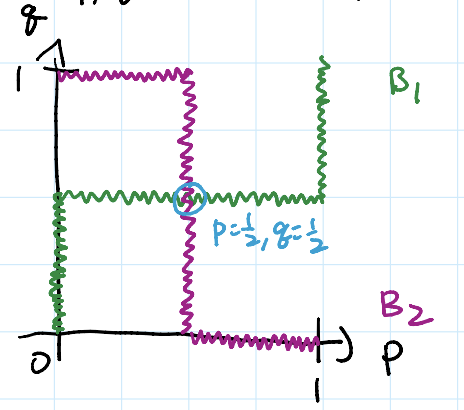
\includegraphics[]{matching_pennies_example.png}
	\end{figure}
\end{center}
\newpage
\begin{example}
	For the game of Bach or Stravinsky
	\begin{center}
		\begin{tabular}{|c|c|c|}
			\hline
			           & Bach & Stravinsky \\
			\hline
			Bach       & 2, 1 & 0, 0       \\
			\hline
			Stravinsky & 0, 0 & 1, 2       \\
			\hline
		\end{tabular}
	\end{center}
	Suppose $x^1 = (p, 1-p), x^2 = (q, 1-q)$. Then $u_1(B, x^2) = 2q$, $u_1(s, x^2) = 1-q$. So $u_1(x) = p(2q) + (1-p)(1-q) = p(-1+3q) + (1-q)$. Break into cases depending on $q = \frac{1}{3}$, and we get $$B_1(x^2) = \begin{dcases}
	\{(0, 1)\} & \text{ if } q < \frac{1}{3}\\
	\{(p, 1-p) : p \in [0, 1]\} & \text{ if } q = \frac{1}{3}\\
	\{(1, 0)\} & \text{ if } q > \frac{1}{3}\\
	\end{dcases}$$
	
	For player II, $u_2(x) = q(-2-3p) + 2 - 2p$.  Break into cases depending on $p = \frac{2}{3}$, and we get $$B_2(x^1) = \begin{dcases}
	\{(0, 1)\} & \text{ if } p < \frac{2}{3}\\
	\{(q, 1-q) : q \in [0, 1]\} & \text{ if } p = \frac{2}{3}\\
	\{(1, 0)\} & \text{ if } p > \frac{2}{3}\\
	\end{dcases}$$
	
	There are 3 intersections, so 3 NEs here. Two of them are pure strategies $((0, 1), (0, 1))$, and $((1, 0), (1, 0))$. And one is mixed strategy $((\frac{2}{3}, \frac{1}{3}), (\frac{1}{3}, \frac{2}{3}))$
\end{example}

\begin{center}
	\begin{figure}[h!]
		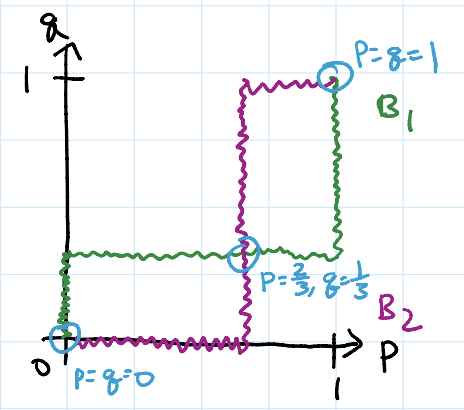
\includegraphics[]{Bach_or_Stravinsky_example.png}
	\end{figure}
\end{center}

\section{Support Characterization}

Recall that BRF maximizes a player's utility, $u_i(x) = \sum_{s \in S_i}x_s^iu_i(s, x^{-i})$. We multiply the probability that $s$ is selected ($x_s^i$), and the utility of playing $s$ as a pure strategy ($u_i(s, x^{-i})$). 

Suppose $\overline{x}^{-i}$ is fixed, which $x^i \in \Delta^i$ maximizes $u_i(x^i,\overline{x}^{-i})$? We can actually write it as a LP as P: \begin{align*}
\max &\sum_{s \in S_i}x_s^iu_i(s, x^{-i})\\
\text{ such that} &\sum_{s \in S_i}x_s^i= 1\\
&x^i \geq 0
\end{align*}

The variables are $x_s^i$ for each $s \in S_i$. What is the dual (D)? We have one dual variable $y$. \begin{align*}
\min & \;\;\;y\\
\text{ such that} & \;\;\;y \geq u_i(s, \overline{x}^{-i}) \text{ for all } s \in S_i
\end{align*}

Note that both $(P)$ and $(D)$ are feasible. $(P)$ is feasible because we can set $x^i$ to be any probability distribution. $(D)$ is feasible since we can set $y$ to be the max value of $u_i(s, \overline{x}^{-i})$. 

Therefore, $(P)$ and $(D)$ both have optimal solution, by the \textbf{Fundamental Theorem of LP}, and their optimal values are equal. 

Note that $(D)$ is easy to solve. $y = \max_{s \in S_i} u_i(s, \overline{x}^{-i})$, this is the maximum utility when pure strategies are played against $\overline{x}^{-i}$. So, $(P)$ also have optimal value $y$. So the maximum utility of all mixed strategies is equal to the max utility of pure strategies. 

Complementary slackness conditions are $x_s^i = 0$ or $y = u_i(s, \overline{x}^{-i})$ for all $s \in S_i$. Equivalently, $x_s^i > 0$ implies that $y = u_i(s, \overline{x}^{-i})$. Translation is that: only pure strategies with maximum utility could have positive positive probabilities in a best response. 

\begin{theorem}
	\textbf{\underline{Support Chracterization Theorem}}: Given $\overline{x}^{-i} \in \Delta^{-i}$, a mixed strategy $x^i \in B_i(\overline{x}^{-i})$ if and only if $x_s^i > 0$ implies $s\in S_i$ is a pure strategy of maximum utility against $\overline{x}^{-i}$.  
\end{theorem} 

\begin{definition}
	For a mixed strategy $x^i \in \Delta^i$, the \textbf{\underline{support}} is the set of strategies with positive probability in $x^i$. 
\end{definition}

\begin{theorem}
	\textbf{\underline{Support Chracterization Theorem}}: $x^i$ is in the BRF if and only if the support of $x^i$ are strategies with maximum utility. 
\end{theorem} 

\begin{example}
	For the game of Bach or Stravinsky
	\begin{center}
		\begin{tabular}{|c|c|c|}
			\hline
			           & Bach & Stravinsky \\
			\hline
			Bach       & 2, 1 & 0, 0       \\
			\hline
			Stravinsky & 0, 0 & 1, 2       \\
			\hline
		\end{tabular}
	\end{center}
	
	Suppose player II plays $x^2 = (q, 1-q)$, the utilities of player I using pure strategies are: $u_1(B, x^2) = 2q$, $u_1(S, x^2) = 1-q$. Depending on $q$, the strategies with maximum utility are different. \begin{enumerate}
	\item If $2q < 1-q$, then $q < \frac{1}{3}$, and $B$ is not in the support and gets probability 0. $BRF = \{(0, 1)\}$
	\item if $2q = 1-q$, then $q = \frac{1}{3}$, and both $B, S$ could be in the support. Any combination works, So $BRF = \{(p, 1-p) : p \in [0, 1]\}$
	\item If $2q > 1-q$, then $q > \frac{1}{3}$, and $S$ is not in the support. So $BRF = \{(1, 0)\}$
	\end{enumerate} 
	This matches the BRF we calculated previously. 
\end{example}

\begin{example}
	Consider the following game: 
	\begin{center}
		\begin{tabular}{|c|c|c|c|}
			\hline
			  & D    & E    & F    \\
			\hline
			A & 2, 2 & 3, 3 & 1, 1 \\
			\hline
			B & 3, 1 & 0, 4 & 2, 1 \\
			\hline
			C & 3, 4 & 5, 1 & 0, 7 \\
			\hline
		\end{tabular}
	\end{center}
	Suppose Player II plays $x^2 = (0, \frac{1}{3}, \frac{2}{3})$. What is $B_1(x^2)$? \begin{itemize}
	\item $u_1(A, x^2) = 0 + \frac{1}{3} \cdot 3 + \frac{2}{3} \cdot 1 = \frac{5}{3}$
	\item $u_1(B, x^2) = 0 + 0 + \frac{2}{3} \cdot 2 = \frac{4}{3}$
	\item $u_1(C, x^2) = 0 + \frac{1}{3} \cdot 5 + 0 = \frac{5}{3}$
	\end{itemize}
	So, playing $A$ and $C$ would yield max utility. So by the support characterization theorem, $x_B^1 = 0$. Any distribution over $x_A^1$ and $x_C^1$ would work. So $B_1(x^2) = \{(p, 0, 1-p) : p \in [0, 1]\}$. The maximum utility for player I is $p \cdot \frac{5}{3} + (1-p) \cdot \frac{5}{3} = \frac{5}{3}$, which is equal to the max utility for a pure strategy. 
	
	Any strategy in $B_1(x^2)$ maximizes the utility for player I. Which of these maximizes utility for player II? This will give us a NE. 
	
	Suppose $x^1 = (p, 0, 1-p)$. Calculate the utilities for player II is $u_2(D, x^1) = 4-2p$, $u_2(E, x^1) = 1+2p$, $u_2(F, x^1) = 7-6p$
	
	If $x^2 = (0, \frac{1}{3}, \frac{2}{3})$ is in the best response, then $E, F$ must have maximum utility. So $1+2p = 7-3p$, so $p = \frac{3}{4}$. 
	
	Utility for $E, F$ is $\frac{5}{2}$, utilities for $D$ is also $\frac{5}{2}$. So indeed, $E, F$ have maximum utility. So does $D$, but this is fine. 
	
	So $x^1 = (\frac{3}{4}, 0, \frac{1}{4})$, and $x^2 = (0, \frac{1}{3}, \frac{2}{3})$ are in the best responses for each other, and $(x^1, x^2)$ is a NE. 
\end{example}

Note: one ``algorithm'' for finding NE is by looking at possibile combinations of the supports for each player. In the example above, if we ask ``suppose support for player I is $\{A, C\}$, and support for player II is $\{E, F\}$'', then we can use the support characterization theorem to find a NE or prove the non exist for these supports. 

The problem is that, there are exponentially many support sets for each player, roughly $2^k$ if there are $k$ pure strategies. Not practical. 

Exercise: Show that in the game of rock paper scissors, both players playing $(\frac{1}{3}, \frac{1}{3},\frac{1}{3})$ is the only NE. 

\lecture{6}{October 20}{Martin Pei}{Haochen Wu}\\
This lecture's notes tend to be supplementary (add-on notes) of the course notes provided.

\section{Voting Game}

\begin{example}
	The example of \textbf{Voting Game}. 
		
	Downs paradox: voting has costs. The probability that one vote is decisive is very small. Costss outweigh benefits. The expectation is that people don't vote. However, in reality people do vote. 
		
	Let's model the vote participation. Suppose there are two candidates, $A, B$, and the number of supporters are $a, b$, respectively. Without loss of generality, assume $a \geq b$. Each person can choose to ``vote'' or ``abstain''. If they vote, then they incur a cost of $c$, where $0 < c < 1$. Regardless of voting or abstaining, each person gets a payoff of $2$ if their supporting candidate wins, 1 for a tie, and 0 for a loss. 
		
	For Pure NE, suppose $a = b = 1$, then the payoff table would be 
	\begin{center}
		\begin{tabular}{|c|c|c|}
			\hline
			  & A        & V          \\
			\hline
			A & 1, 1     & 0, $2-c$   \\
			\hline
			V & $2-c$, 0 & $1-c, 1-c$ \\
			\hline
		\end{tabular}
	\end{center}
		
	This is similar to prisoner's dilemma. If both players vote, they get lower utility than both players abstain. It's like the ``steal'' option here. 
		
	Suppose $a= b= 2$. There are 4 cases: \begin{itemize}
	\item Everyone votes. There is a tie, everyone has utility $1-c$, switching gives utility 0. So this is a NE. 
	\item Not everyone votes, but there is a tie. One who abstains can vote, the utility changes from 1 to $2-c$. This is not a NE. 
	\item One candidate wins by 1 vote. One who abstains for the losing candidate can vote. The utility changes from 0 to $1-c > 0$. This is not a NE. 
	\item One candidate wins by at least 2 votes. One who votes for the winning candidate can abstain, the utility changes from $2-c$ to $2$. This is not a NE.
	\end{itemize} 
	So, the only NE is everybody votes. Hence, in a close election, we expect more people to vote. 
	
	Exercise: when $a > b$, there is no NE. 
	
	For Mixed NE: there are a lot of, but hard to find. We discuss one possible scenario here. 
	
	Suppose $a > b$, among all $A$ supporters, $b$ of them will vote and $a-b$ of them will abstaion. Suppose every $B$ supporter will vote with the same probability $p$. So the best that $B$ can do is tie. It is easy to check that $p = 0$ or $1$ is not a NE. 
	
	Assume $p \in (0, 1)$. Consider a $B$ supporter. If they abstain, then $B$ cannot win. So the utility of ``abstain'' as a pure strategy is 0. If they vote, then $B$ ties only if all other supporters vote (gets utility $1-c$), otherwise $B$ loses (gets utility $-c$). 
	
	The expected utility of ``vote'' as a pure strategy is $p^{b-1}(1-c) + (1-p^{b-1})(-c)$, where $p^{b-1}$ is the probability that $b-1$ supporters vote, $(1-c)$ is the utility of a tie, $(1-p^{b-1})$ is the probability that not all of $b-1$ supporters vote, and $(-c)$ is the utility of a loss. This is equal to $p^{b-1} - c$. 
	
	When is it possible that this is in a NE? Since $p \in (0, 1)$, so both strategies have positive probabilities. To be in the best response, support characterization theorem implies that the two utilities are equal. So $0 = p^{b-1} - c$, or $p = c^{\frac{1}{b-1}}$. 
	
	Given this $p$, are $A$ supporters incentivized to change their mixed strategies? Currently, all of them are playing pure strategies. In order to switch, the utility of switching to the other pure strategy must be greater. \begin{itemize}
	\item Consider an $A$ supporter who abstained. Expected utility is $p^b \cdot 1 + (1-p^b)(2) = 2- p^b$. Expected utility of voting is $2-c$ ($A$ is guaranteed to win). So $2-c = 2-p^{b-1} \leq 2-p^b$ since $(0 < p < 1)$. 
		
	Switching to a pure strategy does not increase utility. So switching to any mixed strategy does not increase utility. No reason to switch. 
		
	\item Consider an $A$ supporter who voted. Expected utility is $\underbrace{p^b(1-c)}_\text{tie} + \underbrace{(1-p^b)(2-c)}_\text{win} = 2-p^b - c$. If they abstain, then \begin{itemize}
	\item $A$ loses if all $B$ supporters vote. 
	\item $A$ ties if $b-1$ supportes vote and 1 abstain. 
	\item $A$ wins.  
	\end{itemize}
	So the utility of abstaining is $p^b \cdot 0 + \underbrace{b}_\text{choices of who abstains} \cdot \underbrace{p^{b-1}}_{b-1 \text{ votes}} \cdot \underbrace{(1-p)}_\text{ 1 abstains} \cdot 1 + \underbrace{(1-p^b - b \cdot p^{b-1} (1-p))}_\text{remaining probability} \cdot 2 = 2-2p^b-bp^{b-1}(1-p)$
	
	We can check that $2-p^b - c \geq 2-2p^b-bp^{b-1}(1-p)$. So there is no reason to switch. 
	
	So, when $p = c^{\frac{1}{b-1}}$, this is a mixed NE. 
	
	What happens to voter participation as cost increases? If $c$ increases, then $p$ increases, so more voters will vote. 
	\end{itemize}
\end{example}
\section{Two-player zero-sum games}
\begin{definition}
	A strategic game is a \textbf{\underline{zero-sum}} game if for all strategy profiles $s \in S$, $\sum_{i \in N} u_i(s)  = 0$. 
\end{definition}

For example, matching pennies and rock paper scissors are all zero-sum games. 

For a two-player zero-sum game, let $S_1 = {1, ..., m}$, and $S_2 = \{1, ..., n\}$. Define such a game with a payoff matrix in $A \in \mathbb{R}^{m \times n}$, where $u_1(i, j) = A_{ij}$, and $u_2(i, j) = -A_{ij}$

\begin{example}
	For example, if we have the following matrix as the payoff for player I \begin{center}
	\begin{tabular}{|c|c|c|c|}
		\hline
		  & 1  & 2 & 3  \\
		\hline
		1 & 3  & 5 & -2 \\
		\hline
		2 & -5 & 7 & 1  \\
		\hline
	\end{tabular}
	\end{center} Then the payoff for player II would be \begin{center}
	\begin{tabular}{|c|c|c|c|}
		\hline
		  & 1  & 2  & 3  \\
		\hline
		1 & -3 & -5 & 2  \\
		\hline
		2 & 5  & -7 & -1 \\
		\hline
	\end{tabular}
	\end{center}
	The payoff are just negated. 
\end{example}
Note that for a mixed strategy profile $x = (x^1, x^2)$, $u_1(x^1, x^2) = -u_2(x^1, x^2)$. 

Min-Maxing argument for finding a NE: Given a strategy thay we play, the opposing player will maximize their utility, which minimizes our utility. Knowing how they would play, what can we do to maximize our own utility? 

From player I's perspective, suppose player I plays $x^1$. They expect player II to play from their best response. In the above example, $u_2(1, x^1) = -3x_1^1 + 5x_2^1, u_2(2, x^1) = -5x_1^1 -7x_2^1, u_2(3, x^1) = 2x_1^1-x_2^1$. So, player II's expected utility for playing a pure strategy $j$ is $$-(x^1)^TA_{\cdot j}$$ where $A_{\cdot j}$ is the $j$-th column of $A$. 

The utility of player II's best resonse is equal to the maximum of these values. In the example above, we look for $\max{-3x_1^1 + 5x_2^1, -5x_1^1 -7x_2^1, 2x_1^1-x_2^1}$. So, in general, we look for $$\max_{j \in \{1, ..., n\}} -(x^1)^TA_{\cdot j} = -\min_{j \in \{1, ..., n\}} (x^1)^TA_{\cdot j}$$

So the utility for player I is just $\min_{j \in \{1, ..., n\}} (x^1)^TA_{\cdot j}$. Player I wants to maximize this. So we want $\max \min_{j \in \{1, ..., n\}} (x^1)^TA_{\cdot j}$ where $\sum_{i=1}^m x_i^1 = 1$, $x^1 \geq 0$. 

This is not a LP. We need to linearize it. The final LP would be \begin{align*}
\max &\;\;u_1\\
\text{ such that} & \;\;u_1 \leq (x^1)^TA_{\cdot j} \;\;\;\;\forall j \in \{1, ..., n\}\\
&\;\;\sum_{i=1}^m x_i^1 = 1\\
&\;\;x^1 \geq 0
\end{align*}

From player II's perspective, suppose player II plays $x^2$. Then player I would play from their best response. 

With similar arguments, the utility of player I's best response is $$\max_{i \in \{1, ..., m\}} (x^2)^TA_{i\cdot}$$ where $A_{i\cdot }$ is the $i$-th row of $A$. 

Player II's utility would be $$-\max_{i \in \{1, ..., m\}} (x^2)^TA_{i\cdot}$$ Maximizing this would be equivalent to minimizing $\max_{i \in \{1, ..., m\}} (x^2)^TA_{i\cdot}$. So we get $\min \max_{i \in \{1, ..., m\}} (x^2)^TA_{i\cdot}$, where $\sum_{j=1}^{n}x_j^2 = 1$, $x^2 \geq 0$. With the same trick, the final LP would be 
\begin{align*}
	\min              & \;\;u_2                                                             \\
	\text{ such that} & \;\; (x^2)^TA_{i\cdot} \leq u_2 \;\;\;\;\forall i \in \{1, ..., m\} \\
	                  & \;\;\sum_{j=1}^n x_j^2 = 1                                          \\
	                  & \;\;x^2 \geq 0                                                      
\end{align*}

The main result is that, the LPs for player I and player II are duals of each other. 

Both LPs are feasible (take $x^1, x^2$ to be any probability distribution, $u_1, u_2$ has max/min values). So both have optimal solutions with the same objective value. (Note that objective value for player I's LP is the utility of player I, so the objective value for player II's LP is the negative of the utility of player II). So, the optimal solutions are best responses to each other. So they must form a NE. Solve for this using simplex. A modified version of simplex is probably in polynomial time, which is time-efficient.

\begin{theorem}
	Any two-player zero-sum game has a mixed Nash Equilibrium, and this can be efficiently computed. Assuming that there are finite pure strategies. 
\end{theorem}

For the example above, the optimal solution is \begin{itemize}
\item For player I, $x_1^1 = \frac{6}{11}$, $x_2^1 = \frac{5}{11}$, and $u_1 = -\frac{7}{11}$
\item For player II, $x_1^2 = \frac{3}{11}$, $x_2^2 = 0$, $x_3^2 = \frac{8}{11}$, and $u_2 = -\frac{7}{11}$
\item Note that $u_1$ is the utility for player I, and $-u_2$ is the utility of player II. 
\end{itemize}
Note that computing NE in general is difficult. Even in the 3-player-zero-sum game, or 2-player-general-sum game, no polynomial time algorithm is known. 

\section{Nash's Theorem}
\begin{theorem}
	\textbf{\underline{Nash's Theorem}}: Every Strategic game with finitely many players and pure strategies has a Nash Equilirbium. 
\end{theorem}
\begin{theorem}
	\textbf{\underline{Brouwer's Fixed Point Theorem}}: Let $x$ be a convex and compact set in a finite-dimensional Euclidean space, and let $f: X \rightarrow X$ be a continuous function. Then there exists $x_0 \in X$ such that $f(x_0) = x_0$. (``fixed point'')
\end{theorem}

\begin{example}
	Let $x \in [0, 1]$, consider any continuous function $f: [0, 1] \rightarrow [0, 1]$. The graph of $f$ will always intersect $f(x) = x$, producing a fixed point. This is a consequence of the intermediate value theorem, applying to $f(x) - x$. 
\end{example}

Terminology from the theorem: \begin{itemize}
\item We will think of an Euclidean space as $\mathbb{R}^n$ with the standard dot product, which defines how we measure distance and angle. 
\item A set is convex if for any two points in the set, the line segment joining them is also in the set. Precise definition is: $S$ is convex if for all $u, v \in S$, $\lambda u + (1-\lambda)v \in S$ for all $\lambda \in [0, 1]$. Note that the convex combination of any set of points in convex, i.e.  $S = \{\lambda_1v_1 + \cdots \lambda_nv_n : \lambda_1, ..., \lambda_n, \geq 0, \lambda_1 + \cdots \lambda_n = 1\}$. 
\item A set is compact if it is closed and bounded. Closed means that all ``boundary'' points are in the set. For example, $[0, 1]$ is closed, but $(0, 1)$ is not closed. Bounded means that there is a constant that bounds the distance between any two points. 
\end{itemize}

Note that this is a deep theorem from analysis. We will not prove it here, though there are many fascinating proofs of it. (Suggestion: look into the combinatorial proof using Sperner's Lemma). None of the proofs are constructive, we know that a fixed exists, but the proof does not tell us how to find one. 

Illustrations of Brouwer's Fixed Point Theorem: \begin{itemize}
\item print a world map and place it on your desk. This is a continuous mapping from the surface of the Earth to the part of the surface occupied by the map on your desk. The theorem tells us that there si a fixed point, i.e. some point on the map is directly on top of the point it represents on your desk. 
\item Take a cup of tea and stir it. Let it settle. Then some part of the liquid is in the same spot before the stir. 
\end{itemize}

Relate it back to strategic games. We want to use Brouwer's fixed point theorem when $X$ is the set of all mixed strategy profiles of a finite strategic game. We need to verify that $\Delta$ is convex and compact. 

We start with just one player $i$ and their set of mixed strategy $\Delta^i$. If the set of pure strategies is $\{1, ..., k\}$, then $$\Delta^i = \{(x_1^i, ..., x_k^i) : x_j^i \geq 0, x_1^i + \cdots x_k^i = 1\}$$

When $k = 2$, $\Delta^i = \{(p, 1-p) : p \in [0, 1]\}$. This is just a line segment in $\mathbb{R}^2$. When $k = 3$, $\Delta^i = \{(p, q, r) : p+q+r = 1, 0 \leq p, q, r \leq 1\}$. This is a triangle is $ \mathbb{R}^3$
\begin{center}
	\begin{figure}[h!]
		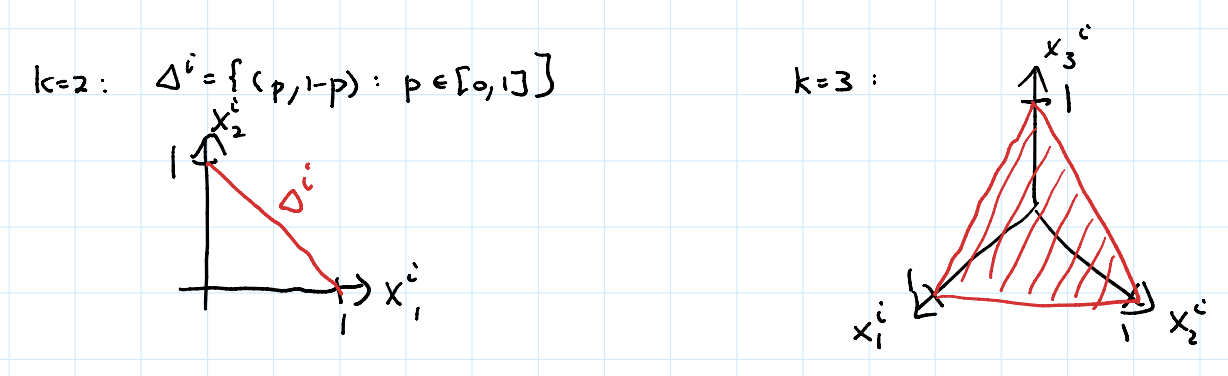
\includegraphics[width=\linewidth]{Delta_is_convex_and_compact.png}
	\end{figure}
\end{center}

We can see that (without proof) $\Delta^i$ is compact. It is closed, and any 2 points have distance at most 1. $\Delta^i$ is convex. It is the convex combination of the standard basis vectors $e_1, ..., e_k$ (an element of $\Delta^i$ has the form $x_1^ie_1 + \cdots + x_k^ie_k$, where $x_1^i + \cdots x_k^i = 1$, $x_j^i \geq 0$). These $e_1, ..., e_k$ are the pure strategies of player $i$. 

The set of all strategy profiles is $\Delta = \Delta^1 \times \cdots \times \Delta^n$. We can ``pretend'' that this is a set in $\mathbb{R}^{|S_1| + \cdots + |S_n|}$. It is still compact (a result from analysis is that the cartesian product of compact sets is compact). It is also convex. So we can use $\Delta$ as the set in Brouwer's Fixed Point Theorem. Then, we need to find a continuous function $f: \Delta \rightarrow \Delta $ that relates fixed points to mixed Nash equilibira. 

The main idea is that, given a strategy profile $x = (x^1, ..., x^n)$, a player $i$ will look at possibly switching to a pure strategy to gain utility against $x^{-i}$. If pure strategy $s$ improves utility, then player $i$ wants to shift the probability distribution so that $s$ receives higher probability. 

The function will take $x$ and map it to another strategy profile where each player improves their utility. 

For the example in Rock Paper Scissors. 
	
Suppose both play rock as a pure strategy, they can increase utility moving toward paper. 
\begin{center}
	\begin{figure}[h!]
		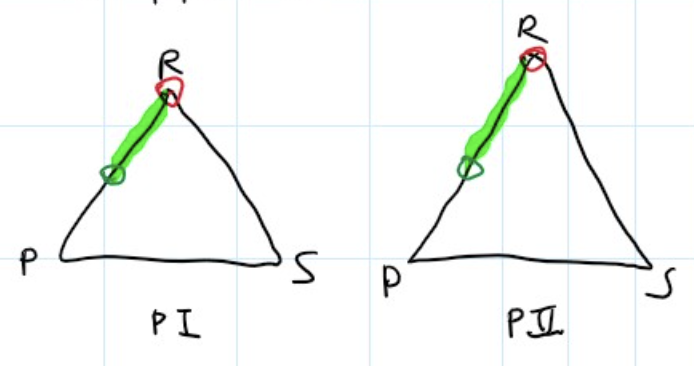
\includegraphics[width=250pt]{Rock_Paper_Scissors_1.png}
	\end{figure}
\end{center}
\newpage
Suppose player I plays rock, and player II plays paper. Player II cannot improve utility. Player I can improve utility by 1 if they move to paper, improve utility by 2 if they move to scissors. Player I will move more towards scissors than paper. 
\begin{center}
	\begin{figure}[h!]
		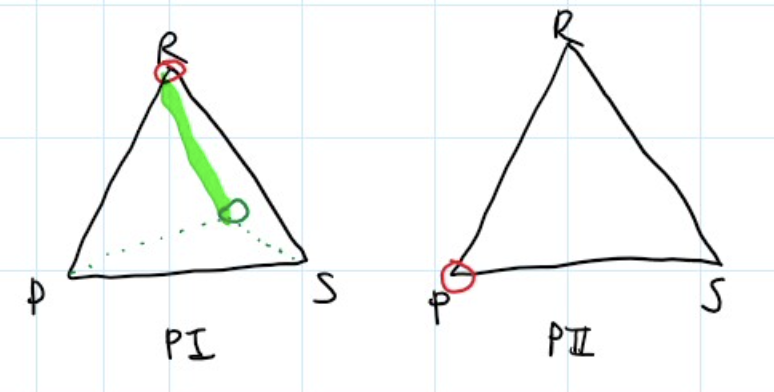
\includegraphics[width=250pt]{Rock_Paper_Scissors_2.png}
	\end{figure}
\end{center}

What is the meaning of a fixed point? It means that no player can improve their utility. So, it has to be a NE. 

Defining the function: 

First, define $\Phi$ which records the improvement of a player in switching to a pure strategy. Given a strategy profile $x \in \Delta$, and a pure strategy $s \in S_i$, define $\Phi_s^i(x) = \max\{0, u_i(s, x^{-i}) - u_i(x)\}$. 

If playing $s$ increases utility for player $i$, then $\Phi_s^i(x)$ represents this increase. Otherwise, $\Phi_s^i(x)$ is 0. 

For player $i$ and strategies $s$ where $\Phi_s^i(x) > 0$, we want to increase probability on $s$. 

We want to replace $x_s^i$ by $x_s^i + \Phi_s^i(x)$, but the sum of the probabilities is greater than 1. We can normalize this by dividing by $\sum_{s' \in S_i}(x_{s'}^i + \Phi_{s'}^i(x)) = 1 + \sum_{s' \in S_i}\Phi_{s'}^i(x)$. 

We define $f: \Delta \rightarrow \Delta$ by $f(x) = \bar{x}$ where for each player $i$ and strategy $s \in S_i$, $\bar{x}_s^i = \frac{x_s^i + \Phi_s^i(x)}{1 - \sum_{s' \in S_i}\Phi_s^i(x)}$. 

We may verify that $f(x) \in \Delta$. 

\begin{example}
	In rock paper scissors where player I plays rock and player II plays paper. The strategy profile is $x = ((1, 0 , 0), (0 , 1, 0))$. 
		
	For player II, $\Phi_s^2(x) = 0$ for each $s \in \{R, P, S\}$. For player I, $\Phi_R^1(x) = 0$, $\Phi_P^1(x) = 1$, $\Phi_S^1(x) = 2$. So the new strategy for player I is $\bar{x}_R^1 = \frac{1+0}{1+3} = \frac{1}{4}$, $\bar{x}_P^1 = \frac{0+1}{1+3} = \frac{1}{4}$, $\bar{x}_R^1 = \frac{0+2}{1+3} = \frac{1}{2}$. So, $f(x) = ((\frac{1}{4}, \frac{1}{4}, \frac{1}{2}), (0, 1, 0))$. 
\end{example}

Completing the proof of Nash's Theorem: 

Given $x \in \Delta$, consider $\Phi$ and $f: \Delta \rightarrow \Delta$ as defined above. We see that $f$ is continuous since $\Phi$ is continuous. By Brouwer's fixed point theorem, there exists $\hat{x} \in \Delta$ such that $f(\hat{x}) = \hat{x}$. We prove that $\hat{x}$ is a NE by showing $\hat{x}^i \in B_i(\hat{x}^{-i})$. 

For player $i$, let $s \in S_i$ be a pure strategy such that $\hat{x}^i > 0$ and $u_i(s, \hat{x}^{-i}) \leq u_i(\hat{x})$ (exercise: shows that $s$ exists). Then $\Phi_s^i(\hat{x}) = 0$. Since $\hat{x}$ is a fixed point, $\hat{x}_s^i = (f(\hat{x}))_s^i = \hat{x}_s^i / (1 + \sum_{s' \in S_i} \Phi_{s'}^i(\hat{x}))$. Since $\hat{x}_s^i > 0$, the denominator must be 1. So $\sum_{s' \in S_i} \Phi_{s'}^i(\hat{x}) = 0$. But $\Phi$ is non-negative. So $\Phi_{s'}^i(\hat{x}) = 0$ for all $s' \in S_i$. This means that $u_i(s', \hat{x}^{-i}) \leq u_i(\hat{x})$ for all $s' \in S_i$. So playing $\hat{x}^i$ gives the highest utility against $\hat{x}^{-i}$, so $\hat{x}^i \in B_i(\hat{x}^{-i})$. 

Since this holds for all players, $\hat{x}$ is a Nash equilibrium. 

Note that this proves that a NE always exists. But the proof does not show us how to find such a NE, as it depends on Brouwer's fixed point theorem. 



\lecture{7}{October 27}{Martin Pei}{Haochen Wu}\\
This lecture's notes tend to be supplementary (add-on notes) of the course notes provided.
\section{Cooperative Games}
There are games where groups of players can work together to obtain higher utility. 

\begin{definition}
	A cooperative game is given by a set of players $N$ and a characteristic function $v: 2^N \rightarrow \mathbb{R}$ that assigns a value $v(S)$ to each coalition $S \subseteq N$ of players. We use $(N, v)$ to represent this game. The set $N$ is the grand coalition. 
\end{definition}

\begin{example}
	$A, B, C$ want to buy ice cream. There are 3 sizes of ice cream: 1L, 1.5L, 2L with costs \$7, \$9, \$11. $A$ has \$3, $B$ has \$4, $C$ has \$5. On their own, they cannot buy any. But if they pool money together, they can get some icecream.
		
	In this case $N = \{A, B, C\}$, and $v$ is defined by: \begin{center}
	\begin{tabular}{|c|c|c|c|c|c|}
		\hline
		$S$    & $\emptyset, \{A\}, \{B\}, \{C\}$ & $\{A, B\}$ & $\{A, C\}$ & $\{B, C\}$ & $\{A, B, C\}$ \\
		\hline
		$v(S)$ & 0                                & 1          & 1          & 1.5        & 2             \\
		\hline
	\end{tabular}
	\end{center}
\end{example}
In general, $v(\emptyset) = 0$, $v(S) \geq 0$ for all $S \subseteq N$. 

\begin{example}
	A country has a 101-member parliament. There are 4 parties, $A, B, C, D$ with 40, 22, 30, 9 members, respectively. They need to decide how to spend \$1 billion winfall. They need to form a majority to spend it. 
		
	In this case, $N = \{A, B, C, D\}$. $$V(S) = \begin{dcases}
	10^9 & \text{ if parties in } S \text{ has } \geq 51 \text{ members}\\
	0 & \text{ otherwise}
	\end{dcases}$$
\end{example}

\begin{example}
	In a matching game, we are given a grpah $G = (V, E)$ and edge weights $w: E \rightarrow \mathbb{R}$. They players are the vertices, $V = N$. The weight of an edge represents the benefits if the two vertex players work together. 
		
	For any subset $S \subseteq N$, the value is the maximum weight of a matching using vertices in $S$. 
\end{example}
\begin{center}
	\begin{figure}[h!]
		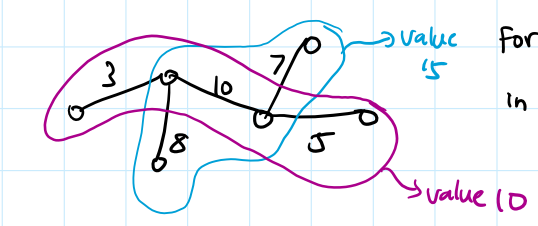
\includegraphics[]{matching_game.png}
	\end{figure}
\end{center}

\begin{itemize}
	\item Outcome of strategic games are strategy profiles (pure or mixed), .i.e which strategy is played by each player? 
	\item Outcome of cooperative games: \begin{itemize}
	\item Divide the players into groups, we call them coalitions. \textbf{``coalition structure''}
	      		
	      Each coalition will generate their assigned value
	\item Distribute the value that each coalition generates among its members \textbf{``payoff vector''}
\end{itemize}
\end{itemize}
\begin{definition}
	Given a cooperative game $(N, v)$, a \textbf{\underline{coalition structure}} is a partition $\pi$ of $N$, i.e. $\pi = (C^1, ..., C^k)$ where each $c^i \subseteq N$, $C^i \cap C^j = \emptyset$ whenever $i \neq j$, and $C^1 \cup \cdots \cup C^k = N$
		
	A \textbf{\underline{payoff vector}} is a vector $x \in \mathbb{R}^N$ such that $x \geq \vec{0}$ and $\sum_{i \in C^j} x_i \leq v(C^j)$ for all $j = 1, ..., k$. 
		
	Notation: For any $T \subseteq N, x(T) = \sum_{i \in T}^{x_i}$, so the inequality above becomes $x(C^j) \leq v(C^j)$. 
		
	An outcome consists of $(\pi, x)$. Such an outcome is \textbf{\underline{efficient}} if $x(C^j) = v(C^j)$ for all $j$
\end{definition}

\begin{example}
	An outcome of the ice cream game is $(\pi, x)$, where $\pi = (\{A, B\}, \{C\})$, and $x_A = 0.5, x_B = 0.5, x_C = 0$. This outcome is efficient since $v(\{A, B\}) = 1 = x_A + x_B$, $v(\{C\}) = x_C = 0$. 
\end{example}

There are some classes of games: 
\begin{definition}
	\textbf{\underline{Monotone games}}: For any $S \subseteq T$, we have $v(S) \leq V(T)$. This literally means that ``more people produce more value''
\end{definition}

\begin{definition}
	\textbf{\underline{Superadditive games}}: For any disjoint $S, T$, we have $v(S) + v(T) \leq v(S \cup T)$. This means that ``forming coalitions is always better''
		
	Note that superadditive $\Rightarrow$ monotone, however, the converse is not true. We usually only consider the grand coalition $\pi = (N)$. 
\end{definition}

\begin{definition}
	\textbf{\underline{Convex games}}: For any $S, T$, we have $v(S) + v(T) \leq v(S \cup T) + v(S \cap T)$. This is also known as ``supermodularity inequality''
		
	Note that convexity $\Rightarrow$ superadditivity, however, the converse is not true. 
\end{definition}

\begin{theorem}
	A game $(N, v)$ is convex if and only if for every $S, T$ where $S \subseteq T \subseteq N$, and for any player $i \in N \setminus T$, we have $v(T \cup \{i\}) - v(T) \geq v(S \cup \{i\}) - v(S)$
		
	This means that ``a player is more useful in larger coalitions''
\end{theorem}

\section{Shapley Values}
There are two desirable properties of an outcome in cooperative games: \begin{enumerate}
\item Faireness. The payoff vector should reflect the contribution of the players to their coalitions
\item Stability. We want to incentivize the players to stay in their assigned coalition in the coalition structure
\end{enumerate}

\textbf{\underline{Shapley values}} deals with the fairness of the payoff vector. Assume players form the grand coalition. (if not, we can look at individual coalitions separately)

Q: How to quantify a players contribution? There are several ideas: \begin{enumerate}
\item We can compare the value of coalition before and after a player joins it. 
	
For example, in the ice cream game. The contribution of $A$ is $v(\{A, B, C\}) - v(\{B, C\}) = 0.5$. The contribution of $B$ is 1, and the contribution of $C$ is 1. 
	
But a payoff vector cannot take these values, since the sum may exceed the value of the coalition. $x(N) > v(N)$. 
	
\item Fix a sequence of players, and see their contribution sequentially. 
	
For example, in the ice cream game, use the sequence $A, B, C$. The contribution of $A$ is $v(\{A\}) = 0$. $v(\{A, B\}) = 1$, so $B$ contributes 1. $v(\{A, B, C\}) = 2$, so $C$ contributes 1. This is efficient. $x(N) = v(N)$. 
	
But, different orderings produce different payoffs
	
\item Shapley's idea: look at all possible orderings of the players, average a player's contributions.
	
We introduce new notation here: A permutation of $N$ has the form $\sigma = (\sigma_1, ..., \sigma_n)$ where each $\sigma_i$ is a distinct element of $N$. The leemnt $\sigma_i$ is at the $i$-th position of $\sigma$. The set of all permutations of $N$ is denoted as $S_N$. 
\end{enumerate}

\begin{definition}
	Given a permutatioon $\sigma \in S_N$, the \textbf{\underline{marginal contribution}} of player $\sigma_i$ is $$\Delta_\sigma(\sigma_i) = v(\{\sigma_1, ..., \sigma_i\}) - v(\{\sigma_1, ..., \sigma_{i-1}\})$$
		
	The \textbf{\underline{Shapley value}} of player $i$ is $$\varphi_i = \frac{1}{n!}\sum_{\sigma \in S_N} \Delta_\sigma(i)$$
\end{definition}

\begin{example}
	In the ice cream game. $N = \{A, B, C\}$, and there are 6 permutations. $$\sigma^1 = (A, B, C), \sigma^2 = (A, C, B), \sigma^3 = (B, A, C), \sigma^4 = (B, C, A), \sigma^5 = (C, A, B), \sigma^6 = (C, B, A)$$
		
	We calculate the marginal contribution of $A$ in each of the permutations: \begin{itemize}
	\item $\Delta_{\sigma^1}(A) = v(\{A\}) - v(\emptyset) = 0$
	\item $\Delta_{\sigma^2}(A) = v(\{A\}) - v(\emptyset) = 0$
	\item $\Delta_{\sigma^3}(A) = v(\{B, A\}) - v(\{B\}) = 1$
	\item $\Delta_{\sigma^4}(A) = v(\{B, C, A\}) - v(\{B, C\}) = 0.5$
	\item $\Delta_{\sigma^5}(A) = v(\{C, A\}) - v(\{C\}) = 1$
	\item $\Delta_{\sigma^6}(A) = v(\{C, B, A\}) - v(\{C, B\}) = 0.5$
	\end{itemize}
	So the Shapley value of $A$ is $$\varphi_A = \frac{1}{6}(0+0+1+0.5+1+0.5) = \frac{1}{2}$$
	
	The Shapley value of $B$ and $C$ are $\varphi_B = \varphi_C = \frac{3}{4}$
\end{example}

There are 4 good properties of Shapley value: \begin{enumerate}
\item Efficiency. 
\item Symmetric.
\item Dummy player.
\item Additivity. 
\end{enumerate}
\begin{theorem}
	$\sum_{i \in N} \varphi_i= v(N)$. 
\end{theorem}
\begin{proof}
	For any $\sigma \in S_N$, the sum of all marginal contribution is\begin{align*}
	\sum_{i \in N} \Delta_\sigma(i) &= \sum_{i=1}^{n} \Delta_\sigma (\sigma_i)\\
	&=[v(\{\sigma_1\}) - v(\emptyset)] + [v(\{\sigma_1, \sigma_2\}) - v(\{\sigma_1\})] + \cdots + [v(\{\sigma_1, ..., \sigma_n\}) - v(\{\sigma_1, ..., \sigma_{n-1}\})]\\
	&=v(\{\sigma_1, ..., \sigma_n\}) - v(\emptyset)\\
	&=v(N)
	\end{align*}
	So the sum of Shapley values is $$\sum_{i \in N} \varphi_i = \sum_{i \in N} \frac{1}{n!} \sum_{\sigma \in S_N} \Delta_\sigma (i) = \frac{1}{n!} \sum_{i \in N} \sum_{\sigma \in S_N} \Delta_\sigma (i) = \frac{1}{n!} \sum_{\sigma \in S_N} v(N) = \frac{1}{n!} (n!) v(N) = v(N)$$
\end{proof}

\begin{definition}
	Two players $i, j$ are \textbf{\underline{symmetric}} if $v(C \cup \{i\}) = v(C \cup \{j\})$ for all $C \subseteq N \setminus \{i, j\}$. This means they contribute to coalitions equally. 
\end{definition}

\begin{theorem}
	If $i, j$ are symmetric players, then $\varphi_i = \varphi_j$. 
\end{theorem}
\begin{proof}
	The idea is to swap $i, j$ in the permutation, and compute the Shapley values accordingly. 
		
	Let's define $f: S_N \rightarrow S_N$ where $f(\sigma)$ is obtained from $\sigma$ by swapping $i$ and $j$. This is a bijection since $f^{-1} = f$. 
		
	We claim that $\Delta_\sigma (i) = \Delta_{f(\sigma)}(j)$. There are two cases: \begin{itemize}
	\item Suppose $i$ preceeds $j$ in $\sigma$. Let $C$ be all elements preceeding $i$. In $f(\sigma)$, $C$ is also the elements that preceed $j$. So $\Delta_\sigma (i) = v(C \cup \{i\}) - v(C)$ and $\Delta_{f(\sigma)} (j) = v(C \cup \{j\}) - v(C)$. 
			
	Since $C \subseteq N \setminus \{i, j\}$, and $i, j$ are symmetric, $v(C \cup \{i\}) = v(C \cup \{j\})$. So $\Delta_\sigma (i) = \Delta_{f(\sigma)} (j)$. 
			
	\item Suppose $j$ preceeds $i$. Let $C$ be all elements preceeding $i$ except $j$. In $f(\sigma)$, $C$ is also the elements that preceeds $j$ except $i$. 
			
	So, $\Delta_\sigma(i) = v(C \cup \{j\} \cup \{i\}) - v(C \cup \{j\})$ and $\Delta_{f(\sigma)}(j) = v(C \cup \{i\} \cup \{j\}) - v(C \cup \{i\})$. 
			
	Since $C \subseteq N \setminus \{i, j\}$, and $i, j$ are symmetric, $v(C \cup \{j\}) = v(C \cup \{i\})$, so $\Delta_\sigma (i) = \Delta_{f(\sigma)} (j)$. 
	\end{itemize}
	
	Therefore, $$\varphi_i = \frac{1}{n!} \sum_{\sigma \in S_N} \Delta_\sigma(i) = \frac{1}{n!} \sum_{\sigma \in S_N} \Delta_{f(\sigma)} (j) = \frac{1}{n!} \sum_{\sigma \in S_N} \Delta_\sigma (j) = \varphi_j$$
\end{proof}

\begin{example}
	In an unanimy game. Suppose $|N| = n$, and $v(S) = \begin{dcases}
	1 & S = N\\
	0 & \text{otherwise}
	\end{dcases}$. Any pair of players is symmetric, so $\varphi_i = \varphi_j$ for any $i, j$. Since $\varphi$ is efficient, the sum is $v(N) = 1$. So $\varphi_i = \frac{1}{n}$ for each $i \in N$
\end{example}

\begin{definition}
	$i$ is a \textbf{\underline{dummy player}} if $v(S \cup \{i\}) = v(S)$ for all $S \subseteq N \setminus \{i\}$. The player does not contribute to any coalition. 
\end{definition}
\begin{example}
	In a 101-seat parliament, $A, B, C, D$ with 40, 22, 30, 9 seats. Party $D$ is a dummy player. No combination of $A, B, C$ exists where it is not a majority but adding $D$ is gives a majority. 
\end{example}

\begin{theorem}
	If $i$ is a dummp player, then $\varphi_i = 0$. 
\end{theorem}

\begin{proof}
	For any $\sigma \in S_N$, say $i$ is at the $j$-th position ($\sigma_j = i$). The marginal contribution of $i$ is $$\Delta_\sigma (i) = v(\{\sigma_1, ..., \sigma_{j-1}, \sigma_i\}) - v(\{\sigma_1, ..., \sigma_{j-1}\}) = 0$$ by definition of a dummy player. So $$\varphi_i = \frac{1}{n!} \sum_{\sigma \in S_N} \Delta_\sigma(i)  = 0$$
\end{proof}

Note that the converse of this theorem is not true. If a game is monotone, then the converse is true. 

\begin{definition}
	\textbf{\underline{Additivity}}: Suppose there are multiple games with the same set of players. We add the values together to get a new game. Then, the Shapley values are also added together. 
\end{definition}

\begin{theorem}
	Let $(N, v^1), (N, v^2)$ be two cooperative games. Define $v^3(S) = v^1(S) + v^2(S)$ for all $S \subseteq N$. Let $\varphi_i^j$ be the Shapley values of player $i$ in $(N, v^j), j = 1, 2, 3$. Then $\varphi_i^3 = \varphi_i^1 + \varphi_i^2$. 
\end{theorem}

Summary: The Shapley values satisfy 4 good properties which are efficiency, symmetric, dummy player, and additivity. 

The deeper result is that: the Shapley value function is the only one that satisfies all of these 4 properties. In other words, if $f$ is a function that maps $(N, v)$ to a real vector $\mathbb{R}^N$, and all 4 properties hold, then $f$ gives the Shapley values. 


\lecture{8}{November 3}{Martin Pei}{Haochen Wu}\\
This lecture's notes tend to be supplementary (add-on notes) of the course notes provided.
\section{The Core}
Stability: Given an outcome, what could be a reason that players want to deviated from it? A group of players could generate more value that what they are receiving, i.e. $x(C) < v(C)$.

\begin{definition}
	The \textbf{\underline{core}} of a cooperative game $(N, v)$ consists of all outcomes $(\pi, x)$ such that $x(C) \geq v(C)$ for all $C \subseteq N$
\end{definition}

\begin{example}
	In the example of ice cream game, consider $(\pi, x)$ with $\pi = (\{A, B\}, \{C\})$ and $x_A = x_B = 0.5, x_C = 0$. If $C$ joins with $\{A, B\}$, then they produce 2, while currently their combined payoffs is 1. It is better if they form $\{A, B, C\}$, so such $(\pi, x)$ is not in the core.
		
	Same reasoning for $\pi = (N)$. If $(\pi, x)$ is in the core, then if $x_A = 2, x_B = x_C = 0$, then $\{B, C\}$ can get more value. If $x_A = 0, x_B = x_C = 1$, then $(\pi, x)$ is in the core. This satisfies these inequalities: $$x_A + x_B + x_C \geq 2, x_A + x_B \geq 1, x_A + x_C \geq 1, x_B + x_C \geq 1.5, x_A \geq 0, x_B \geq 0, x_C \geq 0$$
\end{example}

Properties of the outcomes in the core: \begin{enumerate}
\item They are efficient with the coalition structure
\item The coalition structure generates the maximum amount of total value among all outcomes. Also known as ``social welfare''
\end{enumerate}

We introduce a notation $$v(\pi) = \sum_{C \in \pi} v(C)$$

\begin{theorem}
	If $(\pi, x)$ is in the core, then $x(C) = v(C)$ for each $C \in \pi$
\end{theorem}
\begin{proof}
	Let $C \in \pi$. By the definition of the core, $x(C) \geq v(C)$. Since $(\pi, x)$ is a valid outcome, $x(C) \leq v(C)$. So $x(C) = v(C)$ for all $C \in \pi$. 
\end{proof}

\begin{theorem}
	If $(\pi, x)$ is in the core, then $v(\pi) \geq v(\pi')$ for all partitions $\pi'$ of $N$. 
\end{theorem}

\begin{proof}
	\begin{align*}
		v(\pi) & = \sum_{C \in \pi}v(C)                                                      \\
		       & =\sum_{C \in \pi}x(C) \text{ by Theorem 8.130}                              \\
		       & =\sum_{i \in N}x_i \text{ Since } \pi \text{ is ia partition of }N          \\
		       & =\sum_{C' \in \pi'}x(C) \text{ Since } \pi' \text{ is a partition of }N     \\
		       & \geq \sum_{C' \in \pi'} v(C') \text{ Since }(\pi, x) \text{ is in the core} \\
		       & =v(\pi')                                                                    
	\end{align*}
\end{proof}

Note that this proposition only says that coalition structures that maximize total value are eligible to be in the core. It does not mean that there exists an outcome in the core with this structure. 

There exists some games with empty cores. 

\begin{example}
	3-player majority game. Let $N = \{1, 2, 3\}$, $v(S) = \begin{dcases}
	1 & |S| \geq2 \\ 0 & \text{otherwise}
	\end{dcases}$. We claim that no outcome is in the core. Suppose $(\pi, x)$ is in the core. Then, $x_1 + x_2 + x_3 \geq 1, x_1, x_2, x_3 \geq 0$. So $x_i \geq \frac{1}{3}$ for some $i$. The value of any coalition is at most 1, so $x_1+x_2 + x_3 \leq 1$. This means that $x(N \setminus \{i\}) \leq \frac{2}{3}$. However, $v(N \setminus \{i\}) = 1 > x(N \setminus \{i\})$. This contradicts the assumption that $(\pi, x)$ is in the core. Hence, core is empty. 
\end{example}

\section{Cores of Superadditive Games}
Our goal is to determine when a superadditive game has a non-empty core. 

We can narrow down the search to that we only need to consider outcomes that form the grand coalition. 

\begin{theorem}
	Let $(N, v)$ be a superadditive game. If $(\pi, x)$ is in the core, then $((N), x)$ is in the core.
\end{theorem}

\begin{proof}
	We need to prove that the core conditions hold, and $((N), x)$ is a valid outcome. 
		
	Since $(\pi, x)$ is in the core, $x(C) \geq v(C)$ for all $C \subseteq N$. This still holds for $((N), x)$. 
		
	To show that $((N), x)$ is a valid outcome, we need to show that $x(N) \leq v(N)$ \begin{align*}
	x(N) &= \sum_{C \in \pi} x(C) \text{ since } \pi \text{ is a partition of }N\\
	&\leq \sum_{C \in \pi} v(C) \text{ since }(\pi, x) \text{ is a valid outcome}\\
	&\leq v(N) \text{ superadditivity}
	\end{align*}
\end{proof}

\begin{example}
	In the unanimity game, we have $v(S) = \begin{dcases}
	1 & S = N \\ 0 &\text{otherwise}
	\end{dcases}$. To determine if the core is empty, we only need to consider $((N), x)$. $x$ satisfies $\sum_{i \in N} x_i = 1$ by theorem 8.130, and $\sum_{i \in S}x_i \geq 0$ for all $S \subseteq N$. For example, we can let $x_i = \frac{1}{n}$ for all $i$. Or, we can have $x_1 = 1$, $x_i = 0$ for $i \neq 1$. 
\end{example}

Characterizing Superadditive games with non-empty cores

Given an outcome $((N), x)$, what must $x$ satisfy to be in the core? We claim that $x$ must be in the set $$\mathcal{C} = \{x \in \mathbb{R}^N : \underbrace{x(N) = v(N)}_\text{ by theorem 8.130}, \underbrace{x(C) \geq v(C) \; \text{ for all } C \subseteq N}_\text{ by definition of the core}\}$$

\begin{example}
	in the ice cream game, $\mathcal{C} = \{x \in \mathbb{R}^N : x_A + x_B + x_C = 2, x_A + x_B \geq 1, x_A + x_C \geq 1, x_B + x_C \geq 1.5, x_A \geq 0, x_B \geq 0, x_C \geq 0, x_A + x_B + x_C \geq 2\}$
\end{example}

Now, $\mathcal{C}$ is the intersection of halfspaces, so it is a polyhedron. 

Mini-result: $(N, v)$ has a non-empty core if and only if $\mathcal{C}$ is non-empty. 

We can solve the problem if ``is $\mathcal{C}$ non-empty'' using a linear program: 

Let $(P)$ be the following LP: \begin{align*}
\min &\;\;\;x(N)\\
\text{ such that} &\;\;\;x(C) \geq v(C) \text{ for all } C \subseteq N
\end{align*}

Taking the dual (D): \begin{align*}
\max &\;\;\;\sum_{C \subseteq N} y_Cv(C)\\
\text{ such that} &\;\;\;\sum_{C \subseteq N, i \in C} y_C = 1 \text{ for all } i \in N\\
& y \geq \vec{0}
\end{align*}

\begin{example}
	For the ice cream example, $(P)$ is \begin{align*}
	\min & \;\;\; x_A + x_B + x_C\\
	\text{ such that}&\;\;\;x_A \geq 0\\
	&\;\;\;x_B \geq 0\\
	&\;\;\;x_C \geq 0\\
	&\;\;\;x_A + x_B \geq 1\\
	&\;\;\;x_A + x_C \geq 1\\
	&\;\;\;x_B + x_C \geq 1.5\\
	&\;\;\;x_A + x_B + x_C \geq 2
	\end{align*}
	and $(D)$ is \begin{align*}
	\max & \;\;\; y_{AB} + y_{AC} + 1.5y_{BC} +2y_{ABC}\\
	\text{ such that}&\;\;\;y_A + y_{AB} + y_{AC} + y_{ABC} = 1\\
	&\;\;\;y_B + y_{AB} + y_{BC} + y_{ABC} = 1\\
	&\;\;\;y_C + y_{AC} + y_{BC} + y_{ABC} = 1\\
	&\;\;\;y\geq \vec{0}
	\end{align*}
\end{example}

Rationale: $(P)$ is feasible, since we can take arbitrarily large $x$, and $x(N) \geq v(N)$ is a constraint. So $(P)$ is bounded. By Fundamental Theorem of Linear Programming, $(P)$ has an optimal solution. If optimal value is $v(N)$, then we have optimal solution $x$ with $x(N) = v(N)$ and $x(C) \geq v(C)$ for all $C \subseteq N$, so $x \in \mathcal{C}$. 

Mini-result: $(N, v)$ has a non-empty core if and only if $(P)$ has optimal value $v(N)$. 

Also, notice that, $(P)$ has optimal value $v(N)$ $\Leftrightarrow$ $(D)$ has optimal value $v(N)$ $\Leftrightarrow$ $\sum_{C \subseteq N} y_Cv(C) \leq v(N)$ for all possible $y$. 

Subtle point: Is it possible that $\sum_{C \subseteq N} y_Cv(C) < v(N)$ for all $y$? 

What is the meaning of the dual? \begin{enumerate}
\item Feasible solution: $\sum_{C \subseteq N, i \in C} y_C = 1$. For example, $y_{AB} = y_C = 1$, which correspond to $(\{A, B\}, \{C\})$; or $y_{ABC} = 1$, which correspond to $(\{A, B, C\})$; or $y_{AB} = y_{BC} = y_{AC} = \frac{1}{2}$, which correspond to ``fractional partition'', a world for $\{A, B\}$ $\frac{1}{2}$ of the time, $\{A, C\}$ $\frac{1}{2}$ of the time. Total 1 for $A$. 
	
A feasible solution $y$ is a generalized coalition structure, $y_C$ represents the fraction of time each member will contribute to $C$, with a total time of $1$ from each player. Any such feasible $y$ is called a \textbf{\underline{balancing weight}}.
	
\item Objective: $\sum_{C \subseteq N} y_Cv(C) \leq v(N)$. For example, $y_{AB}v(\{A, B\}) + y_Cv(\{C\}) \leq 2$, $$\underbrace{v(\{A, B\}) + v(\{C\})}_{\text{value of the coalition structure} (\{A, B\}, \{C\})} \underbrace{\leq}_\leq \underbrace{2}_{\text{value of the grand coaltion} (N)}$$
	
By Theorem 8.132, this is maximize social welfare. 
	
Then, $\sum_{C \subseteq N} y_Cv(C)$ is the total value of the fractional partition represented by $y$. The inequality $\sum_{C \subseteq N} y_Cv(C) \leq v(N)$ means the value of the grand coalition is maximum over the values of any fractional partition. This generalizes Theorem 8.132. 
\end{enumerate}

\begin{definition}
	A feasible solution $y$ is a generalized coalition structure, $y_C$ represents the fraction of time each member will contribute to $C$, with a total time of $1$ from each player. Any such feasible $y$ is called a \textbf{\underline{balancing weight}}.
		
	A game that satisfies this inequality ($\sum_{C \subseteq N} y_Cv(C) \leq v(N)$) for all balancing weight $y$ is called a \textbf{\underline{balanced}} game. 
\end{definition}

\begin{theorem}
	\textbf{\underline{Bondareva-Shapley's Theorem}}: A superadditive cooperative game has a non-empty core if and only if it is balanced. 
\end{theorem}

\section{Games with non-empty cores}
In superadditive games with non-empty cores, there is always an outcome in the core with the grand coalition. However, this is not necessarily the case for cooperative games in general.

\begin{example}
	Let $N = \{1, 2, 3, 4\}$. $v(S) = \begin{dcases}
	2 & |S| \geq 2\\0 &\text{otherwise}
	\end{dcases}$. By Theorem 8.132, coalition structure in the core has highest value. $v(N) = 2$. But, $v(\{1, 2\}, \{3, 4\}) = 4$. So, the grand coalition cannot be in any outcome of the core. 
	
	The core is non-empty. Check that $\pi = (\{1, 2\}, \{3, 4\})$ with $x = (1, 1,1,1)$ is in the core. 
\end{example}

Checking if the core is non-empty cannot be reduced to checking only the grand coalition. But we can relate this to superadditive games. 

\begin{definition}
	For any cooperative game $(N, v)$, its \textbf{\underline{superadditive cover}} is $(N, v^*)$ where, for each $S \subseteq N$, $$v^*(S) = \max \{v(\pi) : \pi \text{ is a partition of }S\}$$
\end{definition}

\begin{example}
	The superadditive cover for example above is $(N, v^*)$ where $v^*(S) = \begin{dcases}
	4 & |S| = 4\\2 &|S| = 2, 3 \\ 0 & |S| = 0, 1
	\end{dcases}$. For example, $$v^*(\{1, 2,3\}) = \max \{v(\{1, 2, 3\}), v(\{1\}, \{2, 3\}), v(\{2\}, \{1, 3\}), v(\{3\}, \{1, 2\}), v(\{1\}, \{2\}, \{3\})\} = 2$$
\end{example}

Exercise: Prove that the superadditive cover is superadditive.

\begin{theorem}
	A cooperative game $(N, v)$ has a non-empty core if and only if its superadditive cover $(N, v^*)$ has a non-empty core
\end{theorem}

\begin{example}
	We can check that $((N), (1, 1, 1,1))$ is in the core of $((N), v^*)$ above. 
\end{example}

\begin{proof}
	$\Rightarrow$: Let $(\pi, x)$ be in the core of $(N, v)$. The goal is to show that $((N), x)$ is in the core of $(N, v^*)$. From the last section, this means showing \begin{itemize}
	\item $v^*(N) = x(N)$. This also shows that it is a valid outcome
	\item $v^*(C) \leq x(C)$ for all $C \subseteq N$
	\end{itemize}
	
	Note that by Theorem 8.132, $v(\pi)$ has the maximum value among all partitions of $N$. So by the definition of the superadditive cover, $v^*(N) = v(\pi)$\begin{enumerate}
	\item \begin{align*}
	v^*(N) &= v(\pi)\\ 
	&= \sum_{C \in \pi} v(C)\\
	&=\sum_{C \in \pi} x(C) \text{ by Theorem 8.130} (\pi, x) \text{ is in the core}\\
	&=\sum_{i \in N} x_i \text{ since } \pi \text{ is a partition of } N\\
	&=x(N)
	\end{align*}
	\item Let $C \subseteq N$, suppose $v^*(C) = v(\pi')$ for some partition $\pi'$ of $C$. Then \begin{align*}
	v^*(C) &= v(\pi')\\
	&=\sum_{C' \in \pi'}v(C')\\
	&\leq \sum_{C' \in \pi'} x(C') \; (\pi, x)\text{ is in the core}\\
	&=x(C) \text{ since } \pi' \text{ is a partition of }C
	\end{align*}
	So, $((N), x)$ is in the core of $(N, v^*)$
	\end{enumerate}
	$\Leftarrow$: Since $(N, v^*)$ is superadditive, there exists a payoff vector $x$ such that $((N), x)$ is in the core (By theorem 8.135). 
	
	By the definition of the superadditive cover, $v^*(N) = v(\pi)$ for some partition $\pi$ of $N$. 
	
	The goal is to show that $(\pi, x)$ is in the core of $(N, v)$. \begin{itemize}
	\item it is a valid outcome. $v(C) \geq x(C)$ for all $C \in \pi'$, and
	\item core condition is satisfied, $v(C) \leq x(C)$ for all $C \subseteq N$. We leave the proof of them as exercises
	\end{itemize}
\end{proof}
\begin{corollary}
	A cooperative game has a non-empty core if and only if its superadditive cover is balanced
\end{corollary}
\begin{proof}
	Combine the Bondareva-Shapley's Theorem and Theorem 8.145. 
\end{proof}

\section{Cores of Convex Games}
Recall that a game is convex if $v(S) + v(T) \leq v(S \cup T) + v(S \cap T)$ for all $S, T \subseteq N$. Equivalently, $v(S \cup \{i\}) - v(S) \leq v(T \cup \{i\}) - v(T)$. 

\begin{example}
	Bankruptcy Game. 
		
	Bob, the banker, is bankrupt. He owes three people money. $\$100, \$200, \$300$ each. Bob only has $\$200$. How should Bob's money be divided? $\$50, \$50, \$100$? $\$0, \$0, \$200$? Which ones are stable?
		
	Well, the general model is that Bob has $\$M$, he owes money to $n$ people in set $N$. The amounts owed are in $d \in \mathbb{R}^N$. Assume $0 \leq M \leq \sum_{i \in N}d_i$. 
		
	Cooperative game: $(N, v)$ where $v(S) = \max \{0, M - \sum_{i \in N \setminus S}d_i\}$ for each $S \subseteq N$. The meaning is that, people are taking a pessimistic view. $v(S)$ is the amount left of the remaining players take what they were owed. 
		
	With the numbers above, $M = 200, d = (100, 200, 300)$. $v(\{2, 3\}) = 200 - d_1 = 100$, $v(\{1, 2\}) = 0$. 
\end{example}

Exercise: Show that this is a convex game.

\begin{proposition}
	Convex games have non-empty cores
\end{proposition}

The idea is that, marginal contributions of the players in any permutation form the payoff vector in the core. 

\begin{proof}
	Since convex games are superadditive, it suffices to find $x$ such that $((N), x)$ is in the core, by Theorem 8.135.  
		
	Let $\sigma \in S_N$. Without loss of generality, assume $\sigma = \{1, 2, ..., n\}$. Define $x$ by $x_i = \Delta_\sigma(i)$. We need to show that $v(N) = x(N)$, $v(C) \leq x(C)$ for all $C \subseteq N$
		
	\begin{enumerate}
		\item In the proof of Theorem 7.116, we have $x(N) = \sum_{i=1}^{n}\Delta_\sigma(i) = v(N)$. 
		\item Let $C \subseteq N$. Suppose $C = \{i_1, ..., i_k\}$ where $i_1 < \cdots < i_k$. 
		      		
		      For any $i_j$, the ``equivalent convex condition'' implies that $$v(\{1, ..., i_j\}) 0 v(\{1, ..., i_j - 1\}) \geq v(\{i_1, ..., i_j\}) - v(\{i_1, ..., i_{j-1}\})$$
		      		
		      So, \begin{align*}
		      x(C) &= \Delta_\sigma(i_1) + \Delta_\sigma(i_2) + \cdots + \Delta_\sigma(i_k)\\
		      &= [v(\{1, ..., i_1\}) - v(\{1, ..., i_1 - 1\})] + \cdots + [v(\{1, ..., i_k\}) - v(\{1, ..., i_k - 1\})]\\
		      &\geq [v(\{i_1\}) - v(\emptyset)] + [v(\{i_1, i_2\}) - v(\{i_1\})] + \cdots + [v(\{i_1, ..., i_k\}) - v(\{i_1, ..., i_{k - 1}\})]\\
		      &=v(\{i_1, ..., i_k\}) - v(\emptyset)\\
		      &=v(C)
		\end{align*}
	\end{enumerate}
\end{proof}

Note: Any vector of marginal contributions is in the core with the grand coalition. The set of all vectors in the core is $\mathcal{C}$, which is a polyhedron, which is convex. The vector of Shapley values $\varphi$ is a convex combination of the marginal contributions. So, it is also in the core. 

Stronger result: $\mathcal{C}$ is precisely equal to the convex combinations of all marginal contribution vectors. 

\begin{example}
	In the bankruptcy game. The shapley values are $(33 + \frac{1}{3}, 83 + \frac{1}{3}, 83 + \frac{1}{3})$. This is in the core with grand coalition. 
		
	Order the players $\sigma = (3, 2, 1)$, the mariginal contributions $(100, 100, 0)$ is also in the core. 
\end{example}

\lecture{9}{November 10}{Martin Pei}{Haochen Wu}\\
This lecture's notes tend to be supplementary (add-on notes) of the course notes provided.
\section{Matching games}
\begin{definition}
	a \textbf{\underline{Matching game}} consists of a graph $G$, the players are the vertices $N = V(G)$, and non-negative edge weights $W$. The value $v(S)$ of $S \subseteq N$ is the maximum weight of a matching using vertices in $S$. 
		
	Notation: For a matching $M$, $w(M)$ is the total edge weight of the matching. 
\end{definition}

In the example below, $v(\{a, b\}) = 3$, $v(\{a, b, c\}) = 6$, $v(\{a, b, c, d\}) = 10$. 
\begin{center}
	\begin{figure}[h!]
		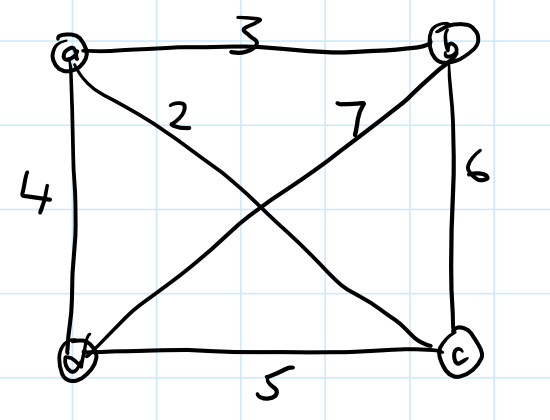
\includegraphics[]{matching_game_2.png}
	\end{figure}
\end{center}

We interpret the weight of an edge as the value generated by the two players on both sides when they work together. 

This game is superadditive, so we only need to consider the grand coalition when determining if it has a non-empty core. 

Recall: $((N), x)$ is in the core if and only if $x \in \mathcal{C}$ where $\mathcal{C} = \{x \in \mathbb{R}^N : x(N) = v(N), x(C) \geq v(C) \;\;\forall\; C \subseteq N\}$. 

There are exponentially many inequalities, but we can make a simplification. 

\begin{theorem}
	Let $\mathcal{C}' = \{x \in \mathbb{R}^N : x(N) = v(N), x_u + x_v \geq w_{uv} \;\; \forall \; uv \in E(G), x \geq \vec{0}\}$. We have $\mathcal{C}' = \mathcal{C}$
\end{theorem}

\begin{proof}
	If $x \in \mathcal{C}$, then $x$ satisfies all constraints in $\mathcal{C}'$ (we may take $C = \{u, v\}$ for each $uv \in E(G)$, and take $C = \{v\}$ to get $x \geq \vec{0}$). So $\mathcal{C} \subseteq \mathcal{C}'$
		
	Let $x \in \mathcal{C}'$. Then $x(N) = v(N)$. Let $C \subseteq N$, and let $M$ be a maximum weight matching in $C$. Our goal is to show that $x(C) \geq v(C) = w(M)$. Then \begin{align*}
	x(C) &\geq \sum_{uv \in M}x_u + x_v \text{ since }M \text{ is a matching, so no vertex repeated, and }x \geq \vec{0}\\
	&\geq \sum_{uv \in M} w_{uv} \text{ since } x \in \mathcal{C}'
	&= w(M) = v(C) 
	\end{align*}
\end{proof}

Here is an example of maximum matching with its payoff vector: 

\begin{center}
	\begin{figure}[h!]
		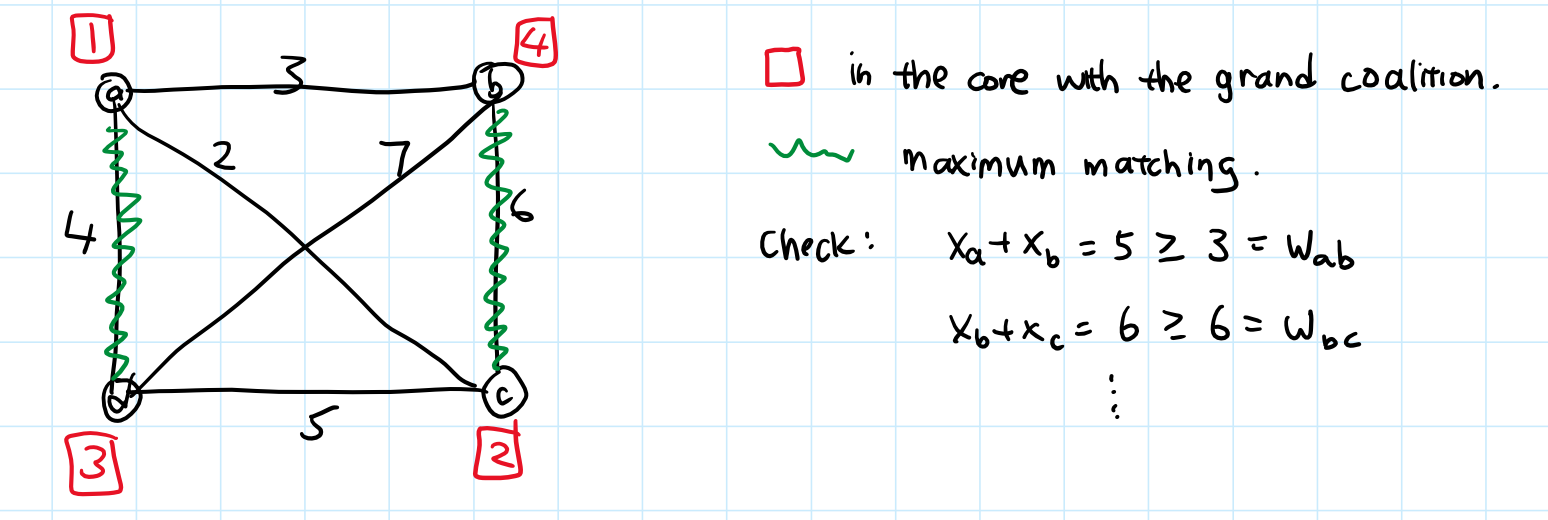
\includegraphics[width=\textwidth]{matching_game_3.png}
	\end{figure}
\end{center}

We can see that the edges in the maximum matching are ``efficient'', i.e. $$x_u + x_v = w_{uv}$$ for all $uv \in M$

In the example below, there are no outcomes in the core. We have $v(\{a, b, c\}) = 3$. If $((N), x)$ is in the core, then $x_a + x_c = 3$, which implies that $x_b = 0$. At least one of $x_a, x_c$ is at most 1.5, say it is $x_a$. Then $x_a + x_b \leq 1.5$, contradicting that $x_a + x_b \geq 2$. Hence, the core is empty. 

\begin{center}
	\begin{figure}[h!]
		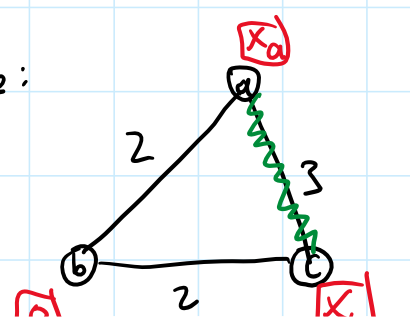
\includegraphics[]{matching_game_4.png}
	\end{figure}
\end{center}

We can determine if $\mathcal{C}'$ is empty by solving the following LP $(P)$: 

\begin{align*}
	\min              & \;\;\;x(N)                                              \\
	\text{ such that} & \;\;\;x_u + x_v \geq w_{uv} \;\; \forall \; uv \in E(G) \\
	                  & \;\;\; x\geq \vec{0}                                    
\end{align*}

For example, we have \begin{align*}
\min &\;\;\;x_a + x_b + x_c + x_d\\
\text{ such that} &\;\;\;x_a + x_b \geq 3\\
&\;\;\; x_a + x_c \geq 2\\
&\;\;\; x_a + x_d \geq 4\\
&\;\;\; \vdots\\
&\;\;\; x\geq \vec{0}
\end{align*}

$\mathcal{C}'$ is non-empty if and only if $(P)$ has optimal value $v(N)$. 

Taking the dual $(D)$, we get 

\begin{align*}
	\max              & \;\;\;\sum_{uv \in E(G)} w_{uv} y_{uv}                             \\
	\text{ such that} & \;\;\;\sum_{\{uv : uv \in E(G)\}}y_{uv} \leq 1 \;\;\forall u \in N \\
	                  & \;\;\; y\geq \vec{0}                                               
\end{align*}

For example, we have \begin{align*}
\max &\;\;\;3y_{ab} + 2y_{ac} + 4y_{ad} + \cdots\\
\text{ such that} &\;\;\;y_{ab} + y_{ac}+y_{ad} \leq 1
&\;\;\; \vdots\\
&\;\;\; y\geq \vec{0}
\end{align*}

Hence, $\mathcal{C}'$ is non-empty if and only if $(D)$ has optimal value $v(N)$. 

Meaning of $y$: If $y$ is integral, then its values are 0 or 1. For each vertex, the number of incident edges with value 1 is at most 1. So, the edges with value 1 form a matching. Maximizing integral solutions will give us the weight of a max matching, which is $v(N)$. But $y$ could be fractional. So, feasible solutions to $(D)$ are generalized matchings. 

We may have the following fractional matching labelled as blue circles. The maximum matching is labelled with curly green lines. $v(N) = 3$. The sum of weights of the fractional solution is $\frac{1}{2} \cdot 2 + \frac{1}{2} \cdot 2 + \frac{1}{2} \cdot 3 = \frac{7}{2} > 3$. So, the optimal value of $(D)$ is not $v(N)$, which implies that this game has an empty core. 

\begin{center}
	\begin{figure}[h!]
		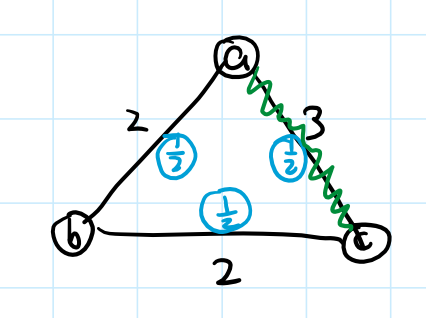
\includegraphics[]{matching_game_5.png}
	\end{figure}
\end{center}

\begin{theorem}
	The core of the matching game is non-empty if and only if $(D)$ has an integral optimal solution. 
\end{theorem}

\begin{proof}
	It suffices to prove that $(P)$ has optimal value $v(N)$ if and only if $(D)$ has an integral optimal solution. 
		
	$\Rightarrow$: Suppose $(P)$ has optimal value $v(N)$. Suppose $v(N) = w(M)$ for some maximum matching $M$. Define $y \in \mathbb{R}^{E(G)}$ by $y_e = \begin{dcases}
	0 & e \in M \\ 0 & e \notin M
	\end{dcases}$ for all $e \in E(G)$. Then $y$ is feasible for $(D)$ (since $M$ is a matching) with objective value $w(M) = v(N)$. By \textbf{Weak Duality Theorem}, $y$ is optimal for $(D)$, and it is an integral optimal solution. 
	
	$\Leftarrow$: Suppose $y$ is an integral optimal solution for $(D)$. Let $M' = \{e \in E(G) : y_e = 1\}$. Then $M'$ is a matching with optimal value $w(M')$. Since $y$ is optimal, $M'$ must be a maximum matching. So $w(M') = v(N)$. So $(P)$ has optimal value $v(N)$. 
\end{proof}

Note that when the graph is bipartite, $(D)$ always has an integral optimal solution. Hence, the core is non-empty. For general graphs, there is an efficient algorithm to determine if $(D)$ has an integral optimal solution. 

\section{Network Bargaining Game}

Two player bargaining: Suppose Alice and Bob are negotiating over how to split one million dollars. They can only take the money if both agree on how to split. 

Suppose there are outside options: Carol offers $\alpha$ to Alice if they work together, Dan offers $\beta$ to Bob if they work together. 

The result is as follows: 
\begin{center}
	\begin{figure}[h!]
		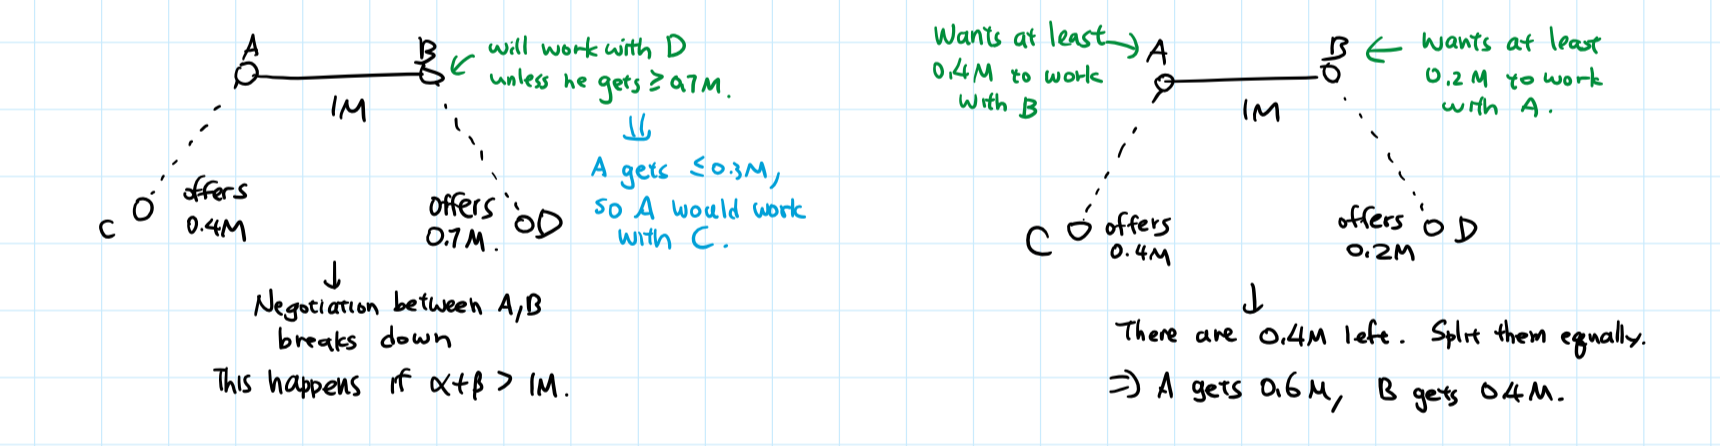
\includegraphics[width=\textwidth]{Network_Bargaining_game.png}
	\end{figure}
\end{center}

Nash's bargaining solution: Players $A, B$ try to split $w$, each has outside options $\alpha, \beta$ respectively. 

If $\alpha + \beta > w$, then no split is possible. Otherwise, $x_A = \alpha + \frac{w - \alpha - \beta}{2}$, $x_B = \beta + \frac{w - \alpha - \beta}{2}$

Given a graph $G$, the players are the vertices $N = V(G)$. Each edge $e$ has weight $w_e \geq 0$. Which pairs form? How do they split their value. 

In the example below, 5 players are negotiating. Who has more negotiating power? One possible result with partner (curly green line) and payoffs (red boxes). Player $b$ has the most powerful position. 
\newpage
\begin{center}
	\begin{figure}[h!]
		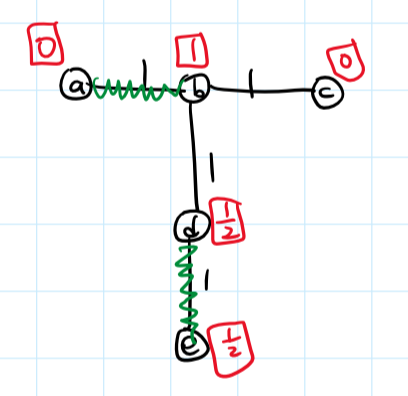
\includegraphics[]{Network_Bargaining_game_2.png}
	\end{figure}
\end{center}

An outcome of the network bargaining game consists of a matching $M$ and a payoff vector $x \in \mathbb{R}^N$ such that $x_u + x_v = w_{uv}$ for all $uv \in M$, $x_v = 0$ if $v$ is not matched by $M$, $x \geq \vec{0}$. 

The stability of an outcome depends on outside options of the players. 

\begin{definition}
	For an outcome $(M, x)$ and a player $u$, the \textbf{\underline{outside option}} of $u$ is $\alpha_u = \max ( \{0\} \cup \{w_{uv} - x_v : uv \in E \setminus M \})$. 
\end{definition}

This is the maximum value that $u$ can get by detecting from their current partner in $M$. No need to detect if $\alpha_u \leq x_u$. 

\begin{definition}
	An outcome $(M, x)$ is stable if $\alpha_u \leq x_u$ for all $u \in N$. 
\end{definition}

The example below shows a stable outcome: 
\newpage
\begin{center}
	\begin{figure}[h!]
		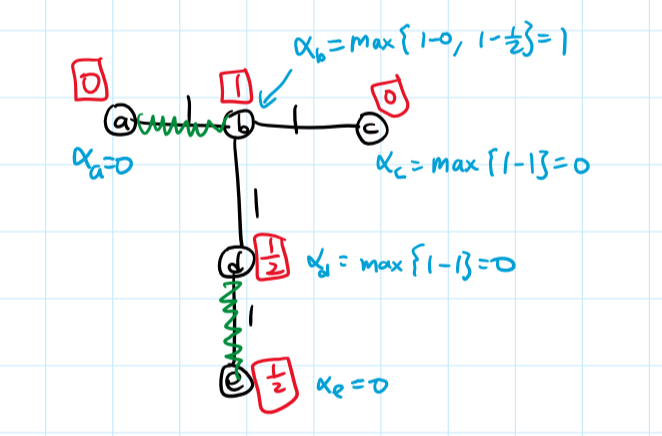
\includegraphics[]{Network_Bargaining_game_3.png}
	\end{figure}
\end{center}

To be stable, for each edge $uv$, $x_u \geq \alpha_u \geq w_{uv} - x_v$. So, $x_u + x_v \geq w_{uv}$. This is in $\mathcal{C}'$ from the matching game. 

\begin{theorem}
	A stable outcome exists in a network bargaining game if and only if the corresponding matching game has a non-empty core. 
\end{theorem}

However, a stable outcome might not reflect real life experimental results. 

For the example below, this is a stable outcome. In experiments, $b$ and $c$ tend to get more than $a$ and $d$. 

\begin{center}
	\begin{figure}[h!]
		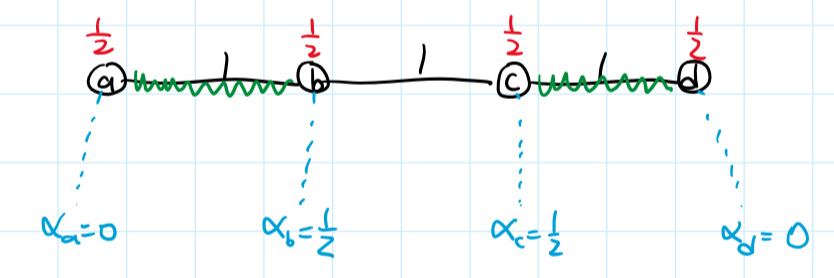
\includegraphics[width=\textwidth]{Network_Bargaining_game_4.png}
	\end{figure}
\end{center}

Idea from Nash's bargaining solution: In a matched pair, each player take at least their outside option and split the rest. In other words, after deducting their outside options, they are equal. 

\begin{definition}
	An outcome $(M, x)$ is \textbf{\underline{balanced}} if $x_u - \alpha_u = x_v - \alpha_v \geq 0$ for all $uv \in M$
\end{definition}

This is an example of a balanced outcome: 
\begin{center}
	\begin{figure}[h!]
		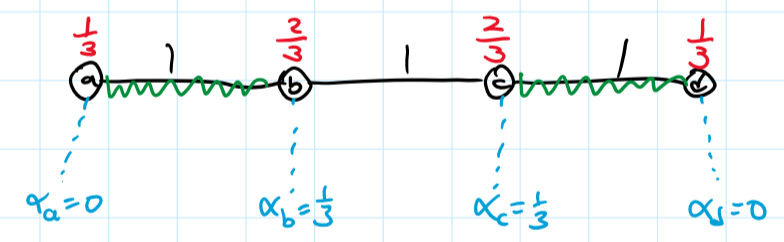
\includegraphics[width=\textwidth]{Network_Bargaining_game_5.png}
	\end{figure}
\end{center}

In the following example, $b$ is in a more powerful position: 
\begin{center}
	\begin{figure}[h!]
		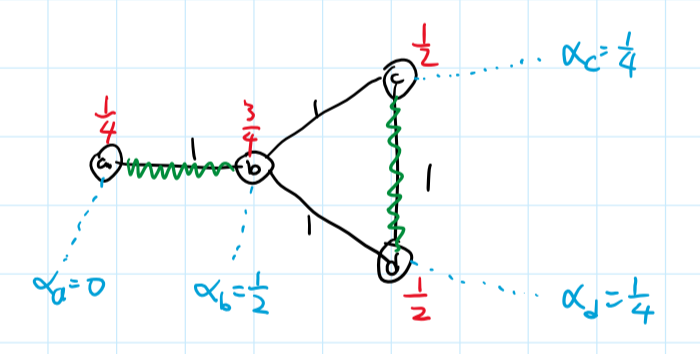
\includegraphics[width=\textwidth]{Network_Bargaining_game_6.png}
	\end{figure}
\end{center}

\begin{theorem}
	A network bargaining game has a balanced outcome if and only if it has a stable outcome
\end{theorem}

Note: It is not hard to prove that balanced outcomes are stable. 

\begin{definition}
	A vertex $v$ in a graph $G$ is essential if there exists a maximum matching in $G$ that does not use $v$. 
\end{definition}

For example, in the graph of a line with 3 vertices, $a, b$ and $c$. There are two maximum matchings. Either $a$ or $c$ is not used in the matchings. Hence, $a$ and $c$ are inessential. 

\begin{theorem}
	\textbf{Kleinberg and Tardos' Theorem}: In a graph $G$ with weight 1 for each edge, the following are equivalent: \begin{enumerate}
	\item There is a stable outcome
	\item There is a balanced outcome
	\item No two inessential vertices are adjacent
	\end{enumerate}
\end{theorem}

Aside: The set of inessential vertices is the set $D$ in the \textbf{Gallai-Edmonds Structure Theorem}. The third statement in the above theorem means that $D$ is independent. 


For general weights: we have 
\begin{theorem}
	\textbf{Kleinberg and Tardos' Theorem}: if a network bargaining game has a balanced outcome, then the balanced outcome must use the maximum weight matching, and there exists a polynomial time algorithm for finding a balanced outcome. 
\end{theorem}

\lecture{10}{November 17}{Martin Pei}{Haochen Wu}\\
This lecture's notes tend to be supplementary (add-on notes) of the course notes provided.
\section{Mechanism Design: Ideal Auctions}
Mechanism Design: we want to design games so that players are incentivized to achieve certain overall goals
\begin{example}
	Example of Mechanism Designs: \begin{enumerate}
	\item Elections: if more people prefer $A$ over $B$, then $A$ should win
	\item Auctions: the player who values the item the most should win. Or, maximize revenue for the seller.
	\item Sports Tournaments: best team should win, team play the best they can. 
	\end{enumerate}
\end{example}
However, there could be problems: people look after themselves, and will find loopholes and advantages to avoid playing as the game designer intended. 

The main questions is: How to set rules so that players who play for themselves will also achieve these global goals? 

In an auction, the auctioneer is selling something, and players bid on the item. Auctioneer needs to decide the rules for two things: who wins what item, and who pays what amount. In the case of second price auction, player who bids the most wins, and the winner pays second highest bid. 

There are a bunch of nice properties of second-price auctions: \begin{itemize}
\item Recall that a player bidding their valuation is a dominant strategy. This makes them tend to make ``truthful bidding''. 
	
This is easy to play: even without knowing everyone else's valuation, bidding one's own valuation will maximize utility. 
	
However, truthful bidding is not a dominant strategy for the first-price auction. 
	
\item If players give truthful bids, then their utility is never negative. This is not true for ``all-pay'' auction, where every player pays regardless if they win or lose. 
\end{itemize}

\begin{definition}
	An auction is \textbf{\underline{dominant-strategy incentive-compatible (DSIC)}} if truthful bidding is a dominant strategy, and yields non-negative utility. 
		
	Note that dominant strategy here means ``weakly dominant'' except we don't require a case that decrease utility. 
\end{definition}

Having DSIC is not good enough. For example, an auction where we give the item for free to player 1 is DSIC. 

We need an overall goal: the item should go to the player with the highest valuation. Here is the notion of ``social welfare'': it is the sum total of values received by all players. 

For one-item auctions, only one player receives the item. If player $i$ wins the auction, then they receive value $v_i$ (their valuation). Remaining players receives nothing. So, the social welfare is $v_i$. 

To maximize the social welfare in this case, we just make sure that the player with the highest valuation wins. This is easy if players bid truthfully. 

\begin{definition}
	An auction is ``welfare-maximizing'' if truthful bidding results in maximum social welfare. 
\end{definition}

Last good property for second-price auction is that it is easy to run. We can quickly determine the highest bidder and the second highest bid. 

\begin{definition}
	An auction is ideal if: \begin{enumerate}
	\item It is DSIC
	\item It is welfare-maximizing
	\item It can be implemented efficiently
	\end{enumerate}
\end{definition}

\begin{theorem}
	The second-price auction is ideal
\end{theorem}

We may also know that this is the only single-item auction that is ideal. 

\section{Sponsored Search Auctions}
Search engines may show ads as the first entries of a search result. Selecting which ads to show and their order of placement is done through auctions. 

Here is how we model this problem. 

Suppose there are $k \geq 1$ slots for sponsored links on a search results page. There are advertisers $N$ bidding for these slots with related keywords. The slots have different ``values'': top ones tend to get clicked more often. We have ``click through rate'', known as CTR, for each slot. For each slot $j$, let $\alpha_j \in [0, 1]$ be the probability that a user clicks on an ad at slot $j$. 

First, we assume that $\alpha_1 \geq \alpha_2 \geq \alpha_3 \geq \cdots$

Second, we assume that CTR is independent of the quality of the ad.

We are looking for ideal auctions, which should be DSIC, welfare-maximizing, and efficient. We need to determine who wins what, and who pays what. 

The general approach is \begin{enumerate}
\item Assume truthful bidding, how can we assign the items that is welfare-maximizing and efficient? 
\item Given the way we assign items, how can we set prices so that it is DSIC? 
\end{enumerate}

In terms of social welfare, we want to maximize the overall value for the players. What is the value to a player? Each player $i$ has a valuation $v_i$ of how much one click on their ad is worth. 

If they are assigned a slot with CTR $x_i$, then their expected value is $v_ix_i$. The social welfare is $\sum_{i \in N} v_ix_i$. 

What is a rule that maximizes the social welfare? We should be assigning slot 1 to the player with the highest valuation, slot 2 to the second highest, etc. This can be efficiently implemented as well. 

It is worth to note that efficiency is critical. Lots of sponsored search auctions run at the same time. It has to be almost instantaneous. 

In terms of payment rules, we want it to be DSIC, so that players are incentivized to bid truthfully. This requires Myerson's Lemma. 

Consider the genralized second-price auction. The player who wins the $j$-th slot will pay $(j+1)$-th highest bid times their CTR $\alpha_j$. This is not DSIC. 

\begin{example}
	Let's say there are 2 slots and 3 players. Let the CTRs be $\alpha_1 = 0.7, \alpha_2 = 0.5$. Player valuations are $v_1 = 10, v_2 = 9, v_3 = 2$. 
		
	If we assign slot 1 to player 3 and slot 2 to player 1, then the social welfare i $10 \times 0.5 + 0 + 2 \times 0.7 = 6.4$. 
		
	If we apply the rules for generalized second-price auction, we can see that payment rule is not DSIC. 
		
	In this case, player 1 gets CTR $\alpha_1$, and gets value $v_1\alpha_1 = 7$. Their payment is $v_2\alpha_1 = 6.3$. The utility is 0.7. However, if player 1 bids 8 instead, then they will get CTR $\alpha_2$, and value $v_1\alpha_2 = 5$. Their payment is $v_3\alpha_2 = 1$. The utility is 4. 
		
	Hence, truthful bidding is not a dominant strategy. 
\end{example}

\section{Myerson's Lemma}
Myerson's Lemma characterizes auctions that have $DSIC$ payment rule, and gives a formula for the payment rule. 

We first need an abstraction of the auction model. 

\begin{definition}
	In a \textbf{\underline{single-parameter environment}}, we are given: \begin{itemize}
	\item A set of players $N$
	\item A private valuation $v_i \geq 0$ for each $i \in N$, which is player $i$'s valuation for one unit of goods. 
	\item A set $X \subseteq \mathbb{R}^N$ of vectors $(x_1, ..., x_n)$ that describe feasible allocations, i.e. $x_i$ is the amount of goods given to player $i$. 
	\end{itemize}
\end{definition}

Note that this is ``single-parameter'' since each player has only one piece of private information. 

\begin{example}
	In a single-item auction, $X$ is the set of all standard basis vectors in $\mathbb{R}^n$ ($n$-tuples with one 1 and $n-1$ 0's). 
		
	In the sponsored search auction, $X$ is the set of vectors where for each slot $j$, at most one $i \in N$ satisfies $x_i = \alpha_j$, and $0$ otherwise. 
\end{example}

We are interested in mechanisms in this environment, i.e. the rules of the auction. Let $B \subseteq \mathbb{R}^N$ be the set of all possible player bids. 

\begin{definition}
	Given a single-parameter environment, a \textbf{\underline{direct revelation mechanism}}: \begin{itemize}
	\item collects bids $b \in B$ from all players
	\item choose a feasible allocation $x(b) \in X$ based on the bids
	\item choose a payment $p(b) \in \mathbb{R}^N$ where player $i$ pays $p_i(b)$
	\end{itemize}
	We call $x: B \rightarrow X$ an \textbf{\underline{allocation rule}}, and $p: B \rightarrow \mathbb{R}^N$ a \textbf{\underline{payment rule}}. The utility of player $i$ is $u_i(b) = v_ix_i(b) - p_i(b)$
	
	As part of the DSIC condition, we assume $0 \leq p_i(b) \leq v_ix_i(b)$, i.e. truthful bidding will result in non-negative utility. 
\end{definition}

\begin{example}
	For the second-price auction, $$x_i(b)  = \begin{dcases}
	1 & b_i \text{ is max in } b\\ 0 & \text{otherwise}
	\end{dcases}$$ and $$p_i(b) = \begin{dcases}
	\max_{j \neq i} b_j & b_i \text{ is max in } b\\ 0 & \text{otherwise}
	\end{dcases}$$
\end{example}

\begin{definition}
	There are two terms for an allocation rule\begin{enumerate}
	\item An allocation rule $x: B \rightarrow X$ is \textbf{\underline{implementable}} if there exists a payment rule $p: B \rightarrow \mathbb{R}^N$ such that $(x, p)$ is DSIC. The single-item auction where we give the item to the highest bidder is implementable, by using the second-price rule as payment. 
	\item An allocation rule $x: B \rightarrow X$ is \textbf{\underline{monotone}} if for all $i \in N$ and for all $b_{-i} \in B_{-i}$, $x_i(z, b_{-i}) \geq x_i(y, b_{-i})$ whenever $z \geq y$, i.e. the higher you bid, the more you get. 
		
	For single-item auctions, highest bid wins is monotone. But second highest bid wins is not monotone (you can lose things by bidding higher)
	\end{enumerate}
\end{definition}

The main is result is as follows: 
\begin{theorem}
	\textbf{Myerson's Lemma}: For a single parameter environment, an allocation rule $x: B \rightarrow X$ is implementable if and only if $x$ is monotone. Moreover, given a monotone allocation rule $x : B \rightarrow X$, there exists a unique payment rule $p: B \rightarrow \mathbb{R}^N$ such that $(x, p)$ is DSIC and $p_i(b) = 0$ whenever $b_i = 0$. 
\end{theorem}

\lecture{11}{November 24}{Martin Pei}{Haochen Wu}\\
This lecture's notes tend to be supplementary (add-on notes) of the course notes provided.
\begin{lemma}
	If an allocation rule $x: B \rightarrow X$ is implementable, then $x$ is monotone. 
\end{lemma}
\begin{proof}
	Suppose $x$ is implementable, then there exists a payment rule $p: B \rightarrow \mathbb{R}^n$ such that $(x, p)$ is $DSIC$. 
		
	Fix a player $i \in N$, and bids $b_{-i} \in B_{-in}$. We use $x(y), p(y)$ to represent $x_i(y, b_{-i})$ and $p_i(y, b_{-i})$ to simplify the notation. 
		
	We want to prove that if $y \geq z$, then $x(y) \geq x(z)$. Let's assume $y \geq z$. The key observation is that the rules $(x, p)$ are defined independent of the players' evaluations. 
		
	\begin{enumerate}
		\item $(x, p)$ is DSIC if player $i$'s valuation is $y$. So utility of bidding $y$ $\geq$ utility of bidding $z$. 
		      		
		      This gives us $y \cdot x(y) - p(y) \geq y \cdot x(z) - p(z)$
		\item $(x, p)$ is DSIC if player $i$'s valuation is $z$. So utility of bidding $z$ $\geq$ utility of bidding $y$. 
		      		
		      This gives us $z\cdot x(z) \geq z \cdot x(y) - p(y)$. 
	\end{enumerate}
	Rearranging the inequalities, we can get $$z(x(y) - x(z)) \leq p(y) - p(z) \leq y(x(y) - x(z))$$
	This is known as \textbf{Payment Sandwich}. Since $y \geq z \geq 0$, we have $x(y) - x(z) \geq 0$. So, $x(y) \geq x(z)$. 
\end{proof}

The above gives the proof for one side. We prove the other side by breaking it down to a few lemmas (we only prove the case when $x$ is piecewise constant). 

The general approach is: assume $x$ is monotone, and $(x, p)$ is DSIC. Derive that $p$ is unique with $p_i(b) = 0$ whenever $b_i = 0$. Then, we prove that using this particular $p$, $(x, p)$ is indeed DSIC. 

We can describe a generic $x$ that is monotone and piecewise constant. There are jump points $\bar{z}_1 < \bar{z}_2 < \cdots < \bar{z}_q$ as shown below. 
\newpage
\begin{center}
	\begin{figure}[h!]
		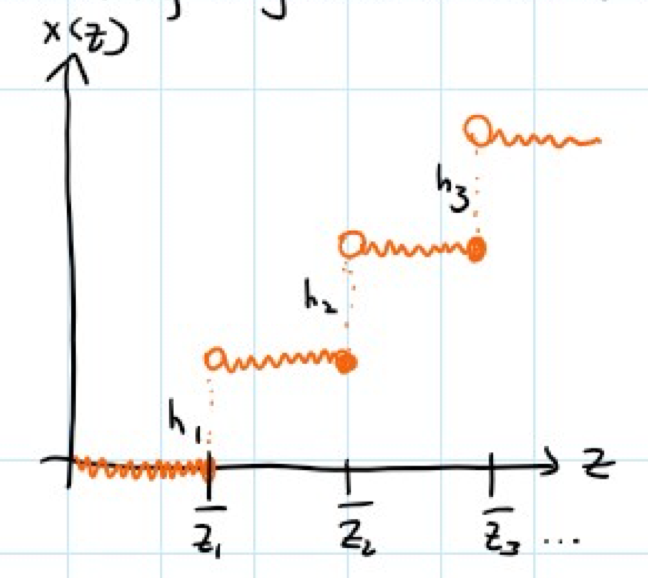
\includegraphics[width=.5\textwidth]{myerson.png}
	\end{figure}
\end{center}

We can see that $x$ is constant in the intervals $[0, \bar{z}_1], (\bar{z}_1, \bar{z}_2], ..., (\bar{z}_{q-1}, \bar{z}_{q}], (\bar{z}_q, \infty)$
	
	\begin{lemma}
		If $x$ is monotone and piecewise constant, and $(x, p)$ is DSIC with $p_i(b) = 0$ whenever $b_i = 0$, then $p$ is unique
	\end{lemma}
	\begin{proof}
		Assume $y > z$. Suppose $z \in (\bar{z}_j, \bar{z}_{j+1})$ for some $j$. We assume DSIC, so the payment sandwich applies. Divide by $y-z$ to get $$z \frac{x(y) - x(z)}{y-z} \leq \frac{p(y) - p(z)}{y-z} \leq y \frac{x(y) - x(z)}{y-z}$$
			
		Take the limit as $y \rightarrow z^+$, we have $\lim\limits_{y\rightarrow z^+} \frac{x(y) - x(z)}{y-z} = x'(z) = 0$ since $x$ is constant at $z$. 
			
		So both ends of the inequalities approach 0. By \textbf{Squeeze Theorem}, $\lim\limits_{y\rightarrow z^+} \frac{p(y) - p(z)}{y-z} = p'(z) = 0$. 
			
		So, $p$ is piecewise constant with jumps at $\bar{z}_1, ..., \bar{z}_q$. Let $z = \bar{z}_j$ for some $j$. Look at the payment sandwich. We have $\lim\limits_{y\rightarrow z^+} y(x(y) - x(z)) = z \cdot h_j$, and $\lim\limits_{y\rightarrow z^+}z(x(y) - x(z)) = z \cdot h_j$. By \textbf{Squeeze Theorem}, $\lim\limits_{y\rightarrow z^+} p(y) - p(z) = z \cdot h_j = z_j \cdot h_j$. So, the payment jump at $\bar{z}_j$ is $\bar{z}_j h_j$. 
			
		By assumption, $p(0) = 0$. This gives us the starting point. This uniquely defines the function $p$: If $j$ is the largest index where $z \geq \bar{z}_j$, then $$p(z) = p_i(z, b_{-i}) = \sum_{k=1}^{j}\bar{z}_kh_k$$
	\end{proof}
	
	Let's visualize this payment rule. The payment is the area to the ``left'' of $x$. 
	
	\begin{center}
		\begin{figure}[h!]
			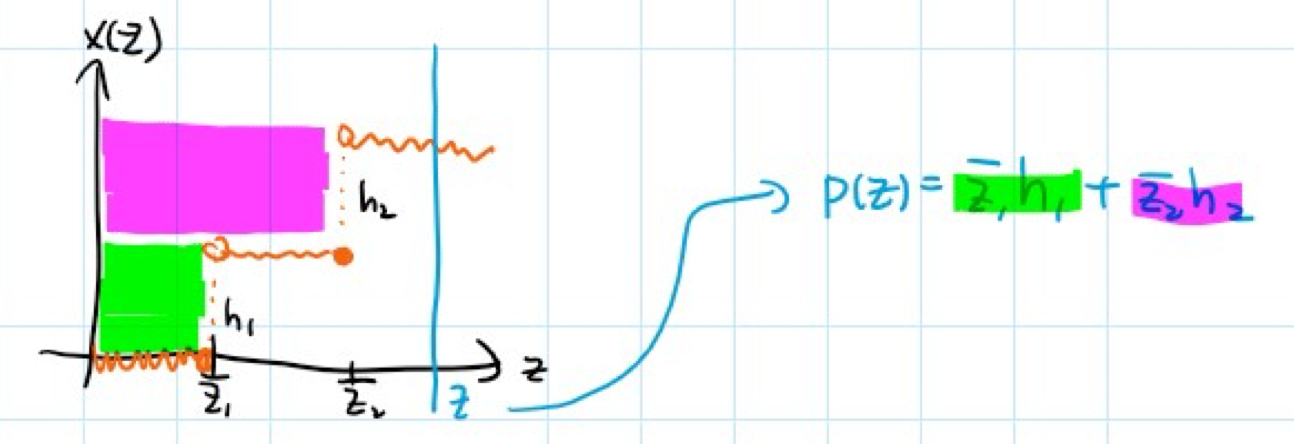
\includegraphics[width=.7\textwidth]{myerson_2.png}
		\end{figure}
	\end{center}
	
	\begin{lemma}
		The payment rule $p$ from \textbf{Lemma 11.181} is DSIC. 
	\end{lemma}
	
	The proof is by visualizing it in a picture. 
	
	\begin{center}
		\begin{figure}[h!]
			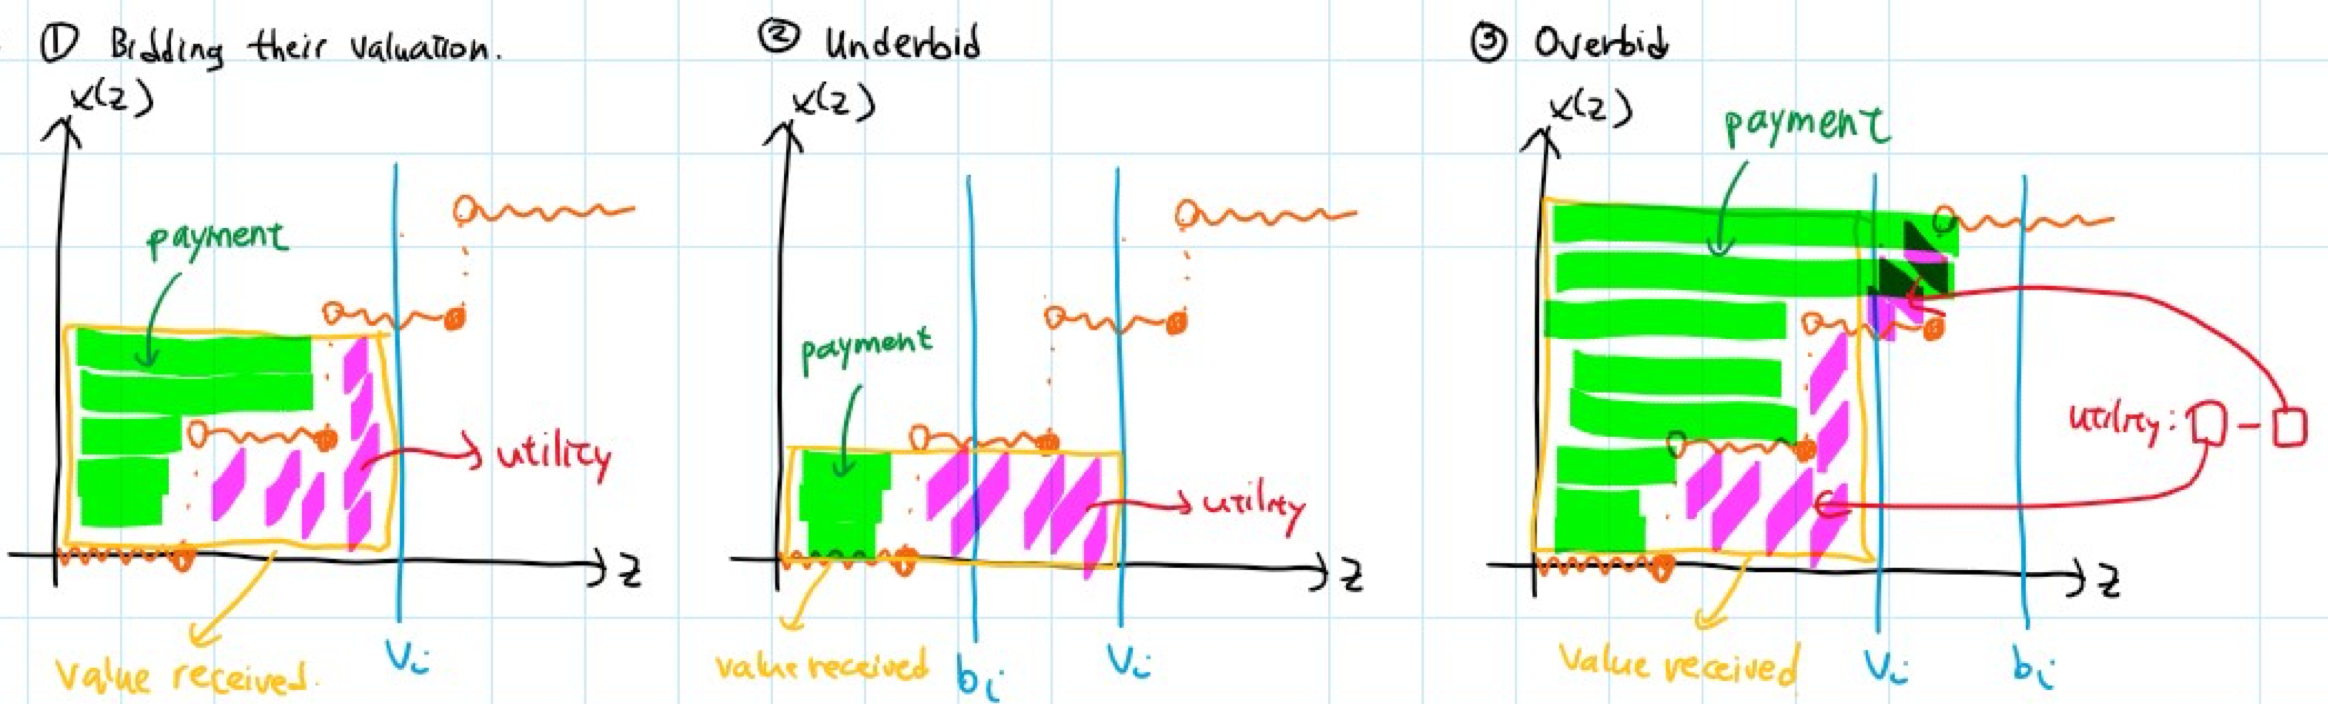
\includegraphics[width=\textwidth]{myerson_3.png}
		\end{figure}
	\end{center}
	
	The utilities for underbid and overbid are at most the utility of bidding at valuation. Also, the utility of truthful bidding is non-negative. So, this payment is DSIC. 
	
	\section{Applying Myerson's Lemma}
	Recall that the payment rule is $p_i(z, b_{-i}) = \sum_{k=1}^{j}\bar{z}_kh_k$. 
	
	\begin{enumerate}
		\item In a single item auction, let $x$ be the allocation rule that gives the item to the highest bidder (with a consistent tie-breaking rule). This is monotone. Consider a player $i$ and bids $b_{-i} \in B_{-i}$. Let $B = \max_{j \neq i} b_j$. 
		      The allocation function for player $i$ is as follows: 
		      \begin{center}
		      	\begin{figure}[h!]
		      		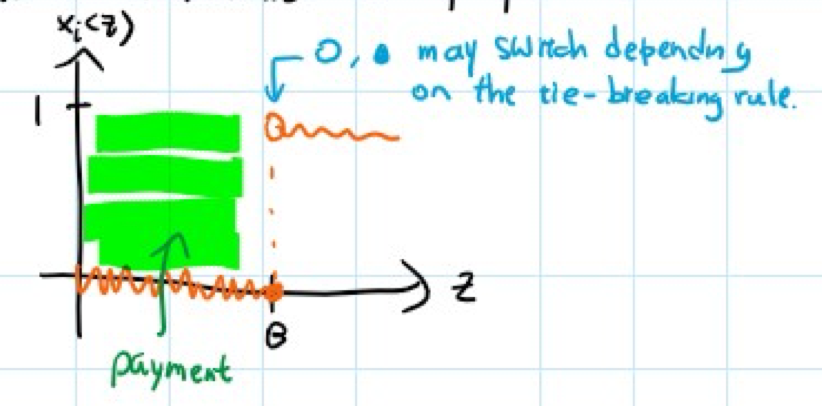
\includegraphics[width=.7\textwidth]{myerson_4.png}
		      	\end{figure}
		      \end{center}
		      There is one jump at $z = B$. When $b_i > B$, player $i$ wins and the payment is $B \cdot 1 = B$. This is second-price rule, and it is unique assuming $b_i = 0$ implies $p_i = 0$. 
		\item Sponsored search auction. There are $k$ slots with CTR $\alpha_1 \geq \alpha_2 \geq \cdots \geq \alpha_k$. Out allocation function $x$ assigns $\alpha_j$ to the $j$-th highest bidder. This is monotone. Let's apply Myerson's lemma for the payment rule. 
		      
		      Consider a plyaer $i$ and bids $b_{-i} \in B_{-i}$. Assume $b_1 \geq b_2 \geq \cdots \geq b_k$ (ignore the rest). Player $i$ gets $\alpha_k$ if $b_k < b_i \leq b_{k-1}$, and gets $\alpha_{k-1}$ if $b_{k-1} < b_i \leq b_{k-2}$, etc. The graph is as follows: 
		      \begin{center}
		      	\begin{figure}[h!]
		      		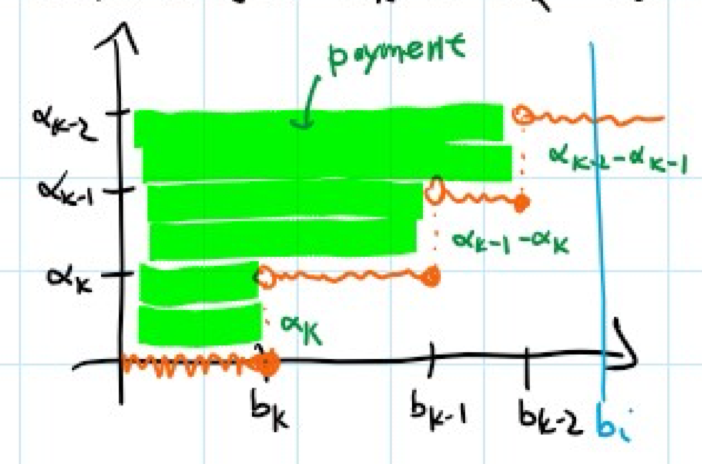
\includegraphics[width=.5\textwidth]{myerson_5.png}
		      	\end{figure}
		      \end{center}
		      Each jump is $\alpha_{j-1} - \alpha_j$. Using the formula, $p_i(z) = \sum_{\{j : b_j < 2\}} b_j(\alpha_j - \alpha_{j+1})$ using $\alpha_{k+1} = 0$. This is the unique DSIC payment rule.
		      
		      For example,
		      \begin{center}
		      	\begin{figure}[h!]
		      		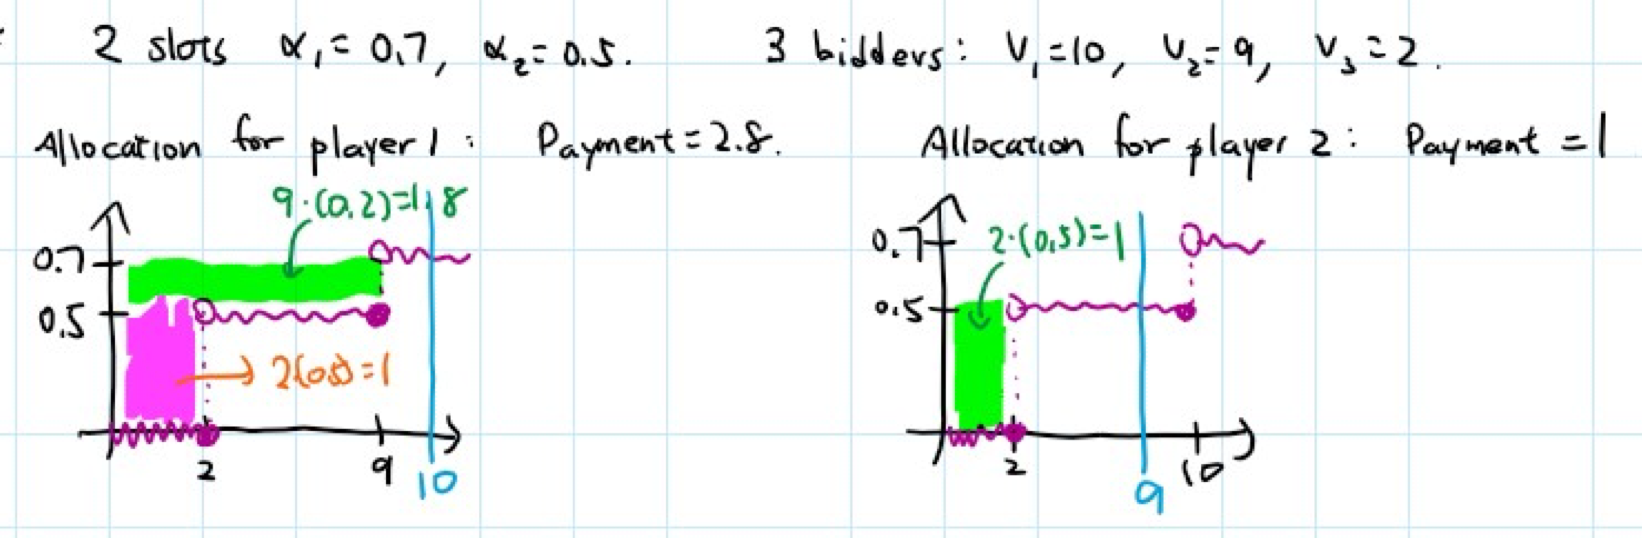
\includegraphics[width=\textwidth]{myerson_6.png}
		      	\end{figure}
		      \end{center}
	\end{enumerate}
	
	\section{Knapsack Auction}
	An ideal auction is DSIC, welfare-maximizing, and efficient. We consider an auction that cannot be ideal. 
	
	We are managing advertising slots for a TV station. We have $T$ seconds to fill. There are potential advertisers $N$. Advertiser $i$ has an ad of length $t_i$ and gets a value of $v_i$. We run auction to determine whose ads to air. 
	
	Here is an example: 
	\begin{center}
		\begin{figure}[h!]
			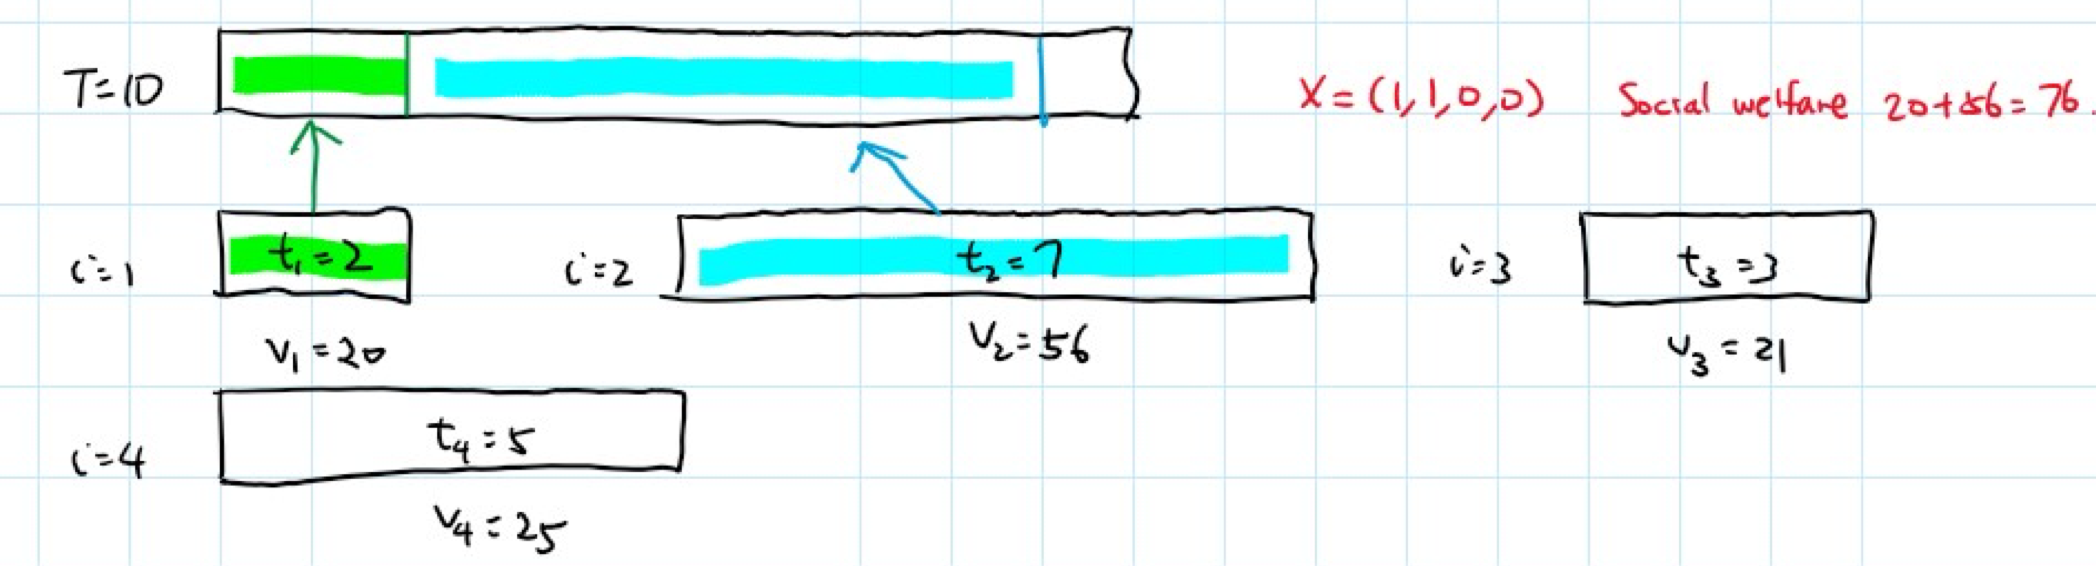
\includegraphics[width=\textwidth]{knapsack.png}
		\end{figure}
	\end{center}
	
	The set of feasible solutiions are $X = \{x \in \{0, 1\}^N : \sum_{i \in N} t_i x_i \leq T\}$, social welfare is $\sum_{i \in N} v_ix_i$. To maximize welfare, we need $\max \{v^Tx : x \in X\}$. 
	
	Recall that the first stage of designing this auction is to assume players bid truthfully, and find an allocation rule that is welfar-maximizing. Then, Myerson's lemma gives us a payment rule that is DSIC. 
	
	However, the problem is that, maximizing social welfare is equivalent to the knapsack problem. This is NP-hard, so it is not possible to find an optimal solution efficiently (unless $P = NP$). We cannot maximize social welfare and get a solution efficiently simultaneously. 
	
	The solution is that, we relax either constraints. We need to have an efficient solution since it has to be practical, which is to be run at real-time. So, instead of finding a welfare-maximizing allocation, we will find an approximation of the allocation that is ``close'' to maximum, while keeping efficiency. 
	
	\lecture{12}{December 1}{Martin Pei}{Haochen Wu}\\
	This lecture's notes tend to be supplementary (add-on notes) of the course notes provided.
	
	\section{Knapsack auction}
	Our goal is to approximate the welfare-maximizing function for the knapsack auction. 
	
	Typically with approximation algorithms, we want some preference guarantee, i.e. we want ``the solution produced by the algorithm must be at least this close to the theoretical optimal''
	
	For example, we have \begin{center}
	\begin{tabular}{|c|c|c|c|c|}
		\hline
		$i$         & 1  & 2  & 3  & 4  \\
		\hline
		$t_i$       & 2  & 7  & 3  & 5  \\
		\hline
		$v_i$       & 20 & 56 & 21 & 25 \\
		\hline
		$v_i / t_i$ & 10 & 8  & 7  & 5  \\
		\hline
	\end{tabular}
	\end{center}
	The idea is that, we have limited space, so we want to fill in each unit with as much value as possible. This leads us to calculate the value density. Higher density should give better value. We sort items in non-increasing value density, i.e. $\frac{v_1}{t_1} \geq \frac{v_2}{t_2} \geq \cdots \geq \frac{v_n}{t_n}$. 
	
	First, we try to puck items $1, 2, ...$ until we cannot put the next one in the kanpsack.
	
	In the example above, we pick $1$ and $2$, and we have $t_1 + t_2 = 9 \leq 10$, there is no room for 3. The total value is 76. 
	
	However, there are cases where such algorithm gives very bad solution. 
	
	For example, there are two players $v_1 = t_1 = 1$, and $v_2 = T - 1, t_2 = T$. 1 has higher density than 2. If we pick 1, then we do not have room for 2. The value produced by this algorithm is 1. The obvious optimal solution is to pick 2, which gives the optimal value of $T - 1$. Our solution is $\frac{1}{T - 1}$ of the optimal. 
	
	A better idea could be: suppose we stop at item $i$ above. We check that the value of item $i+1$. If $v_{i+1} > \sum_{j = 1}^{i} v_i$, then we will say $i+1$ is the only winner. We assumed that $t_i \leq T$ for all $i$. 
	
	In the example above, we would pick 2 instead, which gives a better solution. 
	
	The full algorithm is that: Assume $N = \{1, ..., n\}$ with $\frac{v_1}{t_1} \geq \frac{v_2}{t_2} \geq \cdots \geq \frac{v_n}{t_n}$: \begin{itemize}
	\item Find $i$ such that it is the largest index with $t_1 + \cdots + t_i \leq T$
	\item If $v_1 + \cdots + v_i \geq v_{i+1}$, then $\{1, ..., i\}$ are the winners. Otherwise, $\{i+1\}$ is the only winner. 
	\end{itemize}
	
	\begin{theorem}
		$APX \geq \frac{1}{2} OPT$. This means that the solution produced by the approximated algorithm is guaranteed to be at least halfway to the optimal. 
	\end{theorem}
	\begin{proof}
		A welfare-maximizing solution is optimal for this integer program $(IP)$: $$\max \{\underbrace{v^Tx}_{sum of the values} : \underbrace{t^Tx \leq T}_{fit into the knapsack},  x_i \in \{0, 1\} \text{ for all }i\}$$The optimal value is OPT. 
			
		Its LP relaxation $(LP)$ is $$\max \{\underbrace{v^Tx}_{sum of the values} : \underbrace{t^Tx \leq T}_{fit into the knapsack},  0 \leq x_i \leq 1\text{ for all }i\}$$ this means that the solutions can be fractional. 
			
		Let $i$ be the largest index with $t_1 + \cdots + t_i \leq T$. Consider the solution $x$ where $$x_1 = \cdots = x_i = 1, x_{i+1} = \frac{T - t_1 - \cdots - t_i}{t_{i+1}}, x_{i+2} = \cdots = x_n = 0$$
		The idea is essentially filling in the remaining space with a fraction of item $i+1$. In the example above, we would have $x_1 = x_2 = 1, x_3 = \frac{1}{3}, x_4 = 0$. 
			
		As we completedly filled in the knapsack with the highest-density items, $x$ is optimal. 
			
		Exercise: Prove that $x$ is optimal formally using duality. 
			
		Suppose optimal value of (LP) is $v^*$, obtained by $x$. Since (LP) is a relaxation of (IP), we have $OPT \leq v^*$. 
			
		We want to prove that $APX \geq \frac{v^*}{2}$. 
			
		Let $S = \{1, ..., i\}$. We see that $v^* \leq v_1 + \cdots + v_i + v_{i+1} = v(S) + v_{i+1}$. There are two cases: \begin{itemize}
		\item If $v(S) \geq v_{i+1}$, then the algorithm picks $S$, so $APX = v(S)$. Then $v^* \leq v(S) + v_{i+1} \leq v(S) + v(S) = 2APX$
		\item If $v(S) < v_{i+1}$, then the algorithm picks $\{i+1\}$, so $APX = v_{i+1}$. Then, $v^* \leq v(S) + v_{i+1} \leq 2v_{i+1}= 2APX$
		\end{itemize}
		
		So, $APX \geq \frac{v^*}{2} \geq \frac{1}{2}OPT$
			
	\end{proof}
	
	Exercise: prove that the allocation rule derived from the approximation is monotone. 
	
	Myerson's lemma gives a payment rul for our allocation. A player either wins or not. So the allocation function looks like 
	\begin{center}
		\begin{figure}[h!]
			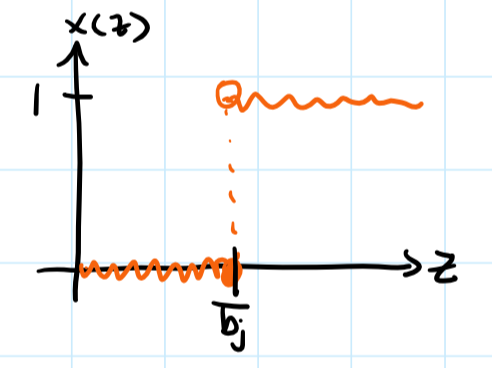
\includegraphics[width=.5\textwidth]{knapsack_2.png}
		\end{figure}
	\end{center}
	Say this is for player $j$, and the jump occurs at $\bar{b}_j$. The payment for winning is then $\bar{b}_j$. How do we find $\bar{b}_j$? Maybe use binary search, or use some logic. 
	
	\begin{example}
		Using the following example again: \begin{center}
		\begin{tabular}{|c|c|c|c|c|}
			\hline
			$i$         & 1  & 2  & 3  & 4  \\
			\hline
			$t_i$       & 2  & 7  & 3  & 5  \\
			\hline
			$v_i$       & 20 & 56 & 21 & 25 \\
			\hline
			$v_i / t_i$ & 10 & 8  & 7  & 5  \\
			\hline
		\end{tabular}
		\end{center}
		Approximation algorithm picks 1 and 2 as winners. What is the payment for player 2? The allocation is monotone, so to find $\bar{b}_2$, we need to lower $v_2$ until the approximation algorithm does not pick player 2. 
		
		As long as $\frac{v_2}{t_2} \geq 7$, the algorithm will pick 2. So, player 2 can go as low as 49. 
		
		What happens if $v_2$ goes below 49? Say it has value density $\geq 5$. The approximation algorithm will pick 1 and 3 with combined value 41, then look at $v_2$. If $v_2 \geq 41$, then the algorithm will still pick 2. If $v_2 \leq 41$, then the algorithm will stick with $1, 3$. So, $\bar{b}_2 = 41$, and the payment is 41. 
	\end{example}
	
	\section{Voting Mechanism}
	Voting: we want the result to represent the will of people. If there are 2 candidates, this is easy, and we may decide on majority. If there are 3 or more candidates, there would be a problem. 
	
	Condorcet's paradox: Let's say there are 3 candidates $a, b, c$: \begin{itemize}
	\item voter 1: $a >_1 b >_1 c$
	\item voter 2: $b >_2 c >_2 a$
	\item voter 3: $c >_3 a >_3 b$
	\end{itemize}
	A majority of voters prefer $a$ over $b$, $b$ over $c$, and $c$ over $a$. This gives $a > b > c >a$, but this is not possible. 
	
	If we only choose 1 candidate, then a majority wants a different one. 
	
	Thie could lead to ``strategic voting'': a voter may be incentivized to not vote for their preferred candidate. 
	
	\begin{example}
		$a, b$ are front runners, more prefer $a$ over $b$. A group of voters prefers $c$, who has no chance of winning. But they would rather $b$ win than $a$. So, they vote for $b$ instead. 
	\end{example}
	
	The problem is that: the usual voting mechanism does not incentivize voters to vote truthfully. So the votes that are submitted do not represent the will of the people. 
	
	Is there a voting mechanism where truthful voting is a dominant strategy? The answer is No, if we want our voting mechanism to have the obvious good properties. 
	
	\begin{definition}
		Set up of the model: There is a group of candidates $A$, voters $\{1, ..., n\}$. Let $L$ be the set of all total orders on $A$ (A total order is a relation $<$ on $A$ that is antisymmetic and transitive). 
			
		Antisymmetic means that, if $a \neq b$, then $a > b$ or $b>a$ (can't be both). 
			
		Transitive means that, if $a > b, b> c$, then $a > c$. 
			
		Each voter $i$ has a total order of preferences $<_i \in L$. $a <_i b$ means that voter $i$ prefers $b$ over $a$. 
			
		A collection of all voter prefereces $(<_1, ..., <_n) \in L^n$. 
			
		Given a collection of voter preferences (how voters should vote), there are 2 outcomes that may be generated by a voting mechanism: \begin{itemize}
		\item A \textbf{\underline{social welfare function}}: will output another total order on $A$ that represens ``society's preference'' $F : L^n \rightarrow L$. 
		\item A \textbf{\underline{social choice function}}: will output one candidate from $A$ that represents ``society's choice'' $f : L^n \rightarrow A$. 
		\end{itemize}
	\end{definition}
	
	Let $F: L^n \rightarrow L$, $(<_1, ..., <_n) \in L^n$. Suppose $F(<_1, ..., <_n) = <_1$. Here are the properties of a social welfare function: \begin{itemize}
	\item Good property 1: \textbf{Unanimity}. If every voter prefers $a$ over $b$, then the society prefers $a$ over $b$. (if $b <_i a$ for all $i \in N$, then $b < a$ in $F$). 
		
	\item Good property 2: \textbf{Independence of irrelevant alternatives (IIA)}. The society's preference between two candidates should only depend on the individual voters' preferences of these two candidates, and not on others. 
		
	Suppose $(<_1, ..., <_n), (<'_1, ..., <'_n) \in L^n$. $F(<_1, ..., <_n) = <$, $F(<'_1, ..., <'_n) = <'$. For two candidates $a, b \in A$, $a <_i b \Leftrightarrow a <'_i b$ (the relative rank of $a, b$ does not change between $<_i$ and $<'_i$) implies $a < b \Leftrightarrow a <' b$ (the relative rank of $a, b$ for $F$ does not change from $<$ to $<'$). 
		
	For example, suppose you can choose between studying game theory and cryptography. Of course you would choose game theory. Now, you have the additional option of studying Galois theory, and you decide to study cryptography instead. This should not happen. 
		
	\item Bad property 1: Dictorship. The society's prefernce completely agees with one particular voter's preferences in all cases, i.e. for all $(<_i, ..., <_n) \in L^n$, we have $F(<_1, ..., <_n) = <_i$. 
		
	\end{itemize}
	
	\begin{theorem}
		\textbf{Arrow's Impossibility Theorem}: Every social welfare function over a set of at least 3 candidates that satisfies ananimity and IIA is a dictatorship. 
			
		This means that if we want the good properties, we must also have the bad property. No way to design a good voting mechanism. 
	\end{theorem}
	
	Here is a sketch proof for this theorem. Suppose $F: L^n \rightarrow L$ satisfies unanimity and IIA. We will do four steps:
	\begin{enumerate}
		\item We prove that given a candidate $b$, if each voter ranks $b$ at the top or bottom of their list, then $F$ also ranks $b$ at the top or the bottom. 
		      	
		      Suppose otherwise, and there exists $a, c \in A$ such that $F$ ranks $c < b < a$. Relative rankings of $a, b$ do not change. By IIA, relative rankings of $a, b$ do not change in $F$. Similar for the relative rankings of $b, c$. So $F$ keeps $a > b > c$ in the new preferences. But $c$ is higher than $a$ in all voters' lists. So, by unanimity, $c > a$ in $F$. This contradicts transitivity. 
		      	
		      \begin{center}
		      	\begin{figure}[h!]
		      		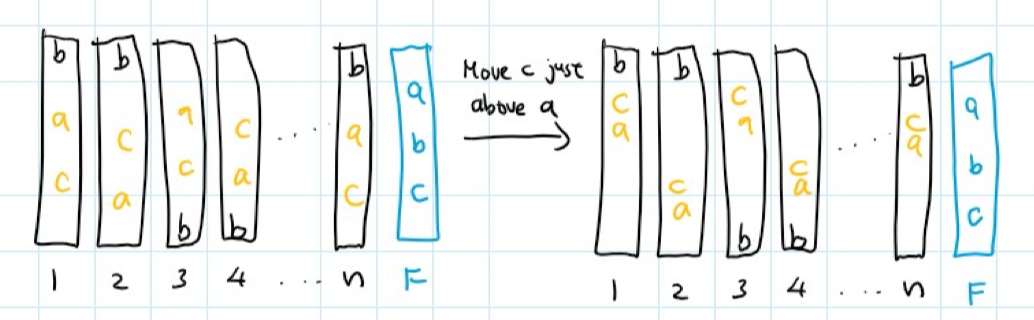
\includegraphics[width=\textwidth]{voting_1.png}
		      	\end{figure}
		      \end{center}
		\item Find a potential voter that can be a dictator. Take an arbitrary voter preference $P \in L^n$. Create a sequence of preferences $P_0, P_1, ..., P_n$ by first moving $b$ to the bottom, then move $b$ to the top one voter at a time. 
		      \newpage
		      \begin{center}
		      	\begin{figure}[h!]
		      		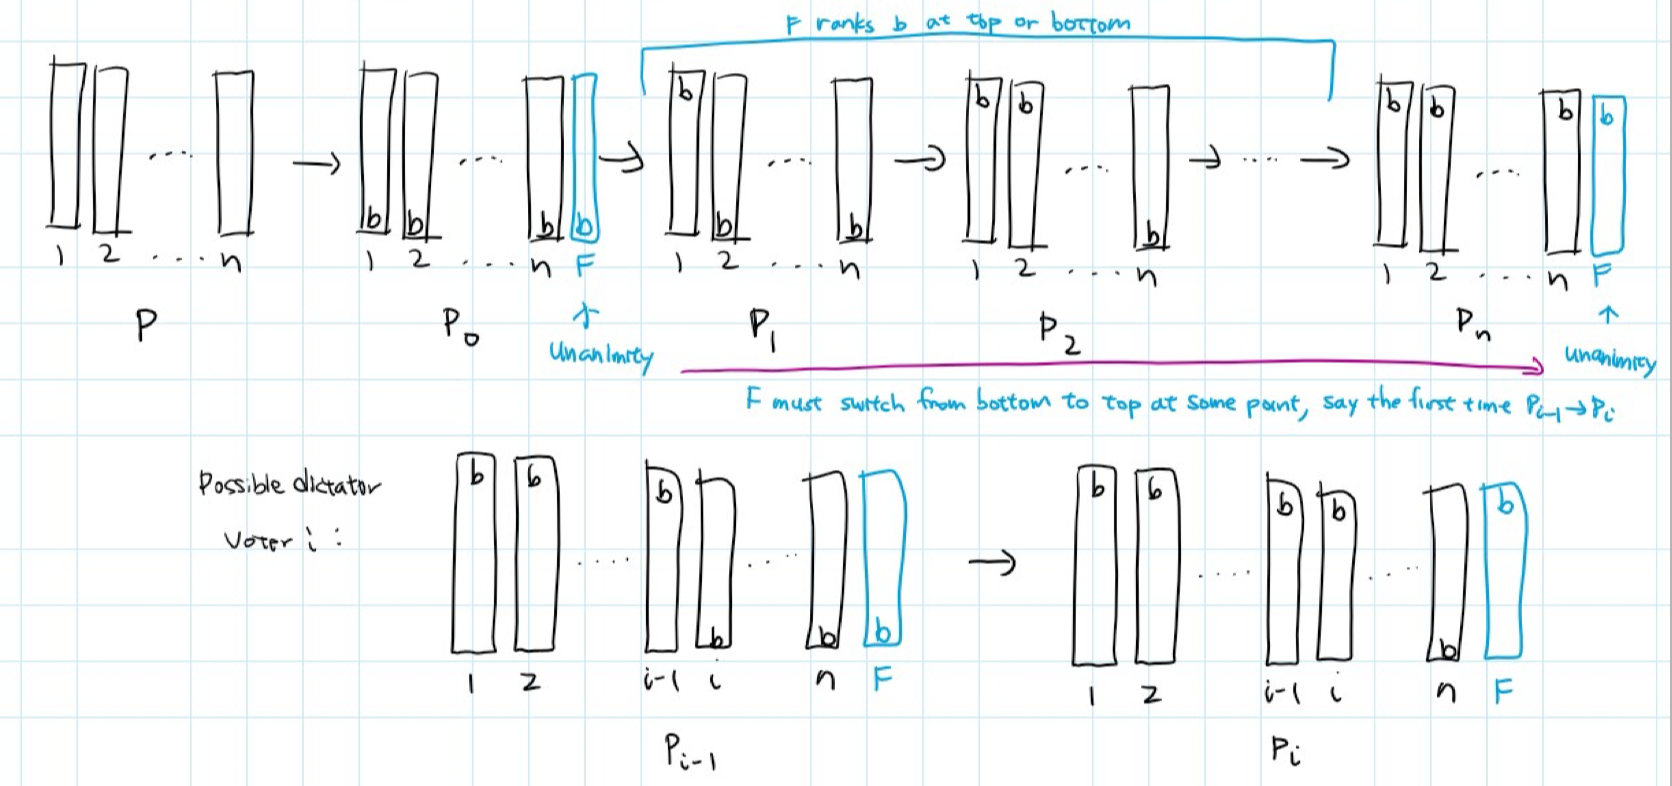
\includegraphics[width=\textwidth]{voting_2.png}
		      	\end{figure}
		      \end{center}
		\item Let $a, c$ be two candidates other than $b$. They exists since there are at least 3 canddiates. We will show that $F$ agrees with voter $i$ on the relative ranking $a, c$. Without loss of generality, voter $i$ ranks $a$ above $c$ in the original $P$. Create a new voter preference $p^*$ from $p_i$ by moving $a$ to the top of the list for voter $i$. 
		      
		      \begin{center}
		      	\begin{figure}[h!]
		      		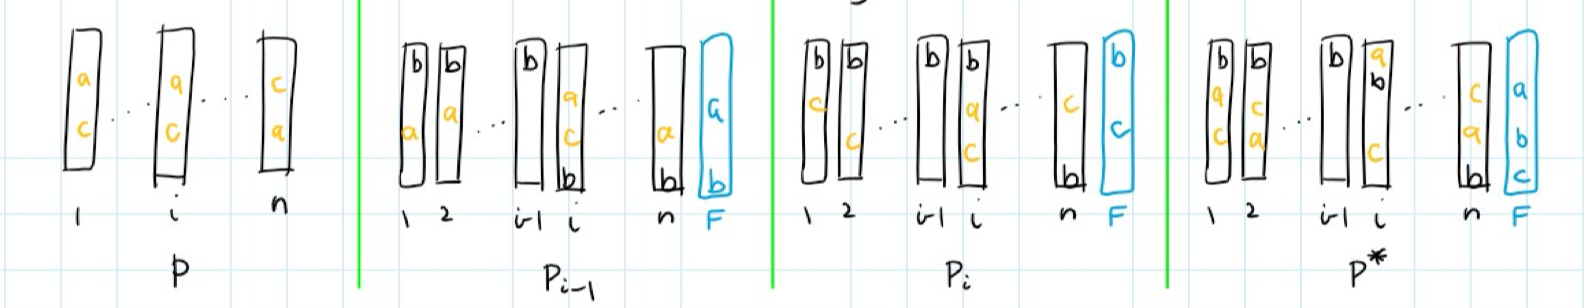
\includegraphics[width=\textwidth]{voting_3.png}
		      	\end{figure}
		      \end{center}
		      
		      Note that, between $P$ and $P^*$, the relative rankings of $a, c$ do not change. By IIA, $F$ ranks $a, c$ the same $P$ and $P^*$. 
		      
		      The goal is to show that $F$ ranks $a$ above $c$ in $P^*$ (agreeing with voter $i$). 
		      
		      Compare $P_{i-1}$ and $P^*$, the relative rankigns of $a, b$ do not change. By IIA, $F$ ranks $a, b$ the same in $P_{i-1}$ and $P^*$. 
		      
		      $F$ ranks $b$ at the bottom in $P_{i-1}$, so $a > b$ for both $P_{i-1}$ and $P^*$. 
		      
		      Compare $P_{i}$ and $P^*$, the relative rankigns of $b, c$ do not change. By IIA, $F$ ranks $b, c$ the same in $P_{i}$ and $P^*$. 
		      
		      $F$ ranks $b$ at the top in $P_{i}$, so $b > c$ for both $P_{i}$ and $P^*$. 
		      
		      By transitivity, $F$ ranks $a > c$, which matches the ramking for voter $i$. So $F$ agrees with voter $i$ on the relative rankings of any two candidates other than $b$. 
		      
		\item Let $d$ be any candidate other than $b$. We will show that $F$ agrees with voter $i$ on $b, d$. 
		      
		      There exists candidate $e$ that is not $b, d$ (since we have $\geq 3$ candidates). Run the arguments from 2 and 3 with $e$ instead of $b$ would gives us that a voter $j$ such that $F$ agrees with voter $j$ for any two candidates that are not $e$. We will show that $i = j$. 
		      
		      Suppose otherwise, say $j < i$. Consdier $P_{i-1}$. $F$ ranks $b$ at the bottom, so $d > b$. For voter $j$, $d$ is lower than $b$, and $F$ must agree with voter $j$ in all cases not involving $e$. So $F$ ranks $b > d$. This contradicts antisymmetric property of $F$. 
		      
		      \begin{center}
		      	\begin{figure}[h!]
		      		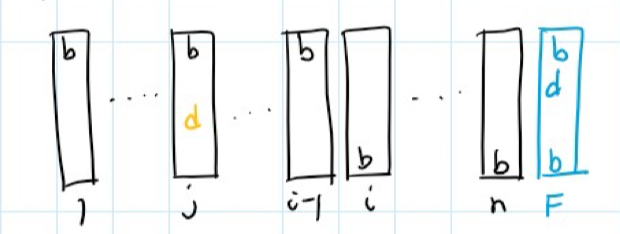
\includegraphics[width=.6\textwidth]{voting_4.png}
		      	\end{figure}
		      \end{center}
		      
		      Suppose $j > i$. Consdier $P_i$, $F$ ranks $b > d$. But voter $j$ ranks $d$ over $b$. And $F$ agrees with voter $j$. So $d > b$ in $F$. Contradiction. 
		      \begin{center}
		      	\begin{figure}[h!]
		      		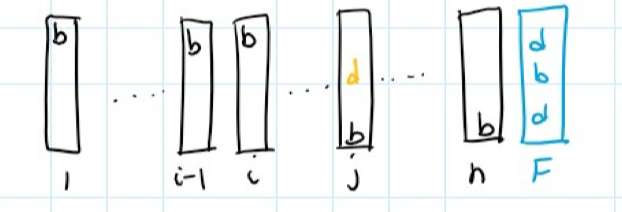
\includegraphics[width=.6\textwidth]{voting_5.png}
		      	\end{figure}
		      \end{center}
		      
		      So, $i = j$. 
	\end{enumerate}
	
	So, $F$ agrees with voter $i$ on the relative rankings of any two candidates. Hence voter $i$ is a dictator. 
	
	\section{Gibbarth-Satterthwaite Theorem}
	A social choice function $f: L^n \rightarrow A$ selects one candidate to represent the preferences of the voters. Just like social welfare functions, there cannot be a social choice function with good properties without the bad. 
	
	Good property: Strategy-proof
	
	\begin{definition}
		A voter cannot change the society's choice to something they like better by changing their preferences. 
			
		We say that $f$ can be \textbf{\underline{strategically manipulated}} by voter $i$ if there exists $a, b \in A$, $(<_1, ..., <_n) \in L^n$ and $<'_i \in L$ such that $a <_i b$ (voter $i$ prefers $b$ over $a$), $f(<_1, ..., <_n) = a$ (society picks $a$), and $f(<_1, ..., <'_i, ..., <_n) = b$ (society picks the one that voter $i$ likes better when they change their vote). We say $f$ is \textbf{\underline{strategy-proof}} if $f$ cannot be strategically manipulated. 
	\end{definition}
	
	Note: A strategy-proof voting mechanism will ensure that voters vote truthfully, so truthful voting is a dominant strategy. 
	
	Bad property: Dictatorship. There exists a voter $i$ such that $f$ will always choose the candidate at the top of voter $i$'s list. 
	
	\begin{theorem}
		\textbf{Gibbarth-Satterthwaite Theorem}: Any strategy-proof social choice function onto a set of at least 3 candidates is a dictatorship. 
	\end{theorem}
	
	The main ideas for the proof: Assume $f: L^n \rightarrow A$ is strategy-proof. Construct a social welfare function $F: L^n \rightarrow L$ as follows: 
	\begin{center}
		\begin{figure}[h!]
			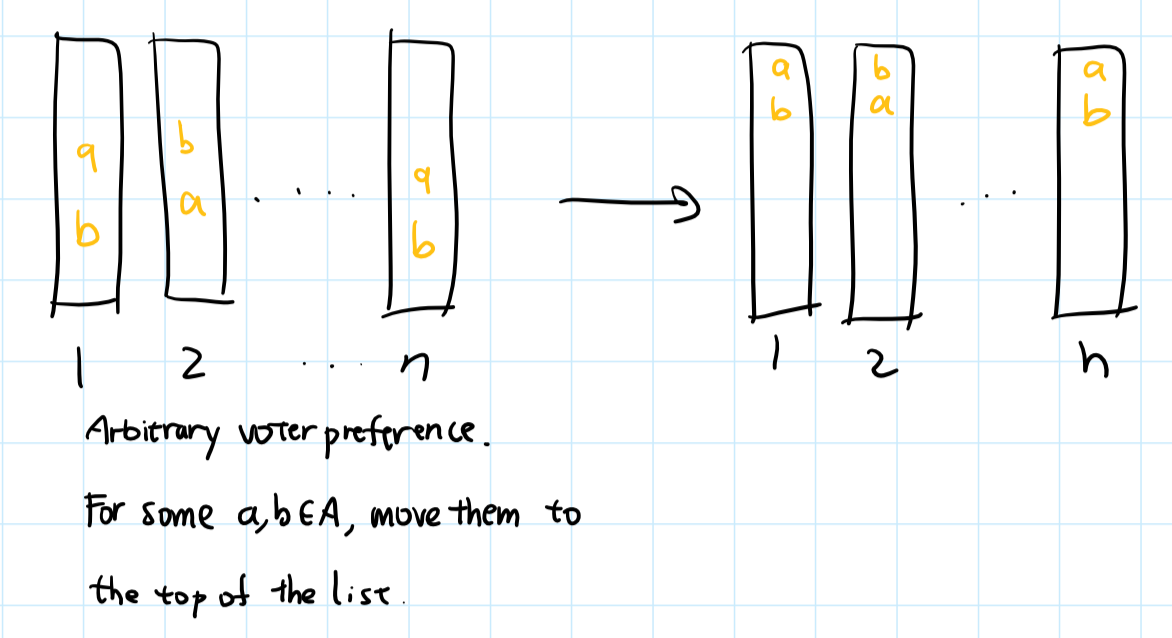
\includegraphics[width=\textwidth]{voting_6.png}
		\end{figure}
	\end{center}
	One can show that $f$ will pick either $a$ or $b$. If $f$ picks $a$, then set $a > b$ in $F$. Otherwise, set $b > a$. Do this for all pairs $a, b$. We have constructed $F$. 
	
	We need to show that $F$ is a total order, i.e. antisymmetric and transitive. 
	
	Then, $F$ satisfies unanimity and IIA. Since there are at least 3 candidates, Arrow's Impossibility theorem implies that $F$ is a dictatorship. The dictator for $F$ is also the dictator for $f$. 
	
	Up to now, the mechanism design for voting seems to be all bad news. Research has been done to find ``escape routes'' to find strategy-proof mechanisms without the bad consequences. For example, we may restrict voter preferences in some way, or introduce money into a voter's utility (similar to mechanism design for auctions). 
\end{document}